% Ovo je glavni fajl za generiranje predloska dokumenta doktorske disertacije Elektrotehnickog fakulteta u Sarajevu. 
% Verzija: 11. maj 2018. godine 

% Autor: Emir Sokic , esokic@etf.unsa.ba
% Bazirano na predlosku koji se koristi na FER Zagreb

%%%%%%%%%%%%%%%%%%%%%%%%%%%%%%%%%%%%%%%%%%%%%%%%%%%%%%%%%%%%%%%%%%%%%%
%%%%%%%%%%%%%%%%%%%%%%%%% POSTAVKE %%%%%%%%%%%%%%%%%%%%%%%%%%%%%%%%%%%
%%%%%%%%%%%%%%%%%%%%%%%%% NE MIJENJATI %%%%%%%%%%%%%%%%%%%%%%%%%%%%%%%
%%%%%%%%%%%%%%%%%%%%%%%%%%%%%%%%%%%%%%%%%%%%%%%%%%%%%%%%%%%%%%%%%%%%%%

\documentclass[12pt,oneside, a4paper]{book}

%Ovo su paketi koji se koriste za kompajliranje dokumenta
%Vecina paketa je ukljucena po defaultu u texlive 2013 i novijim verzijama
\usepackage{xcolor}
\usepackage{graphicx}
\usepackage{rotating}
\usepackage[T1]{fontenc}
\usepackage[utf8]{inputenc}
\usepackage{cmap}
% Napomena: LaTeX nema 'bosnian' opciju za babel; 'croatian' je najbliža
% dostupna lokalizacija koja korektno obrađuje bosanska dijakritička slova.
\usepackage[croatian]{babel}
\usepackage[unicode]{hyperref}
\usepackage{mathptmx}
\usepackage{amscd}
\usepackage{amssymb}
\usepackage{amsmath}
\usepackage{amsfonts}
\usepackage[left=2.5cm,right=2.5cm,top=2.5cm,bottom=2.5cm]{geometry}
\usepackage{setspace} 
\usepackage{hhline}
\usepackage{enumerate}
\usepackage{delarray}
\usepackage{array}  
\usepackage{tabularx} 
\usepackage{multirow}  
\usepackage[bf, font=small]{caption}
\usepackage[labelfont=small, font=small]{subcaption}
\usepackage{wasysym}
\usepackage{subeqnarray}
\usepackage{pdflscape} % setting page into landscape view
\usepackage{enumitem} % for itemize lists
\usepackage[toc,page]{appendix}
\newcommand{\HRule}{\rule{\linewidth}{0.5mm}}
\usepackage{makeidx}
\usepackage{nomencl}
\usepackage{listings}
\lstset{basicstyle=\ttfamily,breaklines=true}
\usepackage{courier}
% Podesavanje izgleda zaglavlja i podnozja strana
\usepackage{fancyhdr} 
\usepackage{booktabs}
\usepackage{float}
\usepackage{tikz}
\usetikzlibrary{shapes.geometric, arrows.meta, positioning, calc}

\fancypagestyle{plain}{%
  \fancyhf{}% Clear header/footer
  \fancyfoot[OR]{{\thepage}}%
  \fancyfoot[EL]{{\thepage}}%
  \renewcommand{\headrulewidth}{0pt}%
}



%Opcionalno
%\linespread{1.3}
%\setlist{nolistsep}   % setting for itemize lists
%\renewcommand{\thefootnote}{\fnsymbol{footnote}}  % to get unnumbered footnotes

% Adding a dot after chapter number in TOC 
%\let\savenumberline\numberline
%\def\numberline#1{\savenumberline{#1.}}

%\pagestyle{fancyplain}

%\rfoot{\thepage}
% iskljucivanje broja strane iz Sadrzaja, Popisa slika i Popisa tabela
\AtBeginDocument{\addtocontents{toc}{\protect\thispagestyle{empty}}}
\AtBeginDocument{\addtocontents{lof}{\protect\thispagestyle{empty}}}
\AtBeginDocument{\addtocontents{lot}{\protect\thispagestyle{empty}}}

%\rhead{\slshape \nouppercase \leftmark}
%\lhead{} %delete left header


%Podesavanje izgleda referenci
\usepackage[square, numbers, sort]{natbib} 

%Promjena naziva pojedinih poglavlja sa Hrvatskog na Bosanski
% Bibliography u "Literatura"
\addto\captionscroatian{%
  \renewcommand{\bibname}{Literatura}
  \renewcommand{\tablename}{Tabela}
  \renewcommand{\nomname}{Popis oznaka}
  \renewcommand{\indexname}{Indeks pojmova}
  \renewcommand{\lstlistingname}{Program}
}
%"Popis tablica" u "Popis tabela"
\addto\captionscroatian{\renewcommand{\listtablename}{Popis tabela}}
\addto\captionscroatian{\renewcommand\appendixname{Prilog}}
\addto\captionscroatian{\renewcommand\appendixpagename{Prilozi}}
\renewcommand\appendixtocname{Prilozi}

\makeindex
\makenomenclature

%\usepackage{etoolbox}
%\patchcmd{\chapter}{\thispagestyle{plain}}{\thispagestyle{fancyplain}}{}{}
\setlength{\parindent}{0pt}

\begin{document}

%%%%%%%%%%%%%%%%%%%%%%%%%%%%%%%%%%%%%%%%%%%%%%%%%%%%%%%%%%%%%%%%%%%%%%
%%%%%%%%%%%%%%%%%%%%%%%%% OSNOVNI DOKUMENT %%%%%%%%%%%%%%%%%%%%%%%%%%%
%%%%%%%%%%%%%%%%%%%%%%%%%%%%%%%%%%%%%%%%%%%%%%%%%%%%%%%%%%%%%%%%%%%%%%

\frontmatter

%%%%%%%%%%%%%%%%%%%% NASLOVNA STRANA %%%%%%%%%%%%%%%%%%%%%%%%
\begin{titlepage}
\begin{center}


\includegraphics[width=0.25\textwidth]{etf-logo.png}~\\[0.1cm]
\textsc{\Large Univerzitet u Sarajevu}\\[0.2cm]  
\textsc{\Large Elektrotehnički fakultet}\\[0.2cm] 
\textsc{\Large Odsjek za računarstvo i informatiku }\\[3cm]\HRule \\[0.5cm] 
{\huge \bfseries Eksperimentalna analiza timing side-channel napada na RSA} \\[0.4cm] 
\HRule \\[0.5cm]

\textsc{\Large Završni rad}\\[0.4cm]
\textsc{\Large - Prvi ciklus studija - }\\[1.5cm]

% Author and supervisor 
\textbf{ 
\Large Student:\\  
\Large Tarik Fetahović\\[1cm]  
\Large Mentor: \\[0.2cm] 
\Large Prof. dr Saša Mrdović.} 
\vfill

% Bottom of the page  
{\large Sarajevo, \\maj 2026.}

\end{center} 
\end{titlepage}

% Sažetak (na Bosanskom jeziku) i Abstract (na Engleskom jeziku),
% postavka rada i izjava o autentičnosti su dati kao odvojeni fajlovi

%%%%%%%%%%%%%% SAŽETAK I ABSTRACT %%%%%%%%%%%%%%%%%%%%%%%%%%%%%%%%
\pagebreak

\section*{Sažetak}

U radu se eksperimentalno analiziraju timing i cache side-channel napadi na RSA kriptosistem. Fokus je na statističkoj detekciji i iskorištavanju vremenskih razlika uzrokovanih uslovnim grananjem u square-and-multiply algoritmu, te na Flush+Reload napadu koji iskorištava dijeljeni LLC (\textit{Last Level Cache}). Provedeno je sedam eksperimenata na modernom procesoru (Intel i5-1335U): detekcija timing leaka, averaging napad, potpuna rekonstrukcija 64-bitnog privatnog ključa, sistematska multi-bit analiza, evaluacija utjecaja kompajlerskih optimizacija, analiza RSA blindinga kao kontramjere, te Flush+Reload cache napad.

Rezultati pokazuju da naivna implementacija ima mjerljiv timing leak od $\approx 76$ CPU ciklusa po bitu ($p < 10^{-50}$, Cohen-ov $d = 0{,}134$), koji omogućava potpunu slijepu rekonstrukciju ključa sa 100\% tačnošću uz 5000 mjerenja po bitu (teorijski dovoljno i $K \approx 2000$ za 100\% tačnost po bitu). Constant-time implementacija potpuno eliminiše leak ($p = 0{,}84$, $d \approx 0$). Kompajlerske optimizacije (O0--O3) ne eliminišu ranjivost, a RSA blinding ne štiti od branch-zavisnih leaka. Flush+Reload napad potvrđuje bimodalnu distribuciju reload latencija s razlikom od $\approx 342$ ciklusa između cache hit i cache miss, što omogućava klasifikaciju bita iz jednog mjerenja.

\bigskip
\textbf{Ključne riječi}: RSA, timing side-channel napad, Flush+Reload, square-and-multiply, constant-time, statistička analiza, rekonstrukcija ključa, RSA blinding

\section*{Abstract}

This thesis experimentally analyzes timing and cache side-channel attacks on the RSA cryptosystem, focusing on statistical detection and exploitation of timing differences caused by conditional branching in the square-and-multiply algorithm, as well as the Flush+Reload attack exploiting the shared Last Level Cache (LLC). Seven experiments were conducted on a modern processor (Intel i5-1335U): timing leak detection, averaging attack, full 64-bit private key reconstruction, systematic multi-bit analysis, compiler optimization impact evaluation, RSA blinding countermeasure analysis, and Flush+Reload cache attack.

Results demonstrate that the naive implementation exhibits a measurable timing leak of $\approx 76$ CPU cycles per bit ($p < 10^{-50}$, Cohen's $d = 0.134$), enabling complete blind key reconstruction with 100\% accuracy using 5000 measurements per bit (with $K \approx 2000$ theoretically sufficient for 100\% per-bit accuracy). The constant-time implementation fully eliminates the leak ($p = 0.84$, $d \approx 0$). Compiler optimizations (O0--O3) do not eliminate the vulnerability, and RSA blinding does not protect against branch-dependent leaks. The Flush+Reload attack confirms a bimodal reload latency distribution with $\approx 342$ cycle separation between cache hit and miss, enabling single-measurement bit classification.

\bigskip
\textbf{Keywords}: RSA, timing side-channel attack, Flush+Reload, square-and-multiply, constant-time, statistical analysis, key reconstruction, RSA blinding


%%%%%%%%%%%%%%%%%%%% POSTAVKA RADA %%%%%%%%%%%%%%%%%%%%%%%%%%%%%%%
%%%%%%%%%%%%%%%%%%%% POSTAVKA RADA %%%%%%%%%%%%%%%%%%%%%%%%%%%%%%%
\thispagestyle{plain}
\begin{flushleft}
\textbf{Elektrotehnički fakultet, Univerzitet u Sarajevu}\\
\textbf{Odsjek za računarstvo i informatiku}\\
\textbf{Prof. dr Saša Mrdović, dipl.el.ing}\\


\textbf{Sarajevo, april 2026(datum) }\\
\end{flushleft}

\begin{center}
\vspace{2cm}
{\Large Postavka zadatka završnog rada I ciklusa:}\\
\vspace{0.2cm}
{\large \textbf{Eksperimentalna analiza timing side-channel napada na RSA}}
\end{center}

\vspace{0.5cm}
U okviru rada je potrebno razviti \LaTeX\ predložak za izradu završnog rada prvog ciklusa studija. U radu je potrebno:
\begin{itemize}
\item objasniti opći postupak za izradu i pisanje završnih radova prvog ciklusa studija, poštivajući odgovarajuće Pravilnike,
\item dati kratko uputstvo za korištenje .tex dokumenata, pisanje slika, tabela i relacija, generisanje sadržaja, popisa slika i tabela i sl.
\item dati kratko upusto za generiranje odgovarajućih .pdf dokumenata iz odgovarajućih .tex fajlova,
\end{itemize}
Preporučuje se korištenje TexLive \LaTeX\ podrške, verzije 2013 ili novije.

\textbf{Napomena: U dijelu "Postavka" se stavlja postavka rada koju je specificirao mentor prilikom davanja teme. Naročito obratiti pažnju na naslov rada koji mora biti konzistentan tokom cijelog dokumenta, i usaglašen sa temom upisanom u informacioni sistem (npr. Zamger). Na ovoj stranici se potpisuje mentor prije nego se radovi odnesu u studentsku službu.}


\vspace{1cm}
\textbf{Polazna literatura:}

\begin{itemize}
\item[]  [1] Sonka, M., Hlavec, V., Boyle, R., "Image Processing, Analysis, and Machine Vision", Thomson, 2008.
\item[] [2] Lee, E.A., Varaiya, P., "Structure and Interpretation of Signals and Systems", Electrical Engineering \& Computer Science University of California, Berkeley, 2000

\end{itemize}


\begin{center}
\vspace{2cm}
\makebox[8cm]{\hrulefill} \\
Vanr. prof. dr Alessandro Volta, dipl. ing. el.\\
\end{center}







%%%%%%%%%%%%%%%%%%%% IZJAVA AUTORA %%%%%%%%%%%%%%%%%%%%
\include{izjava}

%%%%%%%%%%%%%%%%%%%%% SADRŽAJ %%%%%%%%%%%%%%%%%%%%%%%%%
%\clearpage
\tableofcontents

%%%%%%%%%%%%%%% POPIS SLIKA %%%%%%%%%%%%%%%%%%%%%%%%%%%
%\clearpage
\listoffigures
\addcontentsline{toc}{chapter}{Popis slika}

%%%%%%%%%%%%%%% POPIS TABELA %%%%%%%%%%%%%%%%%%%%%%%%%%
%\clearpage
\listoftables
\addcontentsline{toc}{chapter}{Popis tabela}

%%%%%%%%%%%%%%% POPIS KRATICA %%%%%%%%%%%%%%%%%%%%%%%%%
%\chapter*{Popis kratica}
\addcontentsline{toc}{chapter}{Popis kratica}
\label{ch:kratice}

\begin{description}[leftmargin=4.2cm, labelwidth=4cm, font=\normalfont\bfseries]
\item[AES]      \textit{Advanced Encryption Standard} -- napredni standard enkripcije
\item[CPU]      \textit{Central Processing Unit} -- centralna procesorska jedinica
\item[CDF]      \textit{Cumulative Distribution Function} -- kumulativna funkcija distribucije
\item[CRT]      \textit{Chinese Remainder Theorem} -- kineski teorem o ostacima
\item[DRAM]     \textit{Dynamic Random-Access Memory} -- dinamička memorija s nasumičnim pristupom
\item[DSS]      \textit{Digital Signature Standard} -- standard digitalnog potpisa
\item[DPA]      \textit{Differential Power Analysis} -- diferencijalna analiza snage
\item[E-core]   \textit{Efficiency Core} -- jezgro efikasnosti (Intel hibridna arhitektura)
\item[FIPS]     \textit{Federal Information Processing Standard} -- savezni standard za obradu informacija
\item[GCC]      \textit{GNU Compiler Collection} -- zbirka GNU kompajlera
\item[GCHQ]     \textit{Government Communications Headquarters} -- britanska obavještajna agencija
\item[HSM]      \textit{Hardware Security Module} -- hardverski sigurnosni modul
\item[HTTPS]    \textit{Hypertext Transfer Protocol Secure} -- sigurni HTTP protokol
\item[LLC]      \textit{Last Level Cache} -- keš memorija zadnjeg nivoa (tipično L3)
\item[LSB]      \textit{Least Significant Bit} -- najmanje značajan bit
\item[MSB]      \textit{Most Significant Bit} -- najznačajniji bit
\item[NIST]     \textit{National Institute of Standards and Technology} -- američki nacionalni institut za standarde
\item[P-core]   \textit{Performance Core} -- jezgro performansi (Intel hibridna arhitektura)
\item[PLT]      \textit{Procedure Linkage Table} -- tablica za dinamičko povezivanje procedura
\item[PRNG]     \textit{Pseudo-Random Number Generator} -- generator pseudo-slučajnih brojeva
\item[RDTSC]    \textit{Read Time-Stamp Counter} -- x86 instrukcija za čitanje TSC-a
\item[RDTSCP]   \textit{Read Time-Stamp Counter and Processor ID} -- serijalizovana varijanta RDTSC-a
\item[RSA]      \textit{Rivest-Shamir-Adleman} -- asimetrični kriptografski algoritam
\item[SNR]      \textit{Signal-to-Noise Ratio} -- omjer signala i šuma
\item[SPA]      \textit{Simple Power Analysis} -- jednostavna analiza snage
\item[SSH]      \textit{Secure Shell} -- protokol za sigurnu udaljenu vezu
\item[TLB]      \textit{Translation Lookaside Buffer} -- međuspremnik za prevođenje adresa
\item[TLS]      \textit{Transport Layer Security} -- protokol za sigurnost transportnog sloja
\item[TSC]      \textit{Time Stamp Counter} -- brojač vremenskih oznaka procesora
\end{description}


%%%%%%%%%%%%%%% POPIS OZNAKA %%%%%%%%%%%%%%%%%%%%%%%%%%%
\cleardoublepage % start new page
\pagestyle{fancyplain} % puts headers/footers back on
\fancyhf{}
\lhead{\nouppercase{\fancyplain{}{\leftmark}}}
\renewcommand{\chaptermark}[1]{\markboth{#1}{}}
\renewcommand{\footrulewidth}{0.4pt} %draw foot line
\lfoot{\slshape Fetahović, T., "Eksperimentalna analiza timing side-channel napada na RSA"}
\rfoot{\thepage}
\cfoot{}

%%%%%%%%%%%%%%%%%%%%%%%%%%%%%%%%%%%%%%%%%%%%%%%%%%%%%%%%%%%%%%%%%%%%
\mainmatter

%%%%%%%%%%%%%%%%%%%%%%%%%%%%%%%%%%%%%%%%%%%%%%%%%%%%%%%%%%%%%%%%%%%%
%%%%%%%%%%%%%%%%%%%%%%%%% POGLAVLJA %%%%%%%%%%%%%%%%%%%%%%%%%%%%%%%%
%%%%%%%%%%%%%%%%%%%%%%%%%%%%%%%%%%%%%%%%%%%%%%%%%%%%%%%%%%%%%%%%%%%%

%Poglavlja je najbolje raditi u odvojenim fajlovima
%Poglavlje 1
% poglavlje_1.tex — Uvod

\chapter{Uvod}
\label{ch:uvod}

\section{Obrazloženje teme}
\label{sec:obrazlozenje}

Sigurnosni protokoli poput HTTPS-a ili SSH-a u pozadini koriste asimetrične kriptografske algoritme da uspostave sigurnu vezu, a RSA je među njima jedan od najrasprostranjenijih. Sigurnost RSA-a se zasniva na težini faktorizacije proizvoda dva vrlo velika prosta broja \cite{rivest1978}.

Matematička robusnost kriptografskog algoritma ne implicira i sigurnost njegove konkretne implementacije. Softver može nenamjerno otkriti informacije o tajnom ključu kroz mjerljive fizičke popratne efekte kao što je vrijeme izvršavanja koda ili varijacije u naponu uređaja na kojem je pokrenut algoritam. Takvi napadi se klasifikuju kao napadi bočnim kanalima (\textit{side-channel attacks}), pri čemu se umjesto matematičkih slabosti napada fizički proces izvođenja operacija.

Standardna implementacija RSA modularne eksponencijacije zasniva se na algoritmu square-and-multiply. U njemu se za svaki bit privatnog eksponenta čija je vrijednost 1 izvodi dodatna operacija množenja koja nije prisutna kada je vrijednost bita 0. Budući da to jedno množenje unosi mjerljivo vremensko odstupanje od nekoliko desetina CPU ciklusa, napadač koji može mjeriti razlike u trajanju operacija dešifriranja dovoljan broj puta može statističkom metodom usrednjavanja, bit po bit, rekonstruisati tajni ključ. Ovo je Paul Kocher demonstrirao 1996. godine na stvarnim uređajima \cite{kocher1996}, a Jean-François Dhem i koautori su pokazali konkretnu praktičnu realizaciju napada \cite{dhem1998}. Nekoliko godina kasnije, Brumley i Boneh su pokazali da napad funkcioniše i kroz mrežu, na različitim platformama i implementacijama, ciljajući stvarni OpenSSL server \cite{brumley2003}.

RSA je odabran kao cilj analize jer je najrasprostranjeniji asimetrični algoritam u postojećim sistemima, a square-and-multiply algoritam pruža jasan i izolovan timing signal pogodan za eksperimentalnu demonstraciju.

Za razliku od Brumley i Boneh koji su analizirali mrežni OpenSSL server, ovaj rad demonstrira timing napad u lokalnom okruženju na modernom procesoru s modernijom arhitekturom i provodi potpunu rekonstrukciju 64-bitnog privatnog ključa isključivo iz timing mjerenja.

Suštinski istraživački problem ovog rada je detekcija slabog signala u okruženju sa visokim nivoom šuma. Vremenska razlika koju unosi jedna operacija množenja zanemarljiva je u poređenju sa sistemskim šumom koji proizvode moderni procesori i operativni sistemi. Međutim, primjenom statističkih metoda usrednjavanja šum konvergira prema nuli, što omogućuje ekstrakciju tajnog ključa iz dovoljno velike serije uzoraka. Kako se ističe u sveobuhvatnom pregledu mikroarhitekturalnih timing napada \cite{ge2018}, upravo ova mogućnost ekstrakcije ključa iz naivnih implementacija čini sigurnost RSA algoritma i danas aktuelnom temom u kontekstu side-channel napada.

Pored demonstracije ranjivosti, rad evaluira i kontramjere: constant-time implementaciju koja potpuno eliminiše leak, RSA blinding čija ograničenja demonstriraju razliku između branch-zavisnih i operand-zavisnih timing leaka, te utjecaj kompajlerskih optimizacija na sigurnost.

\subsection{Doprinos rada}

Konkretni doprinosi ovog rada su:
\begin{itemize}
  \item Statistička kvantifikacija timing leaka na modernom procesoru (Intel i5-1335U, Raptor Lake), uključujući šest komplementarnih statističkih testova, bootstrap intervale povjerenja i analizu statističke snage (\textit{power analysis}).
  \item Potpuna slijepa rekonstrukcija 64-bitnog privatnog RSA ključa isključivo iz timing mjerenja sa 100\% tačnošću, pri čemu napadački kod nikada nije imao direktan pristup vrijednosti tajnog ključa.
  \item Empirijska evaluacija tri kontramjere: constant-time implementacije, RSA blindinga i utjecaja kompajlerskih optimizacija.
  \item Demonstracija Flush+Reload cache napada kao kvalitativno drugačijeg mehanizma detekcije s višestruko jačim signalom.
\end{itemize}

\section{Struktura rada}
\label{sec:struktura}

Poglavlje \ref{ch:teorija} obrađuje teorijske osnove neophodne za razumijevanje eksperimenta: RSA kriptosistem, square-and-multiply algoritam, klasifikaciju timing napada u kontekstu relevantne literature, te statističke metode korištene u analizi (t-test, Mann-Whitney U, Cohen-ov d, bootstrap intervali povjerenja, power analiza).

Poglavlje \ref{ch:implementacija} dokumentuje eksperimentalnu metodologiju: obje varijante modularne eksponencijacije (\textit{naive} i \textit{constant-time}), mehanizam preciznog mjerenja CPU ciklusa pomoću \texttt{RDTSCP} instrukcije, te dizajn eksperimenta zasnovan na uparenom pristupu (\textit{paired approach}).

Poglavlje \ref{ch:rezultati} predstavlja rezultate sedam provedenih eksperimenata: detekcija timing leaka, averaging napad, rekonstrukcija 64-bitnog ključa, sistematska multi-bit analiza, utjecaj kompajlerskih optimizacija, evaluacija RSA blindinga kao kontramjere, te Flush+Reload cache napad. Poglavlje se završava diskusijom o značaju rezultata.

Poglavlje \ref{ch:zakljucak} sumira ključna postignuća, formuliše preporuke za sigurniju implementaciju i navodi ograničenja istraživanja te moguće pravce daljeg rada.

U Prilogu \ref{app:hw_config} dokumentovana je konfiguracija eksperimentalnog okruženja i prikazani su ključni assembly isječci koji verificiraju ispravnost obje implementacije na razini mašinskog koda.


%Poglavlje 2
% poglavlje_2.tex — Teorijske osnove

\chapter{Teorijske osnove}
\label{ch:teorija}

\section{RSA kriptosistem}

RSA kriptosistem, koji su 1978. godine predložili Rivest, Shamir i Adleman \cite{rivest1978}, je prvi javno objavljeni praktično primjenjeni sistem enkripcije s javnim ključem.\footnote{Diffie i Hellman su 1976. predložili teorijski okvir za razmjenu ključeva javnim kanalom, ali nisu specificirali konkretan sistem enkripcije. Clifford Cocks iz britanskog GCHQ-a razvio je ekvivalent RSA-a 1973, ali je to ostalo klasificirano do 1997. \cite{cocks1973}} Temelji se na asimetričnom paru ključeva: javnom ključu koji se slobodno distribuira i privatnom ključu koji ostaje tajan.

\subsection{Generisanje ključeva}

Generisanje RSA ključeva odvija se u sljedećim koracima:

\begin{enumerate}
\item Odaberu se dva velika prosta broja $p$ i $q$, pri čemu je $p \neq q$.
\item Računa se \textit{modulus} $n = p \cdot q$.
\item Računa se Eulerova phi-funkcija (funkcija totijenta): $\varphi(n) = (p-1)(q-1)$.
\item Bira se javni eksponent $e$ takav da je $1 < e < \varphi(n)$ i $\gcd(e, \varphi(n)) = 1$.
\item Privatni eksponent $d$ je modularni inverz od $e$ po modulu $\varphi(n)$:
\begin{equation}
d \cdot e \equiv 1 \pmod{\varphi(n)}
\label{eq:privatekey}
\end{equation}
\end{enumerate}

Javni ključ je par $(e, n)$, a privatni ključ je $d$ (zajedno s $n$).

\subsection{Šifriranje i dešifriranje}

Za poruku $M$ ($0 \leq M < n$), šifriranje se vrši eksponenciranjem s javnim ključem:
\begin{equation}
C = M^e \bmod n
\label{eq:encrypt}
\end{equation}

Dešifriranje se vrši eksponenciranjem šifrirane poruke $C$ s privatnim ključem:
\begin{equation}
M = C^d \bmod n
\label{eq:decrypt}
\end{equation}

Ispravnost dešifriranja garantuje Eulerova teorema: $M^{e \cdot d} \equiv M^{k\varphi(n)+1} \equiv M \pmod{n}$ \cite{rivest1978}.

\subsection{Sigurnost RSA-a}

Sigurnost RSA-a se zasniva na pretpostavci da je faktorizacija produkta dva velika prosta broja $n = p \cdot q$ praktično neizvodljiva. Poznati najbrži algoritam faktorizacije za klasične računare (General Number Field Sieve) ima subeksponencijalnu složenost $O(\exp(c(\ln n)^{1/3}(\ln \ln n)^{2/3}))$ \cite{lenstra1993}. Za modulus od 2048 bita koji se danas preporučuje, ovo je računski nedostižno s poznatim klasičnim računarskim resursima.\footnote{Shorov kvantni algoritam može faktorizovati RSA modulus u polinomijalnom vremenu \cite{shor1994}, što je pokrenulo razvoj post-kvantnih kriptografskih standarda. NIST je 2024. finalizirao prve post-kvantne standarde (FIPS 203, 204, 205) \cite{nist_pqc2024}. Analiza u ovom radu ograničena je na klasično okruženje.}

Međutim, sigurnost algoritma ne implicira automatski sigurnost implementacije, i upravo tu nastaju side-channel ranjivosti koje su tema ovog rada.

\section{Modularna eksponencijacija}

Glavna operacija u RSA kriptosistemu je \textit{modularna eksponencijacija}: izračunavanje $M^d \bmod n$ za veliko $d$. Direktno uzastopno množenje $M$ sa samim sobom $d$ puta je računski neprihvatljivo: za $d \approx 2^{2048}$, to bi zahtijevalo $2^{2048}$ množenja. Umjesto toga, koristi se algoritam kvadriraj-i-množi, koji svodi kompleksnost na $O(\log_2 d)$ množenja.

\subsection{Kvadriraj-i-množi algoritam}

Neka su $d_{k-1}, d_{k-2}, \ldots, d_1, d_0$ biti privatnog eksponenta $d$ od MSB (najznačajnijeg) ka LSB (najmanje značajnom). Algoritam od lijeva do desno kvadriraj-i-množi \cite{menezes1996} je sljedeći:

\begin{lstlisting}[language=C, caption={Kvadriraj-i-množi algoritam (pseudokod)}, label=lst:sqm]
result = 1
za i od k-1 do 0:
    result = result * result mod n 
    ako je d[i] == 1:
        result = result * M mod n   
vrati result
\end{lstlisting}

\noindent Algoritam radi $k$ kvadriranja i tačno $w$ množenja, gdje je $w$ Hammingova težina eksponenta $d$ (broj jediničnih bita). Za nasumičan 2048-bitni eksponent (koji je preporučen za korištenje u produkcijskim sistemima), očekivana vrijednost $w$ je 1024, pa algoritam tipično izvodi oko 3072 modularne multiplikacije. Dijagram toka algoritma prikazan je na slici \ref{fig:sqm_flow}.

\begin{figure}[H]
\centering
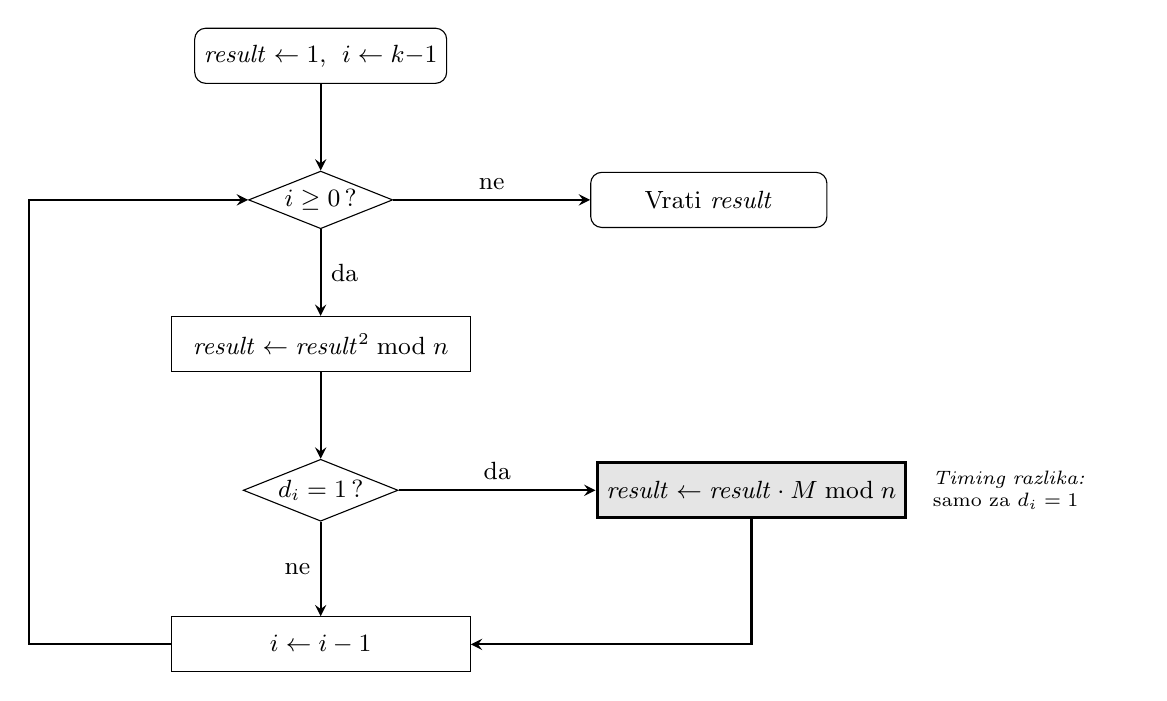
\begin{tikzpicture}[
    node distance=1.1cm,
    startstop/.style={rectangle, rounded corners, draw, minimum width=3cm, minimum height=0.7cm, text centered, font=\small},
    process/.style={rectangle, draw, minimum width=3.8cm, minimum height=0.7cm, text centered, font=\small},
    decision/.style={diamond, draw, aspect=2.5, text centered, font=\small, inner sep=1pt},
    leak/.style={rectangle, draw, minimum width=3.8cm, minimum height=0.7cm, text centered, font=\small, fill=gray!20, line width=1.2pt},
    arr/.style={->, >=stealth, thick}
]

\node[startstop] (init) {$\mathit{result} \leftarrow 1$,\; $i \leftarrow k{-}1$};
\node[decision, below=of init] (loop) {$i \geq 0$\,?};
\node[process, below=of loop] (sq) {$\mathit{result} \leftarrow \mathit{result}^2 \bmod n$};
\node[decision, below=of sq] (bit) {$d_i = 1$\,?};
\node[leak, right=2.5cm of bit] (mul) {$\mathit{result} \leftarrow \mathit{result} \cdot M \bmod n$};
\node[process, below=1.2cm of bit] (dec) {$i \leftarrow i - 1$};
\node[startstop, right=2.5cm of loop] (end) {Vrati $\mathit{result}$};

\draw[arr] (init) -- (loop);
\draw[arr] (loop) -- node[right, font=\small] {da} (sq);
\draw[arr] (loop) -- node[above, font=\small] {ne} (end);
\draw[arr] (sq) -- (bit);
\draw[arr] (bit) -- node[above, font=\small] {da} (mul);
\draw[arr] (bit) -- node[left, font=\small] {ne} (dec);
\draw[arr] (mul) |- (dec);
\draw[arr] (dec.west) -- ++(-1.8,0) |- (loop.west);

\node[right=0.2cm of mul, font=\scriptsize, text width=2.5cm, align=left] {\textit{Timing razlika:}\\samo za $d_i = 1$};

\end{tikzpicture}
\caption{Dijagram toka kvadriraj-i-množi algoritma. .}
\label{fig:sqm_flow}
\end{figure}

\subsubsection{Primjer}

Za $d = 11$ (binarno: $1011$) i $M = 5$, $n = 17$, tok algoritma je:

\begin{center}
\begin{tabular}{cccl}
\toprule
Bit $d[i]$ & Kvadriranje & Množenje & Međurezultat \\
\midrule
1 & $1^2 = 1$ & $1 \cdot 5 = 5$ & $5$ \\
0 & $5^2 = 25 \equiv 8$ & / & $8$ \\
1 & $8^2 = 64 \equiv 13$ & $13 \cdot 5 = 65 \equiv 14$ & $14$ \\
1 & $14^2 = 196 \equiv 9$ & $9 \cdot 5 = 45 \equiv 11$ & $11$ \\
\bottomrule
\end{tabular}
\end{center}

\noindent Rezultat: $5^{11} \bmod 17 = 11$, što se može verifikovati računski.

\subsection{Vremenska ranjivost algoritma}

Ključno zapažanje, ilustrirano dijagramom toka na slici \ref{fig:sqm_flow}, je da algoritam iz isječka koda \ref{lst:sqm} \textbf{ne izvodi isti broj operacija za sve vrijednosti bita eksponenta}:

\begin{itemize}
\item Za $d[i] = 0$: izvodi se \textbf{samo kvadriranje} (jedna modularna multiplikacija)
\item Za $d[i] = 1$: izvodi se \textbf{kvadriranje i množenje} (dvije modularne multiplikacije)
\end{itemize}

Svaka dodatna modularna multiplikacija dodaje mjerljiv prosječan trošak u CPU ciklusima. Razlika u trajanju po bitu jednaka je prosječnom trajanju jedne \texttt{mulmod} operacije, i to je izvor timing side-channel ranjivosti koju analiziramo u ovom radu.

\section{Side-channel napadi}

\subsection{Definicija i klasifikacija}

Side-channel napad iskorištava informacije koje "cure" iz fizičke realizacije kriptografskog sistema, a ne iz matematičke slabosti algoritma \cite{mangard2007}. Za razliku od kriptoanalize koja napada matematičku strukturu, side-channel napadi mjere fizički mjerljive veličine koje povezuju sa tajnim podacima. Glavne kategorije side-channel napada su:
\\

\textbf{Timing napadi.}
Mjeri se trajanje kriptografskih operacija. Signal može biti apsolutno trajanje, relativna razlika između operacija ili statistička distribucija trajanja \cite{kocher1996}.
\\

\textbf{Analiza potrošnje energije (\textit{power analysis}).}
Analizira se potrošnja uređaja na kojem se izvršava kriptografski sistem. Simple power analysis (SPA) vizualno analizira pojedinačne tragove strujne potrošnje, a differential power analysis (DPA) koristi statističku analizu većeg broja tragova s različitim ulaznim podacima \cite{kocher1999}.
\\

\textbf{Elektromagnetski napadi.}
Mjeri se elektromagnetna emisija uređaja tokom kriptografske operacije i izvodi se analiza signala. Primjenjivi su i bez fizičkog kontakta s uređajem \cite{gandolfi2001}.
\\

\textbf{Cache napadi.}
Iskorištavaju zajednički Last Level Cache (LLC) na višejezgrenim procesorima, gdje napadač može mjeriti vrijeme pristupa cache memoriji nakon njenog brisanja \cite{yarom2014}. Detaljno su opisani u sekciji \ref{sec:cache_attacks}.
\\

\textbf{Akustični napadi.}
Vrši se analiza zvukova koje emituju komponente računara tokom rada \cite{genkin2014}.

\subsection{Kocher-ov timing napad (1996)}
\label{sec:kocher}

Paul Kocher je 1996. godine demonstrirao da naivne implementacije Diffie-Hellman, RSA, DSS i sličnih protokola otkrivaju informaciju o privatnom ključu kroz trajanje operacije \cite{kocher1996}.

Osnovna ideja napada je sljedeća: napadač bira skup mjerenih poruka i za svaku bilježi trajanje kriptografske operacije. Mjerenja se grupišu prema hipotezi o vrijednosti pojedinog bita ključa. Ako je hipoteza ispravna, grupe mjerenja imat će statistički različite distribucije, jer je tajni bit konzistentno utjecao na trajanje. Ako je hipoteza pogrešna, distribucije će biti identične (šum).

Napad zahtijeva da napadač može:
\begin{enumerate}
\item Slati proizvoljne poruke na kriptografsku funkciju, i
\item Mjeriti trajanje operacije s dovoljnom preciznošću.
\end{enumerate}

\noindent U originalnom radu, Kocher je ciljao smart kartice koje nisu imale nikakvu zaštitu od timing napada. Pokazao je da je moguće rekonstruisati privatni ključ uz nekoliko stotina do nekoliko hiljada mjerenja.

\subsection{Brumley-Boneh mrežni napad (2003)}

Brumley i Boneh su 2003. godine proširili Kocher-ov napad na mrežni scenarij \cite{brumley2003}. Napadali su stvarni OpenSSL server na lokalnoj mreži, uzimajući u obzir mrežnu latenciju kao dodatni izvor šuma. Korištenjem tehnika kao što su:
\begin{itemize}
\item Slanje velikog broja zahtjeva za svaki bit,
\item Pažljiv odabir poruka koji pojačava timing razliku, i
\item Statistička analiza razlika u latenciji
\end{itemize}
\noindent uspjeli su rekonstruisati faktor RSA privatnog ključa. Ovaj napad je imao direktan praktičan utjecaj: OpenSSL je u verziji 0.9.7 implementirao RSA blinding kao kontramjeru.

\subsection{Cache timing side-channel napadi}
\label{sec:cache_attacks}

Za razliku od timing napada koji mjere ukupno trajanje operacije, cache timing side-channel napadi prate fizički pristup specifičnim memorijskim adresama kroz zajednički CPU cache. Na modernim višejezgrenim procesorima sva jezgra dijele LLC (Last Level Cache, tipično L3) i ovo dijeljenje, kombinovano s činjenicom da procesi koji koriste istu dijeljenu biblioteku (\texttt{.so} fajl) dijele i fizičke memorijske stranice te biblioteke, stvara tajni kanal između napadača i žrtve.

\subsubsection{Flush+Reload}

Flush+Reload napad \cite{yarom2014} odvija se u tri koraka koji se ponavljaju:

\begin{enumerate}
\item \textbf{Flush:} Napadač uklanja specifičnu cache liniju koristeći \texttt{clflush} instrukciju. Ova instrukcija je dostupna korisniku bez privilegija i garantovano uklanja adresu iz svih nivoa cache-a.
\item \textbf{Čekanje:} Napadač čeka dovoljno dugo da žrtva izvrši ciljanu operaciju.
\item \textbf{Reload:} Napadač mjeri kašnjenje ponovnog učitavanja (reload) te cache linije. Kratka latencija ($\approx$ L1/L2/LLC latencija, npr. 100 do 400 ciklusa) znači da je žrtva pristupila adresi, odnosno \textit{cache hit}, a duga latencija ($\approx$ DRAM latencija, npr. 500 do 1000 ciklusa) znači da žrtva nije pristupila adresi, odnosno \textit{cache miss}.
\end{enumerate}

\noindent Slika \ref{fig:flush_reload_phases} ilustrira ove tri faze i dva moguća ishoda.

\begin{figure}[H]
\centering
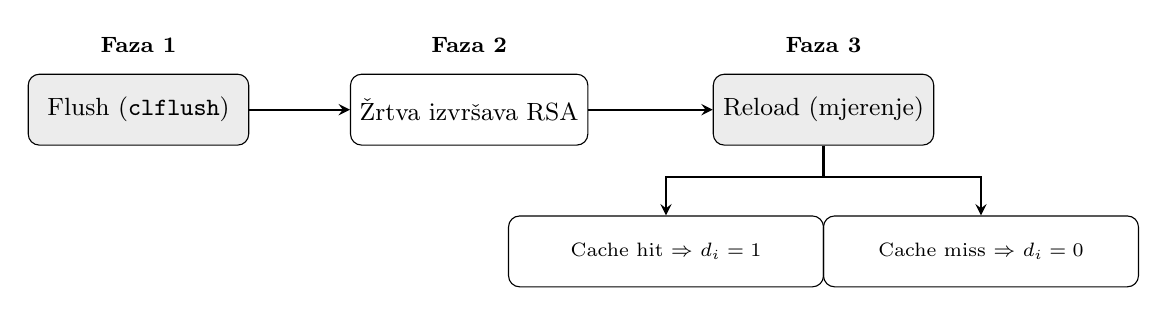
\begin{tikzpicture}[>=stealth,
    box/.style={rectangle, draw, rounded corners, minimum height=0.9cm, text centered, font=\small}]

\node[box, fill=gray!15, minimum width=2.8cm] (flush) at (0,0) {Flush (\texttt{clflush})};
\node[box, minimum width=3cm] (wait) at (4.2,0) {Žrtva izvršava RSA};
\node[box, fill=gray!15, minimum width=2.8cm] (reload) at (8.7,0) {Reload (mjerenje)};

\node[font=\footnotesize\bfseries, above=0.15cm of flush] {Faza 1};
\node[font=\footnotesize\bfseries, above=0.15cm of wait] {Faza 2};
\node[font=\footnotesize\bfseries, above=0.15cm of reload] {Faza 3};

\draw[->, thick] (flush) -- (wait);
\draw[->, thick] (wait) -- (reload);

\node[box, minimum width=4cm, font=\scriptsize] (hit) at (6.7,-1.8) {Cache hit  $\Rightarrow$ $d_i = 1$};
\node[box, minimum width=4cm, font=\scriptsize] (miss) at (10.7,-1.8) {Cache miss  $\Rightarrow$ $d_i = 0$};

\draw[->, thick] (reload.south) -- ++(0,-0.4) -| (hit.north);
\draw[->, thick] (reload.south) -- ++(0,-0.4) -| (miss.north);

\end{tikzpicture}
\caption{Faze Flush+Reload napada}
\label{fig:flush_reload_phases}
\end{figure}

Ključni preduvjet je \textbf{dijeljena memorija}: i napadač i žrtva moraju imati mapiranu istu fizičku stranicu. Ovo je automatski zadovoljeno za dijeljene biblioteke (npr.\ \texttt{libc.so}) gdje operativni sistem mapira jednu kopiju koda u fizičku memoriju, a oba procesa vide iste fizičke cache linije.

U kontekstu RSA napada, napadač cilja funkciju uslovnog množenja koja se poziva \textit{samo} kada je bit eksponenta jednak 1. Kada žrtva izvrši dekriptovanje pri čemu je ciljani bit eksponenta jednak 1, CPU učitava cache liniju te funkcije i napadač detektuje cache hit. Kada je bit jednak 0, funkcija se ne poziva i napadač detektuje cache miss.

\subsubsection{Prime+Probe}

Prime+Probe napad ne zahtijeva dijeljenu memoriju između napadača i žrtve, što ga čini primjenjivim čak i između virtualnih mašina. Napadač \textit{puni} (Prime) skup cache linija (cache set) vlastitim podacima, čeka da žrtva izvrši operaciju, a potom mjeri kašnjenje ponovnog pristupa (Probe) tim linijama. Ako je žrtva pristupila adresama koje mapiraju u iste cache linije, napadačeve linije su istisnute, što rezultira sporijim pristupom. Ovaj napad je složeniji za implementaciju i daje slabiji signal od Flush+Reload, ali funkcioniše i u scenarijima bez dijeljene memorije.

\subsection{Kontramjera: Constant-time implementacija}
\label{sec:ct_theory}

Constant-time implementacija je tehnika koja garantuje da trajanje kriptografske operacije ne zavisi od tajnih podataka. Princip je eliminacija uslovnog grananja (\textit{branchless programming}, programiranje bez grananja): umjesto \texttt{if-else} konstrukcije koja izvršava različit broj operacija za različite vrijednosti bita, uvijek se izvršavaju obje operacije (i kvadriranje i množenje), a rezultat se bira pomoću \textit{conditional move} (\texttt{cmov}) instrukcije ili aritmetičkog maskiranja, bez ikakvog skoka u kontrolnom toku. Na taj način, CPU izvršava identičan broj operacija i pristupa istim memorijskim adresama bez obzira na vrijednost bita, čime se eliminira i timing i cache side-channel. Konkretna implementacija opisana je u sekciji \ref{sec:ct_impl}.

\subsection{Kontramjera: RSA blinding}
\label{sec:blinding_theory}

RSA blinding je kontramjera uvedena u OpenSSL nakon Brumley-Boneh napada \cite{brumley2003}.  Zove se blinding ili zasljepljivanje jer "krije" podatke koji se obrađuju od vanjskih posmatrača. Princip je nasumičan odabir ulaza u eksponencijaciji:

\begin{enumerate}
\item Odabere se nasumičan $r$ takav da $\gcd(r, n) = 1$.
\item Izračuna se blinded ulaz: $M' = M \cdot r^e \bmod n$.
\item Eksponencijacija: $S' = (M')^d \bmod n$.
\item Unblinding: $S = S' \cdot r^{-1} \bmod n = M^d \bmod n$.
\end{enumerate}

Budući da napadač ne poznaje $r$, ne može povezati svoje poznate ulaze s internim međuvrijednostima. U realnom RSA s višepreciznom aritmetikom, ovo maskira operand-zavisne vremenske varijacije. Međutim, blinding ne mijenja eksponent $d$ i kontrolni tok ostaje identičan, što ima implikacije za branch-zavisna vremenska curenja analizirana u poglavlju \ref{ch:rezultati}.

\subsection{Model u ovom radu}

U ovom radu analiziran je lokalni timing napad s precizno definisanim modelom:
\\

\textbf{Napadač.}
Lokalni korisnik na istoj mašini, bez privilegija superkorisnika.
\\

\textbf{Mogućnosti napada.}
Pokretanje vlastitog koda i mjerenje trajanja kriptografskih operacija u CPU ciklusima. U ovom radu koriste se dva različita modela napadača, ovisno o eksperimentu:

\begin{itemize}
\item \textbf{Eksperimenti 1, 2, 4, 5 i 6 (karakterizacija signala):} Napadač može pozvati modularnu eksponencijaciju s proizvoljno odabranim eksponentima, uključujući parove koji se razlikuju samo u jednom bitu. Tajni ključ $S$ nije relevantan za ove eksperimente jer se napad bavi mjerenjem timing razlike između eksponenata koje napadač sam konstruiše.
\item \textbf{Eksperiment 3 (slijepa rekonstrukcija):} Napadač ne poznaje vrijednost tajnog ključa $S$ i nikada je ne vidi. Jedino što mu je dostupno jesu izmjerena trajanja: koliko dugo traje eksponencijacija s tajnim ključem za odabranu bazu $M$, te koliko bi trajala da je samo $i$-ti bit tog ključa bio obrnut i tu izmjenu sistem primjenjuje interno, na skrivenom $S$. Iz razlike tih trajanja napadač zaključuje koja je bila izvorna vrijednost bita i tako rekonstruiše ključ bit po bit \cite{kocher1996}.
\end{itemize}

\textbf{Ograničenja napada.}
Nema pristupa memoriji procesa žrtve; nema mrežnog pristupa; nema fizičkog pristupa hardveru.
\\

\textbf{Tajna.}
Privatni eksponent $d$ (64-bitni u ovom eksperimentu).
\\

\textbf{Javno poznato.}
Baza $M$, modulus $n$, broj bita eksponenta.
\\

Model prijetnji za Eksperiment 3 odgovara Kocher-ovom originalnom scenariju \cite{kocher1996}: napadač ne zna $S$ i rekonstruiše ga isključivo iz izmjerenih trajanja. Ovaj eksperiment demonstrira mehanizam curenja informacija pod idealiziranim lokalnim uslovima. Dok u realnom scenariju napadač bi imao ograničeniji pristup, npr.\ samo mrežni timing kao kod Brumley i Boneh \cite{brumley2003}, što bi zahtijevalo više mjerenja, ali bi temeljni mehanizam ostao isti.

Ovakav pristup je praktično primjenjiv svuda gdje postoji API za dekriptovanje: na smart karticama i HSM (\textit{Hardware Security Module}) uređajima, u dijeljenim kriptografskim servisima, te u TLS\,1.2 i starijim handshake protokolima s RSA ključnom razmjenom. U svim tim slučajevima napadač može slati pažljivo odabrane ulaze i mjeriti koliko traje svaki odgovor, bez ikakvog direktnog uvida u privatni ključ.

\section{Statističke metode u analizi side-channel napada}
\label{sec:statistika}

\subsection{Problem signala i šuma}

Trajanje kriptografskih operacija na modernom CPU-u nije konstantno. Brojni faktori doprinose varijabilnosti:

\begin{itemize}
\item \textbf{Promašaji cache-a}: Pristup memoriji koja nije u L1/L2/L3 cache-u dodaje stotine ciklusa latencije.
\item \textbf{Predikcija grananja}: Procesor predviđa smjer skokova; pogrešna predikcija dodaje kaznu od 10 do 20 ciklusa.
\item \textbf{OS preempcija}: Operativni sistem može prekinuti izvršavanje procesa u bilo kom trenutku (context switch).
\item \textbf{TLB i memorijske barijere}: Invalidacija prijevodnog međuspremnika (TLB) i memorijske barijere dodaju varijabilno kašnjenje.
\item \textbf{Toplotno ograničavanje}: Pregrijani procesor smanjuje frekvenciju, povećavajući trajanje.
\end{itemize}

\noindent Ukupni šum $\sigma$ u distribuciji trajanja obično je daleko veći od signala $\mu_1 - \mu_0$ koji odgovara jednoj \texttt{mulmod} operaciji. Omjer signal-šum (SNR) po jednom mjerenju definisan je kao:
\begin{equation}
\text{SNR} = \frac{|\mu_1 - \mu_0|}{\sigma_{\text{pool}}}
\label{eq:snr}
\end{equation}

\noindent gdje su $\mu_1$ i $\mu_0$ srednje vrijednosti trajanja za $\text{bit}=1$ i $\text{bit}=0$, a $\sigma_{\text{pool}}$ je ujedinjena standardna devijacija. SNR je ključna metrika jer određuje \textbf{izvodljivost napada}: ako je SNR visok, jedno mjerenje je dovoljno za detekciju bita; ako je nizak, napadač mora prikupiti mnogo mjerenja i usrednjiti ih. Ova veličina je po formi identična apsolutnoj vrijednosti Cohen-ovog $d$ (jednačina \ref{eq:cohens_d}): SNR $= |d|$. Obje metrike se koriste jer $d$ ima standardiziranu interpretaciju veličine efekta (mali/srednji/veliki), dok SNR direktno određuje minimalan broj mjerenja $K_{\min}$ potrebnih za uspješan napad. U ovom eksperimentu SNR $= |d| \approx 0{,}134$, što znači da je signal oko 7,5 puta manji od šuma i da je pojedinačno mjerenje nepouzdano.

\subsection{Usrednjavanje i centralna granična teorema}

Temeljni princip koji omogućava timing napad uprkos niskom SNR-u po jednom mjerenju je \textit{usrednjavanje} (averaging). Centralna granična teorema garantuje da srednja vrijednost $K$ nezavisnih mjerenja konvergira ka pravoj sredini bez obzira na oblik distribucije, što je od ključne važnosti jer distribucije CPU trajanja nisu normalne. Ako napadač prikupi $K$ nezavisnih mjerenja za isti bit i usrednji ih, standardna devijacija usrednjenog procjenjitelja opada prema:
\begin{equation}
\sigma_K = \frac{\sigma}{\sqrt{K}}
\label{eq:averaging}
\end{equation}

Signal ostaje konstantan ($\mu_1 - \mu_0$), a šum opada kao $1/\sqrt{K}$. Minimalan broj mjerenja $K_{\min}$ potrebnih da SNR$_K > r$ (tj. da signal bude $r$ puta veći od šuma) je:
\begin{equation}
K_{\min} = \left(\frac{r}{\text{SNR}}\right)^2
\label{eq:kmin}
\end{equation}

\noindent Za 95\% tačnost klasifikatora (\textit{threshold}) na normalnim distribucijama, potrebno je $r \approx 2$, što za SNR $= 0{,}134$ daje $K_{\min} = (2 / 0{,}134)^2 \approx 223$.

\subsection{Welch-ov t-test}

U našem eksperimentu, Welch-ov t-test \cite{welch1947} služi za testiranje nulte hipoteze $H_0: \mu_0 = \mu_1$, odnosno da ne postoji razlika u trajanju operacije između slučajeva bit=0 i bit=1. Odbacivanje $H_0$ potvrđuje da timing razlika postoji i da je statistički značajna, a ne rezultat slučajnog šuma.

Također, Welch-ova varijanta ne pretpostavlja jednakost varijansi grupa. Ovo je bitno u kontekstu vremenskih mjerenja jer operacije za bit=0 (samo kvadriranje) i bit=1 (kvadriranje i množenje) mogu imati različite obrasce pristupa memoriji i cache-u, što dovodi do različitih varijansi. Statistika testa je:
\begin{equation}
t = \frac{\bar{X}_0 - \bar{X}_1}{\sqrt{s_0^2/n_0 + s_1^2/n_1}}
\label{eq:ttest}
\end{equation}

\noindent gdje su $\bar{X}_i$, $s_i^2$ i $n_i$ redom srednja vrijednost, varijansa i broj uzoraka za grupu $i$.

\subsection{Mann-Whitney U test}

Mann-Whitney U test \cite{mann1947} koristi se u ovom radu kao dopunska provjera rezultata Welch-ovog t-testa. Dok t-test pretpostavlja da su podaci normalno distribuirani, Mann-Whitney U test ne zahtijeva nikakvu pretpostavku o obliku distribucije. Ovo je posebno važno za distribucije trajanja CPU operacija, koje tipično imaju dugačak desni rep uzrokovan povremenim cache promašajima i OS preempcijama, te stoga nisu Gaussovske.

Test se zasniva na rangiranju svih uzoraka iz obje grupe zajedno i poređenju pozicija rangova između grupa. Ako mjerenja za bit=1 konzistentno zauzimaju više rangove (duže traju), test će to detektovati. Korištenjem i parametarskog (Welch) i neparametarskog (Mann-Whitney) testa, dobijamo  potvrdu da uočena razlika nije posljedica distribucijskih pretpostavki.

\subsection{Cohen-ova mjera veličine efekta}

Statistička značajnost (p-vrijednost) sama po sebi nije dovoljna za procjenu izvodljivosti napada. Uz dovoljno veliki uzorak, bilo koja razlika, pa i trivijalno mala, postaje statistički značajna. Cohen-ov $d$ \cite{cohen1988} rješava ovaj problem mjereći \textbf{praktičnu veličinu} razlike između dvije grupe, nezavisno od broja uzoraka:
\begin{equation}
d = \frac{\mu_1 - \mu_0}{\sigma_{\text{pool}}}
\label{eq:cohens_d}
\end{equation}

\noindent gdje je $\sigma_{\text{pool}} = \sqrt{((n_0-1)s_0^2 + (n_1-1)s_1^2)/(n_0+n_1-2)}$ ujedinjena standardna devijacija.
Standardna interpretacija \cite{cohen1988}: $|d| < 0{,}2$ mali efekat; $0{,}2 \leq |d| < 0{,}5$ srednji efekat; $0{,}5 \leq |d| < 0{,}8$ srednje-veliki efekat; $|d| \geq 0{,}8$ veliki efekat.

U kontekstu timing napada, Cohen-ov $d$ kvantificira koliko su distribucije trajanja za bit=0 i bit=1 razdvojene. Mali $d$ (kao naš $\approx 0{,}134$) znači da se distribucije jako preklapaju i da napadač ne može pouzdano klasificirati jedan uzorak. Međutim, mali $d$ ne znači da napad ne funkcioniše: uz usrednjavanje $K$ mjerenja, efektivni $d$ raste kao $d\sqrt{K}$, pa i mali efekt postaje detektabilan s dovoljno mjerenja. Cohen-ov $d$ direktno određuje i minimalnu veličinu uzorka za napad (jednačina \ref{eq:kmin}).

\subsection{Upareni t-test}

U ovom eksperimentu, mjerenja su prirodno sparena: za istu baznu vrijednost mjere se trajanja s bit=0 i bit=1 pod istim eksperimentalnim uslovima (stanje cache-a, frekvencija procesora, pozadinski procesi). Upareni t-test (paired t-test) iskorištava ovu strukturu podataka. Umjesto da poredi dvije nezavisne grupe, test analizira razlike unutar svakog para, čime se eliminira varijansa koja potiče od razlika između mjerenja (npr.\ različito opterećenje sistema u različitim trenucima). Statistika testa je:
\begin{equation}
t = \frac{\bar{D}}{s_D / \sqrt{n}}
\label{eq:paired_t}
\end{equation}

\noindent gdje je $\bar{D}$ srednja vrijednost parnih razlika $D_i = T_{i,1} - T_{i,0}$, $s_D$ standardna devijacija razlika, a $n$ broj parova. Ključna prednost je što je $s_D$ tipično znatno manji od $\sigma_{\text{pool}}$ jer se faktori šuma koji su zajednički za oba mjerenja u paru međusobno poništavaju, čime se efektivno povećava statistička snaga testa.

\subsection{Bootstrap interval povjerenja}

Parametarski intervali povjerenja pretpostavljaju normalnost distribucije, što za iskošene distribucije CPU trajanja nije opravdano. Bootstrap metoda \cite{efron1979} procjenjuje interval povjerenja bez ikakvih distribucijskih pretpostavki. Postupak: iz originalnog uzorka uzima se $B$ nasumičnih uzoraka s ponavljanjem (resampling), za svaki se računa statistika interesa (u našem slučaju razlika sredina), a granice intervala su odgovarajući procenti empiričke distribucije.

U kontekstu ovog rada, bootstrap interval povjerenja za $\Delta = \mu_1 - \mu_0$ daje raspon prihvatljivih vrijednosti za pravu razliku u trajanju. Ako 95\% interval ne sadrži nulu, možemo s visokom pouzdanošću tvrditi da razlika postoji. Koristi se $B = 10\,000$ iteracija.

\subsection{Power analiza}

Power analiza je ključan korak u planiranju eksperimenta jer određuje \textbf{minimalan broj uzoraka} $N_{\min}$ potreban za pouzdanu detekciju efekta dane veličine, prije nego što se eksperiment uopće provede. Za timing napad, ovo direktno odgovara na pitanje: koliko mjerenja napadač mora prikupiti da bi napad bio izvodljiv? Za dvostrani t-test \cite{cohen1988}:
\begin{equation}
N_{\min} = \left(\frac{z_{1-\alpha/2} + z_{1-\beta}}{d}\right)^2
\label{eq:power}
\end{equation}

\noindent gdje je $d$ Cohen-ov $d$, $z$ kvantili standardne normalne distribucije, $\alpha$ vjerovatnoća lažnog pozitiva, a $(1-\beta)$ željena statistička snaga (vjerovatnoća detekcije stvarnog efekta). Za $\alpha = 0{,}05$, snagu $= 0{,}80$ i $d = 0{,}134$: $N_{\min} \approx 438$ po grupi. Ovim se zatvara krug između veličine efekta i praktičnosti napada: mali efekat zahtijeva više mjerenja, što znači duži napad.

\section{Hardverske karakteristike relevantne za eksperiment}

\subsection{Time Stamp Counter (TSC)}

Za precizno mjerenje trajanja operacija koristi se TSC (Time Stamp Counter), 64-bitni registar koji se čita instrukcijama \texttt{RDTSC} i \texttt{RDTSCP}. Na procesoru Intel i5-1335U (Raptor Lake), TSC ima garancije \texttt{constant\_tsc} (raste po konstantnoj stopi neovisno o frekvenciji procesora) i \texttt{nonstop\_tsc} (ne pauzira u stanjima štednje energije (\textit{power-saving})) \cite{intel_sdm}, čime se osigurava pouzdana baza za mjerenje.

Na \textit{out-of-order} procesorima, instrukcije mogu biti izvršavane izvan programskog redoslijeda. Intel preporučuje \cite{intel_bench} serijalizaciju mjernog prozora: \texttt{CPUID} $\to$ \texttt{RDTSC} na početku, \texttt{RDTSCP} $\to$ \texttt{CPUID} na kraju. \texttt{CPUID} djeluje kao barijera koja garantuje povlačenje (\textit{retirement}) svih prethodnih instrukcija, čime se osigurava da mjerni prozor obuhvata tačno ciljanu operaciju.

\subsection{Izvori šuma u mjerenjima}

Izvori šuma u timing mjerenjima (opisani u sekciji \ref{sec:statistika}) zahtijevaju primjenu mjera za kontrolu eksperimentalnih uslova: fiksiranu frekvenciju procesora, CPU afinitet i zagrijavanje cache-a. Detalji ovih mjera opisani su u poglavlju \ref{ch:implementacija}.

Sa ovim teorijskim i statističkim temeljima uspostavljenim, naredno poglavlje opisuje eksperimentalni dizajn i implementacijske odluke koje prevode ove principe u mjerljive i ponovljive rezultate.
%Poglavlje 3
% poglavlje_3.tex — Implementacija i eksperimentalni dizajn

\chapter{Implementacija i eksperimentalni dizajn}
\label{ch:implementacija}

\section{Formalni eksperimentalni okvir}

\subsection{Hipoteze}

Eksperiment testira sljedeće statističke hipoteze na razini značajnosti $\alpha = 0{,}05$:

\begin{description}
\item[$H_0$ (nulta hipoteza):] $\mathbb{E}[T \mid d[i]=0] = \mathbb{E}[T \mid d[i]=1]$ \\
Trajanje modularne eksponencijacije ne zavisi od vrijednosti bita eksponenta.
\item[$H_1$ (alternativna hipoteza):] $\mathbb{E}[T \mid d[i]=0] \neq \mathbb{E}[T \mid d[i]=1]$ \\
Postoji statistički značajna razlika u trajanju između slučajeva bit=0 i bit=1.
\end{description}

Odbacivanje $H_0$ u korist $H_1$ pruža statistički dokaz o curenju informacija.

\subsection{Eksperimentalne varijable}

\begin{description}
\item[Nezavisna varijabla:] Vrijednost ciljanog bita privatnog eksponenta ($d[i] \in \{0, 1\}$).
\item[Zavisna varijabla:] Trajanje modularne eksponencijacije u CPU ciklusima ($T$).
\item[Kontrolisane varijable:] Baza ($M$), modulus ($n$), Hammingova težina eksponenta izvan pozicije $i$, CPU frekvencija, te CPU afinitet.
\end{description}

\section{Testna platforma i priprema okruženja}

\subsection{Specifikacije testne platforme}

Eksperiment je proveden na sljedećoj platformi:

\begin{table}[H]
\centering
\caption{Specifikacije testne platforme}
\label{tab:platforma}
\begin{tabular}{ll}
\toprule
\textbf{Komponenta} & \textbf{Specifikacija} \\
\midrule
Računar & Lenovo ThinkPad T14 Gen 4 \\
Procesor & Intel Core i5-1335U (Raptor Lake, 13. gen.) \cite{intel_raptor_lake} \\
Arhitektura & Hibridna: 2 P-core + 4 E-core (10 fizičkih jezgri i 12 niti) \\
Cache & L1/L2 privatni po jezgrama, L3: 12\,MB Intel Smart Cache \\
RAM & 16 GB LPDDR5 \\
Operativni sistem & Ubuntu Linux 24.04 LTS \\
Kernel & 6.17.0-19-generic (x86\_64) \\
Kompajler & GCC 13.3 \\
\bottomrule
\end{tabular}
\end{table}

\subsection{Kontrola eksperimentalnih uslova}

Za standardizaciju mjerenja primijenjene su sljedeće mjere izolacije šuma koje se koriste u literaturi timing side-channel napada \cite{brumley2003, kocher1996}:

\begin{itemize}
\item \textbf{Fiksna frekvencija procesora:} Isključen Turbo Boost i postavljen \texttt{performance} governor (koji zamjenjuje podrazumijevani \texttt{powersave} governor s \texttt{intel\_pstate} upravljačem) kako bi TSC ciklusi odgovarali konstantnoj količini procesorskog rada.
\item \textbf{CPU afinitet:} Proces fiksiran na P-core 0 (\texttt{sched\_setaffinity}) čime se eliminira varijansa uzrokovana migracijom između jezgri s različitim latencijama.
\item \textbf{Zagrijavanje:} Prvih 10\,000 iteracija se odbacuje radi stabilizacije cache memorije, branch prediktora i termičkog stanja procesora.
\end{itemize}

Izmjerena TSC frekvencija iznosi $\approx 2{,}101$ GHz, što odgovara nominalnoj frekvenciji i potvrđuje invarijantnost TSC-a. Detalji konfiguracije (komande, parametri) dati su u Prilogu \ref{app:hw_config}.

\section{Implementacija mjerenja vremena}
\label{sec:timing_impl}

\subsection{RDTSC s CPUID serijalizacijom}

Za precizno mjerenje CPU ciklusa implementirano je mjerenje preporučeno od strane Intela \cite{intel_bench}:

\begin{lstlisting}[language=C, caption={Serijalizovano čitanje TSC -- početak mjerenja}, label=lst:tsc_start]
static inline uint64_t tsc_start(void) {
    uint32_t lo, hi;
    __asm__ __volatile__ (
        "CPUID\n\t"   
        "RDTSC\n\t"   /* Citaj TSC u EDX:EAX */
        "mov %%edx, %0\n\t"
        "mov %%eax, %1\n\t"
        : "=r"(hi), "=r"(lo)
        :: "%rax", "%rbx", "%rcx", "%rdx"
    );
    return ((uint64_t)hi << 32) | (uint64_t)lo;
}
\end{lstlisting}

\begin{lstlisting}[language=C, caption={Serijalizovano čitanje TSC -- kraj mjerenja}, label=lst:tsc_end]
static inline uint64_t tsc_end(void) {
    uint32_t lo, hi;
    __asm__ __volatile__ (
        "RDTSCP\n\t"  /* Citaj TSC */
        "mov %%edx, %0\n\t"
        "mov %%eax, %1\n\t"
        "CPUID\n\t"   /* Sprijeci premjestanje kasnijeg koda */
        : "=r"(hi), "=r"(lo)
        :: "%rax", "%rbx", "%rcx", "%rdx"
    );
    return ((uint64_t)hi << 32) | (uint64_t)lo;
}
\end{lstlisting}

Instrukcija \texttt{CPUID} djeluje kao barijera kojom se garantuje potpuno povlačenje (\textit{retirement}) svih prethodnih instrukcija iz \textit{out-of-order} izvršnog stroja \cite{intel_bench}. \texttt{RDTSCP} analogno osigurava da sve mjerene instrukcije dostignu fazu povlačenja prije nego što se vrijednost TSC-a uzorkuje. \texttt{CPUID} koji slijedi iza \texttt{RDTSCP} sprječava spekulativno izvlačenje narednih instrukcija u mjerni prozor.

\subsection{Ograničenja kompajlera}

Da bi se spriječilo da kompajler premjesti instrukcije unutar prozora u kojem mjerimo vrijeme ili ukloni računanje, koriste se sljedeće direktive:

\begin{lstlisting}[language=C, caption={Barijere kompajlera za zaštitu mjernog prozora}]
/* Sprijeci premjestanje instrukcija od strane kompajlera */
#define COMPILER_BARRIER() 
   __asm__ __volatile__ ("" ::: "memory")

/* Sprijeci eliminaciju rezultata */
#define DO_NOT_OPTIMIZE(x) \
    __asm__ __volatile__ ("" : : "r,m"(x) : "memory")
\end{lstlisting}

\section{Implementacija RSA modularne eksponencijacije}

\subsection{Modularna multiplikacija}

Za izračunavanje $a \cdot b \bmod m$ gdje su $a, b < 2^{61}$ (modulus je $2^{61}-1$), produkt $a \cdot b$ može biti do $2^{122}$, što se ne može pohraniti u 64-bitni tip. Zbog toga se koristi GCC ekstenzija \texttt{\_\_uint128\_t}:
\newpage
\begin{lstlisting}[language=C, caption={Modularna multiplikacija bez prekoračenja (\textit{overflow})}]
static inline uint64_t mulmod(uint64_t a, uint64_t b, uint64_t m) {
    return (uint64_t)(
        ((__uint128_t)a * (__uint128_t)b) % (__uint128_t)m
    );
}
\end{lstlisting}

\noindent GCC prevodi ovo u jednu \texttt{MULQ} instrukciju (64-bitno množenje koje daje 128-bitni rezultat u RDX:RAX) \cite{intel_sdm}, a zatim \texttt{DIVQ} za modulo.

\subsection{Ranjiva implementacija}
\label{sec:vuln_impl}

Ranjiva implementacija koristi eksplicitno grananje po bitu eksponenta:

\begin{lstlisting}[language=C, caption={Ranjiva square-and-multiply implementacija}, label=lst:vulnerable]
__attribute__((noinline))
__attribute__((optimize("O0")))
uint64_t mod_exp_vulnerable(
        uint64_t base, uint64_t exp,
        uint64_t mod, int num_bits) {
    uint64_t result = 1ULL;
    base = base % mod;
    for (int i = num_bits - 1; i >= 0; i--) {
        result = mulmod(result, result, mod); 
        if ((exp >> i) & 1) {
            result = mulmod(result, base, mod);
        }
    }
    return result;
}
\end{lstlisting}

Atribut \texttt{optimize("O0")} korišten je kao mjera opreza da se osigura izvršavanje grananja. Eksperiment 5 (sekcija \ref{sec:compiler_exp}) naknadno potvrđuje da GCC ne generiše \texttt{CMOV} ni za jedan nivo optimizacije za ovaj specifičan kod, pa je atribut u ovom slučaju redundantan, ali je zadržan kao dobra praksa jer ponašanje kompajlera nije garantovano između verzija i platformi. \textit{Sigurnost implementacije ne smije zavisiti od ponašanja kompajlera.}

\subsection{Constant-time implementacija}
\label{sec:ct_impl}

Constant-time implementacija eliminiše grananje kroz bitovnu aritmetiku:

\begin{lstlisting}[language=C, caption={Constant-time selekcija bez grananja}]
static inline uint64_t ct_select(
        uint64_t cond, uint64_t a, uint64_t b) {
    uint64_t mask = -(uint64_t)(cond & 1);
    return (a & mask) | (b & ~mask);
}
\end{lstlisting}

\begin{lstlisting}[language=C, caption={Constant-time square-and-multiply}, label=lst:ct]
uint64_t mod_exp_constant_time(
        uint64_t base, uint64_t exp,
        uint64_t mod, int num_bits) {
    uint64_t result = 1ULL;
    base = base % mod;
    for (int i = num_bits - 1; i >= 0; i--) {
        uint64_t bit = (exp >> i) & 1;
        result = mulmod(result, result, mod);  
        uint64_t mul = mulmod(result, base, mod); 
        result = ct_select(bit, mul, result);
    }
    return result;
}
\end{lstlisting}

Ključna razlika: množenje \texttt{mulmod(result, base, mod)} \textit{uvijek se izvršava}, bez obzira na vrijednost bita; \texttt{ct\_select()} zatim bira koji rezultat koristiti, ali budući da ne sadrži ni jedan skok, CPU ne može razlikovati slučaj bit=0 od slučaja bit=1 po trajanju.

Ispravnost implementacije verifikovana je pregledom generisanog asemblerskog koda koristeći \texttt{objdump -d} (vidjeti Prilog \ref{app:asm_output}). Pregled asemblerskog koda \texttt{ct\_select} funkcije potvrđuje da GCC generiše isključivo bitovne operacije bez skokova: \texttt{and}, \texttt{neg}, \texttt{not}, \texttt{or} instrukcije i nema nijedne uslovne instrukcije skoka (\texttt{je}/\texttt{jne}). Petlja u \texttt{mod\_exp\_constant\_time} sadrži samo jedan skok koji kontroliše broj iteracija ($i \geq 0$), a ne vrijednost tajnog bita. Eksperiment 1 potvrđuje ovu analizu: razlika sredina od $+0{,}14$ ciklusa i $p = 0{,}84$ konzistentni su s hipotezom o odsustvu vremenskog curenja.

\section{Dizajn eksperimenta prikupljanja podataka}
\label{sec:exp_design}

\subsection{Dizajn uparenih mjerenja}

Ključna metodološka odluka u dizajnu eksperimenta je korištenje uparenog dizajna (\textit{paired design}). Umjesto da se nasumično biraju eksponenti i klasifikuju po vrijednosti ciljanog bita, za svaku iteraciju generišu se \textit{parovi} eksponenata:

\begin{enumerate}
\item Generiše se nasumičan 64-bitni bazni eksponent \texttt{base\_exp}.
\item $\texttt{exp}_0 = \texttt{base\_exp}$ s bitom $i$ postavljenim na 0.
\item $\texttt{exp}_1 = \texttt{base\_exp}$ s bitom $i$ postavljenim na 1.
\end{enumerate}

Budući da su $\texttt{exp}_0$ i $\texttt{exp}_1$ identični na svim bitovima osim na ciljanom bitu $i$, jedina razlika u trajanju \textit{može biti samo} zbog bita $i$. Ovaj dizajn eliminiše faktor koji bi nastao da grupe imaju različite Hammingove težine (tj. različit ukupan broj jedinica), jer bi tada ukupno trajanje eksponencijacije variralo iz razloga koji nemaju veze s ciljanim bitom.

\subsection{Nasumičan redoslijed}

Redoslijed mjerenja $\texttt{exp}_0$ i $\texttt{exp}_1$ unutar svakog para se bira nasumično (50\% vjerovatnoća zamjene) kako bi eliminisao pristranost nastalu od:
\begin{itemize}
\item Cache efekta (prvi poziv uvijek sporiji),
\item Predviđanja grananja (CPU može biti brži za već viđene odluke).
\end{itemize}

\subsection{Filtriranje rubnih vrijednosti}

Mjerenja koja padaju izvan definisanog opsega se odbacuju:
\begin{itemize}
\item \textbf{Donja granica} (\texttt{MIN\_CYCLES} = 500): Mjerenja kraća od 500 ciklusa fizički su nemoguća za 64-bitnu mod\_exp operaciju i nagovještavaju grešku u mjerenju.
\item \textbf{Gornja granica} (\texttt{OUTLIER\_THRESHOLD} = 50000): Mjerenja duža od 50 hiljada ciklusa ukazuju na prekid konteksta (\textit{context switch}) tokom mjerenja.
\end{itemize}

\subsection{Parametri eksperimenta}

\begin{table}[H]
\centering
\caption{Parametri eksperimenta}
\label{tab:params}
\begin{tabular}{ll}
\toprule
\textbf{Parametar} & \textbf{Vrijednost} \\
\midrule
Modulus $n$ & $2^{61} - 1 = 2\,305\,843\,009\,213\,693\,951$ (Mersenne prost) \\
Baza $M$ & $1\,234\,567\,890\,123\,456\,789$ \\
Broj bita eksponenta & 64 \\
Ciljani bit u Eksperimentu 1 & 16 \\
Broj parova mjerenja & 500\,000 po implementaciji \\
Iteracije zagrijavanja & 10\,000 \\
PRNG seed & \texttt{0xABCDEF1234567890} \\
\bottomrule
\end{tabular}
\end{table}

Mersenne prost broj $2^{61}-1$ odabran je jer omogućava reprezentaciju modulusa u jednom 64-bitnom registru, čime se izbjegava potreba za višestrukom preciznošću i izoluje isključivo vremenski efekat uslovnog grananja. Uz to, ovaj broj je dokazano prost i osigurava validan modulus za RSA operacije. Korištenje 64-bitnog eksponenta (umjesto realnog 2048-bitnog) smanjuje trajanje eksperimenta dok zadržava identičan mehanizam curenja informacija: svaki bit se napada nezavisno, pa se napad praktično linearno skalira s brojem bita. PRNG seed je fiksiran radi reproducibilnosti; kod prihvata seed kao argument (\texttt{--seed}), a u svim prikazanim eksperimentima korištena je vrijednost \texttt{0xABCDEF1234567890}.

\section{Implementacija Flush+Reload napada}
\label{sec:fr_impl}

Za razliku od prethodnih eksperimenata koji mjere ukupno trajanje RSA operacije unutar jednog procesa, Flush+Reload napad koristi \textit{dva odvojena procesa}, žrtvu i napadača, koji nikada ne komuniciraju direktno. Jedino što ih povezuje je dijeljeni LLC cache, koji nastaje jer operativni sistem mapira istu dijeljenu biblioteku (\texttt{.so}) u oba procesa kroz iste fizičke memorijske stranice (sekcija \ref{sec:cache_attacks}).

Implementacija je kontrolisani dokaz koncepta koji namjerno izoluje ciljanu funkciju radi jasne demonstracije mehanizma. Međutim, identičan obrazac , uslovno množenje u zasebnoj funkciji, postojao je u stvarnim bibliotekama: GnuPG/libgcrypt je koristio zasebnu \texttt{\_gcry\_mpi\_mul()} funkciju za korak množenja, što su Yarom i Falkner \cite{yarom2014} iskoristili u originalnom Flush+Reload napadu. Starije verzije OpenSSL-a su imale sličnu separaciju između \texttt{bn\_sqr} i \texttt{bn\_mul\_mont}.

\subsection{Dijeljeni RSA kod}

RSA implementacija smještena je u dijeljenu biblioteku \texttt{librsa\_shared.so}. Ključna dizajnerska odluka je izolovanje uslovnog množenja (koraka koji se izvršava samo za bit=1) u zasebnu funkciju:

\begin{lstlisting}[language=C, caption={Ciljana funkcija za Flush+Reload napad}, label=lst:fr_target]
uint64_t __attribute__((noinline, aligned(64)))
rsa_multiply_step(uint64_t result, uint64_t base,
                  uint64_t mod) {
    return mulmod(result, base, mod);
}
\end{lstlisting}

Dva atributa su neophodna za ispravnost napada:
\begin{itemize}
\item \texttt{noinline} sprječava kompajler da ugradi tijelo funkcije u pozivajući kod, čime bi nestala zasebna adresa koju napadač može pratiti.
\item \texttt{aligned(64)} poravnava funkciju na granicu cache linije da ne bi \texttt{rsa\_multiply\_step()} mogla dijeliti cache liniju s okolnim kodom, pa bi \texttt{clflush} te linije izbacivao i uzrokovao lažne cache pogotke.
\end{itemize}

Funkcija \texttt{rsa\_decrypt\_shared()} poziva \texttt{rsa\_multiply\_step()} samo kad je bit eksponenta $= 1$:

\begin{lstlisting}[language=C, caption={Uslovno pozivanje ciljane funkcije}, label=lst:fr_branch]
for (int i = EXP_BITS - 1; i >= 0; i--) {
    result = mulmod(result, result, mod);
    if ((exp >> i) & 1)
        result = rsa_multiply_step(result, base, mod);
}
\end{lstlisting}

Ovo uslovno pozivanje je upravo ono što napadač iskorištava: kad je bit $= 1$, žrtva pristupa cache liniji funkcije \texttt{rsa\_multiply\_step()} i ostavlja trag u LLC-u; kad je bit $= 0$, ta cache linija ostaje netaknuta.

\subsection{Žrtva i napadač}

\paragraph{Žrtva (\texttt{victim\_fr}).}
Simulira RSA server koji u petlji dekriptuje poruke tajnim ključem \texttt{0xDEADBEEFCAFEBABE}, pozivajući \texttt{rsa\_decrypt\_shared()} iz dijeljene biblioteke. Između dekriptovanja pauzira 50\,$\mu$s da stvori jasne granice između operacija. Žrtva se fiksira na CPU 2, koji prema topologiji jezgri pripada drugom fizičkom P-jezgru, izolovanom od CPU 0 koji koristi napadač. Ova izolacija je ključna: ako bi žrtva i napadač dijelili isto fizički jezgro (npr.\ CPU 0 i CPU 1 kao hiperniti), zajednički predviđač grananja bi naučio obrazac ključa i spekulativno izvršavao \texttt{rsa\_multiply\_step()} čak i za bit=0, uzrokujući lažne cache pogotke.

\paragraph{Napadač (\texttt{attacker\_fr}).}
Nema nikakav pristup memoriji žrtve niti zna tajni ključ. Jedino što posjeduje je adresa funkcije \texttt{rsa\_multiply\_step()} u dijeljenom \texttt{.so} fajlu. Napadač izvodi 100\,000 Flush$\to$Čekanje$\to$Reload ciklusa i klasificira svaku reload latenciju:
\begin{itemize}
\item \textbf{Kratka latencija ($\approx 340$ ciklusa):} Žrtva je u međuvremenu pozvala funkciju i učitala je u cache $\Rightarrow$ bit $= 1$.
\item \textbf{Duga latencija ($\approx 681$ ciklusa):} Funkcija je ostala u DRAM-u $\Rightarrow$ bit $= 0$ (ili žrtva nije bila aktivna).
\end{itemize}

	
Kritičan implementacijski detalj je pribavljanje adrese ciljane funkcije. Uzimanje adrese operatorom \texttt{\&} u C-u (npr.\ \texttt{\&rsa\_multiply\_step}) daje adresu PLT (\textit{Procedure Linkage Table}) stuba u napadačevom binarnom fajlu, a ne stvarnu adresu u \texttt{.so}. Budući da žrtva poziva stvarnu adresu, \texttt{clflush} na PLT stubu ne bi uklonio cache liniju koju žrtva koristi, i napad ne bi radio. Ispravno rješenje je \texttt{dlsym()} koji vraća stvarnu adresu u dijeljenom objektu:

\begin{lstlisting}[language=C, caption={Pribavljanje stvarne adrese ciljane funkcije}, label=lst:fr_dlsym]
void *handle = dlopen("./librsa_shared.so",
                      RTLD_NOLOAD | RTLD_NOW);
void *target = dlsym(handle, "rsa_multiply_step");
\end{lstlisting}

\subsection{Kalibracija praga}

Da bi napadač razlikovao cache hit od cache miss-a, potreban je prag latencije. Ovaj prag se određuje eksperimentalno pri pokretanju programa:
\begin{enumerate}
\item Mjeri se latencija pristupa nedavno korištenoj adresi (cache hit referenca): $\approx 340$ ciklusa.
\item Mjeri se latencija pristupa adresi koja je namjerno izbačena iz cache-a (cache miss referenca): $\approx 681$ ciklusa.
\item Prag se postavlja na sredinu: $(340 + 681) / 2 \approx 511$ ciklusa.
\end{enumerate}

\section{Napad rekonstrukcije ključa}
\label{sec:key_recon}

\subsection{Struktura napada i model slijepe rekonstrukcije}

Napad je implementiran kao slijepa rekonstrukcija u kojoj napadački kod nikada ne vidi vrijednost tajnog ključa $S$. Tajni ključ pohranjen je isključivo unutar zasebnog modula kao \texttt{static} varijabla, nevidljiva ostatku napadačkog koda. Jedini načini interakcije s tim modulom su:

$\texttt{oracle\_secret\_time}(M)$ koji vraća trajanje eksponencijacije s tajnim ključem za odabranu bazu $M$.

$\texttt{oracle\_perturbed\_time}(M, i)$ koji vraća trajanje eksponencijacije s istim ključem, ali s obrnutim bitom na poziciji $i$. Tu izmjenu modul primjenjuje interno, bez da otkriva vrijednost $S$.

$\texttt{oracle\_reveal\_secret}()$ koji otkriva $S$ jedino za provjeru ispravnosti i poziva se tek nakon završene rekonstrukcije svih bita.

Ovaj model odgovara Kocher-ovom scenariju \cite{kocher1996}: napadač šalje odabrane ulaze serveru koji rukuje tajnim ključem i mjeri trajanje odgovora, ali nikada ne dobiva direktan pristup ključu.

\subsection{Princip bit-po-bit napada}

Za svaki bit $i$ od najznačajnijeg ka najmanje značajnom, napad radi sljedeće:

\begin{enumerate}
\item Izmjeri prosječno trajanje eksponencijacije s tajnim ključem: $\bar{T}_S$.
\item Izmjeri prosječno trajanje eksponencijacije s istim ključem, ali s obrnutim bitom na poziciji $i$: $\bar{T}_{S'}$.
\item Računa razliku $\Delta_i = \bar{T}_S - \bar{T}_{S'}$.
\item Ako je $\Delta_i > 0$: originalni ključ traje duže, što znači da je bit $i$ uzrokovao dodatno množenje, pa je $S[i] = 1$.
\item Ako je $\Delta_i < 0$: ključ s obrnutim bitom traje duže, pa je $S[i] = 0$.
\end{enumerate}

U praksi, implementacija umjesto prostih prosječnih vrijednosti koristi uparenu t-statistiku opisanu u nastavku, koja je otpornija na šum.

\subsection{Tehnike robustnosti}

Napad implementira pet tehnika za robustnost:

\paragraph{Uparena mjerenja i statistika razlika.}
Za svaki par mjerenja koristi se ista baza $M$, čime se eliminišu varijacije koje potiču od trenutnog stanja cache memorije. Umjesto poređenja prosječnih vrijednosti $\bar{T}_S$ i $\bar{T}_{S'}$, za svaki par $k$ računa se razlika $\delta_k = T_S^{(k)} - T_{S'}^{(k)}$, a potom t-statistika:
\[
t_i = \frac{\bar{\delta}}{\hat{\sigma}_\delta / \sqrt{K}}
\]
Bit se klasificira prema predznaku $t_i$, a veličina $|t_i|$ mjeri pouzdanost te odluke.

\paragraph{Ponavljanje mjerenja za nesigurne bite.}
Ako je $|t_i| < 2{,}5$ (što odgovara pouzdanosti manjoj od 99\%) nakon prvog prolaza s $K$ parova, automatski se provodi drugi prolaz s $2K$ parova samo za taj bit. Jasni biti se ne mjere ponovo i napad troši dodatno vrijeme isključivo tamo gdje je signal nejasan.

\paragraph{Neutralizacija predviđača grananja.}
Između svakog para mjerenja izvode se tri modularne eksponencijacije s nasumičnim eksponentima. Svrha je vraćanje CPU predviđača grananja u neutralno stanje: bez ovog koraka, predviđač bi upamtio obrazac prethodnog eksponenta i sistematski ubrzavao prvo mjerenje sljedećeg para, unoseći pristranost u rezultate.

\paragraph{Odbacivanje anomalnih parova.}
Odbacuju se parovi u kojima je apsolutna razlika $|T_S - T_{S'}|$ veća od 1\,000 ciklusa. Stvarna timing razlika iznosi svega $\approx 75$ ciklusa, pa veća razlika ukazuje na to da je prekid konteksta pogodio jedno od dva mjerenja u paru, a ne na stvarnu razliku između eksponenata.

\paragraph{Skraćena sredina.}
Za prikaz i upis rezultata koristi se skraćena sredina koja odbacuje gornji i donji 5\% uzoraka \cite{wilcox2005}, čime se smanjuje utjecaj preostalih rubnih vrijednosti na prikazane brojke. Sama odluka o vrijednosti bita temelji se na t-statistici računatoj iz cijelog skupa parova.

Implementacija i eksperimentalni dizajn opisani u ovom poglavlju čine osnovu za analizu rezultata koja slijedi u narednom poglavlju.

%Poglavlje 4
% poglavlje_4.tex — Rezultati i analiza

\chapter{Rezultati i analiza}
\label{ch:rezultati}

\section{Eksperiment 1: Detekcija timing leaka}

\subsection{Deskriptivna statistika}

Cilj prvog eksperimenta je odgovoriti na osnovno pitanje: da li ranjiva square-and-multiply implementacija zaista ostavlja mjerljiv trag u trajanju operacije koji zavisi od vrijednosti tajnog bita? Eksperiment koristi paired dizajn opisan u sekciji \ref{sec:exp_design}, s ciljanim bitom na poziciji 16.

Nakon filtriranja rubnih vrijednosti (\textit{outlier}-a), mjerenja koja označavaju prekid od strane operativnog sistema, prikupljeno je ukupno 980\,050 validnih mjerenja za ranjivu implementaciju (odbačeno 2{,}0\%) i 980\,437 za constant-time implementaciju (odbačeno 2{,}0\%). Tabela \ref{tab:desc_stats} prikazuje deskriptivnu statistiku za obje implementacije.

\begin{table}[H]
\centering
\caption{Deskriptivna statistika trajanja modularne eksponencijacije (u CPU ciklusima)}
\label{tab:desc_stats}
\begin{tabular}{lrrr|rrr}
\toprule
 & \multicolumn{3}{c|}{\textbf{Ranjiva implementacija}} & \multicolumn{3}{c}{\textbf{Constant-time}} \\
\textbf{Metrika} & \textbf{bit=0} & \textbf{bit=1} & \textbf{$\Delta$} & \textbf{bit=0} & \textbf{bit=1} & \textbf{$\Delta$} \\
\midrule
$N$ uzoraka  & 490\,003  & 490\,047  & ---    & 490\,150  & 490\,287  & --- \\
Mean         & 8816{,}86 & 8892{,}77 & \textbf{+75{,}90} & 10689{,}68 & 10689{,}82 & $+$0{,}14 \\
Medijan     & 8824{,}00 & 8897{,}00 & \textbf{+73{,}00} & 10554{,}00 & 10554{,}00 & 0{,}00 \\
Std Dev      & 561{,}72  & 571{,}81  & +10{,}09  & 326{,}16  & 326{,}22  & $+$0{,}06 \\
P25          & 8406{,}00 & 8474{,}00 & \textbf{+68{,}00} & 10530{,}00 & 10530{,}00 & 0{,}00 \\
P75          & 9193{,}00 & 9275{,}00 & \textbf{+82{,}00} & 10619{,}00 & 10620{,}00 & $+$1{,}00 \\
\bottomrule
\end{tabular}
\end{table}

Rezultati za ranjivu implementaciju pokazuju jasnu i konzistentnu razliku između grupa bit=0 i bit=1. Prosječno trajanje operacije kada je tajni bit jednak 1 duže je za 75{,}90 CPU ciklusa u odnosu na slučaj kada je bit jednak 0. Ova razlika nije prisutna samo u aritmetičkoj sredini, već se proteže kroz sve mjere centralne tendencije: medijan pokazuje razliku od 73 ciklusa, donji kvartil (P25) 68 ciklusa, a gornji kvartil (P75) 82 ciklusa. Konzistentnost razlike na svim percentilima potvrđuje da se radi o pomjeranju cijele distribucije, a ne o slučajnosti koju bi mogle uzrokovati ekstremne vrijednosti.

Fizičko objašnjenje ove razlike je jasno: kada je bit eksponenta jednak 1, ranjiva implementacija izvršava dodatni poziv \texttt{mulmod()} (množenje s bazom), što zahtijeva jednu dodatnu 64-bitnu \texttt{MULQ} instrukciju i \texttt{DIVQ} instrukciju za modulo operaciju. Ove instrukcije zajedno traju upravo oko 75 ciklusa na testiranom Intel i5-1335U procesoru, pri čemu \texttt{DIVQ} zauzima većinu tih ciklusa jer je jedna od najskupljih x86 instrukcija (60--90 ciklusa).

Za implementaciju sa konstantnim vremenom razlika u sredini iznosi svega $+0{,}14$ ciklusa, dok su medijan i P25 potpuno identični za obje grupe. Ovo je očekivano jer se uvijek izvršavaju oba koraka (kvadriranje i množenje) bez obzira na vrijednost bita, pa procesor ne može razlikovati dva slučaja po trajanju.

\subsection{Statistički testovi}
\label{sec:stat_tests}

Deskriptivna statistika nagovještava postojanje timing leaka, ali za formalni dokaz potrebni su statistički testovi koji uzimaju u obzir varijabilnost podataka i veličinu uzorka. Tabela \ref{tab:stat_tests} prikazuje rezultate šest komplementarnih statističkih metrika.

\begin{table}[H]
\centering
\caption{Rezultati statističkih testova}
\label{tab:stat_tests}
\small
\begin{tabular}{lrr|rr}
\toprule
 & \multicolumn{2}{c|}{\textbf{Ranjiva}} & \multicolumn{2}{c}{\textbf{Constant-time}} \\
\textbf{Test} & \textbf{Statistika} & \textbf{p-vrijednost} & \textbf{Statistika} & \textbf{p-vrijednost} \\
\midrule
Welch's t-test   & $t = -66{,}29$ & $< 10^{-50}$   & $t = -0{,}21$ & 0{,}836 \\
Paired t-test    & $t = -115{,}43$ & $< 10^{-50}$  & $t = -0{,}51$ & 0{,}614 \\
Mann-Whitney U   & $U = 1{,}11 \times 10^{11}$ & $< 10^{-50}$ & $U = 1{,}20 \times 10^{11}$ & 0{,}327 \\
Cohen-ov $d$      & \multicolumn{2}{c|}{$d = 0{,}134$}  & \multicolumn{2}{c}{$d \approx 0$} \\
Bootstrap 95\% CI ($\Delta$mean) & \multicolumn{2}{c|}{$[+73{,}64,\ +78{,}13]$ cik.} & \multicolumn{2}{c}{$[-1{,}14,\ +1{,}42]$ cik.} \\
\bottomrule
\end{tabular}
\end{table}

Za ranjivu implementaciju svi testovi jednoglasno odbacuju nultu hipotezu $H_0$ (da nema razlike u trajanju između grupa). P-vrijednosti su daleko ispod $10^{-50}$, što znači da je vjerovatnoća dobivanja ovakve razlike slučajno praktično jednaka nuli. Konkretno:
\\

\textbf{Paired t-test} ($t = -115{,}43$) je primarni test za ovaj eksperimentalni dizajn jer koristi uparenu strukturu podataka. Budući da su parovi eksponenata identični na svim bitovima osim ciljanog, paired t-test eliminira svu varijabilnost koja dolazi od razlika između eksponenata (npr. različita Hammingova težina) i izoluje isključivo efekat ciljanog bita. Welch-ov t-test je uključen kao konzervativnija alternativa koja ne pretpostavlja parnu strukturu, dok Mann-Whitney U test ne pretpostavlja normalnu distribuciju podataka.
\\

\textbf{Bootstrap interval povjerenja} pruža interpretaciju koja ne zavisi od distribucijskih pretpostavki: sa 95\% sigurnosti, prava timing razlika leži između 73{,}64 i 78{,}13 ciklusa. Ovaj rezultat je dobiven ponovljenim uzorkovanjem s vraćanjem (10\,000 iteracija) iz originalnih podataka.
\\

\textbf{Cohen-ov $d = 0{,}134$} mjeri veličinu efekta u jedinicama standardne devijacije. Vrijednost $d = 0{,}134$ znači da je signal (76 ciklusa) oko 7{,}5 puta manji od šuma ($\sigma \approx 567$ ciklusa). Po njegovoj klasifikaciji, ovo je ``mali efekt''. Međutim, za timing napad ova klasifikacija nije direktno povezana sa praktičnošću jer se efekt može pojačati usrednjavanjem, kao što demonstrira Eksperiment 2.
\\

Power analiza pokazuje da je minimalan broj uzoraka za detekciju ovog efekta $N_{\min} = 438$ (uz konvencionalne parametre $\alpha = 0{,}05$ i statističku snagu 0{,}80). Sa 490\,000+ uzoraka po grupi, eksperiment je daleko iznad ovog praga, što garantuje visoku pouzdanost zaključaka.
\\

Za konstantu vremensku implementaciju, nijedan test ne odbacuje $H_0$: p-vrijednosti iznose 0{,}84, 0{,}61 i 0{,}33 za tri testa, što su tipične vrijednosti kada nikakva razlika ne postoji. Cohen-ov $d \approx 0$ i $r \approx 0$ potvrđuju odsustvo efekta. Power analiza pokazuje da bi za detekciju ovako malog ``efekta'' bilo potrebno $N_{\min} = 45\,141\,981$ uzoraka, što praktično znači da nije detektovan mjerljiv vremenski signal.
\subsection{Vizualizacija distribucija}

\begin{figure}[H]
\centering
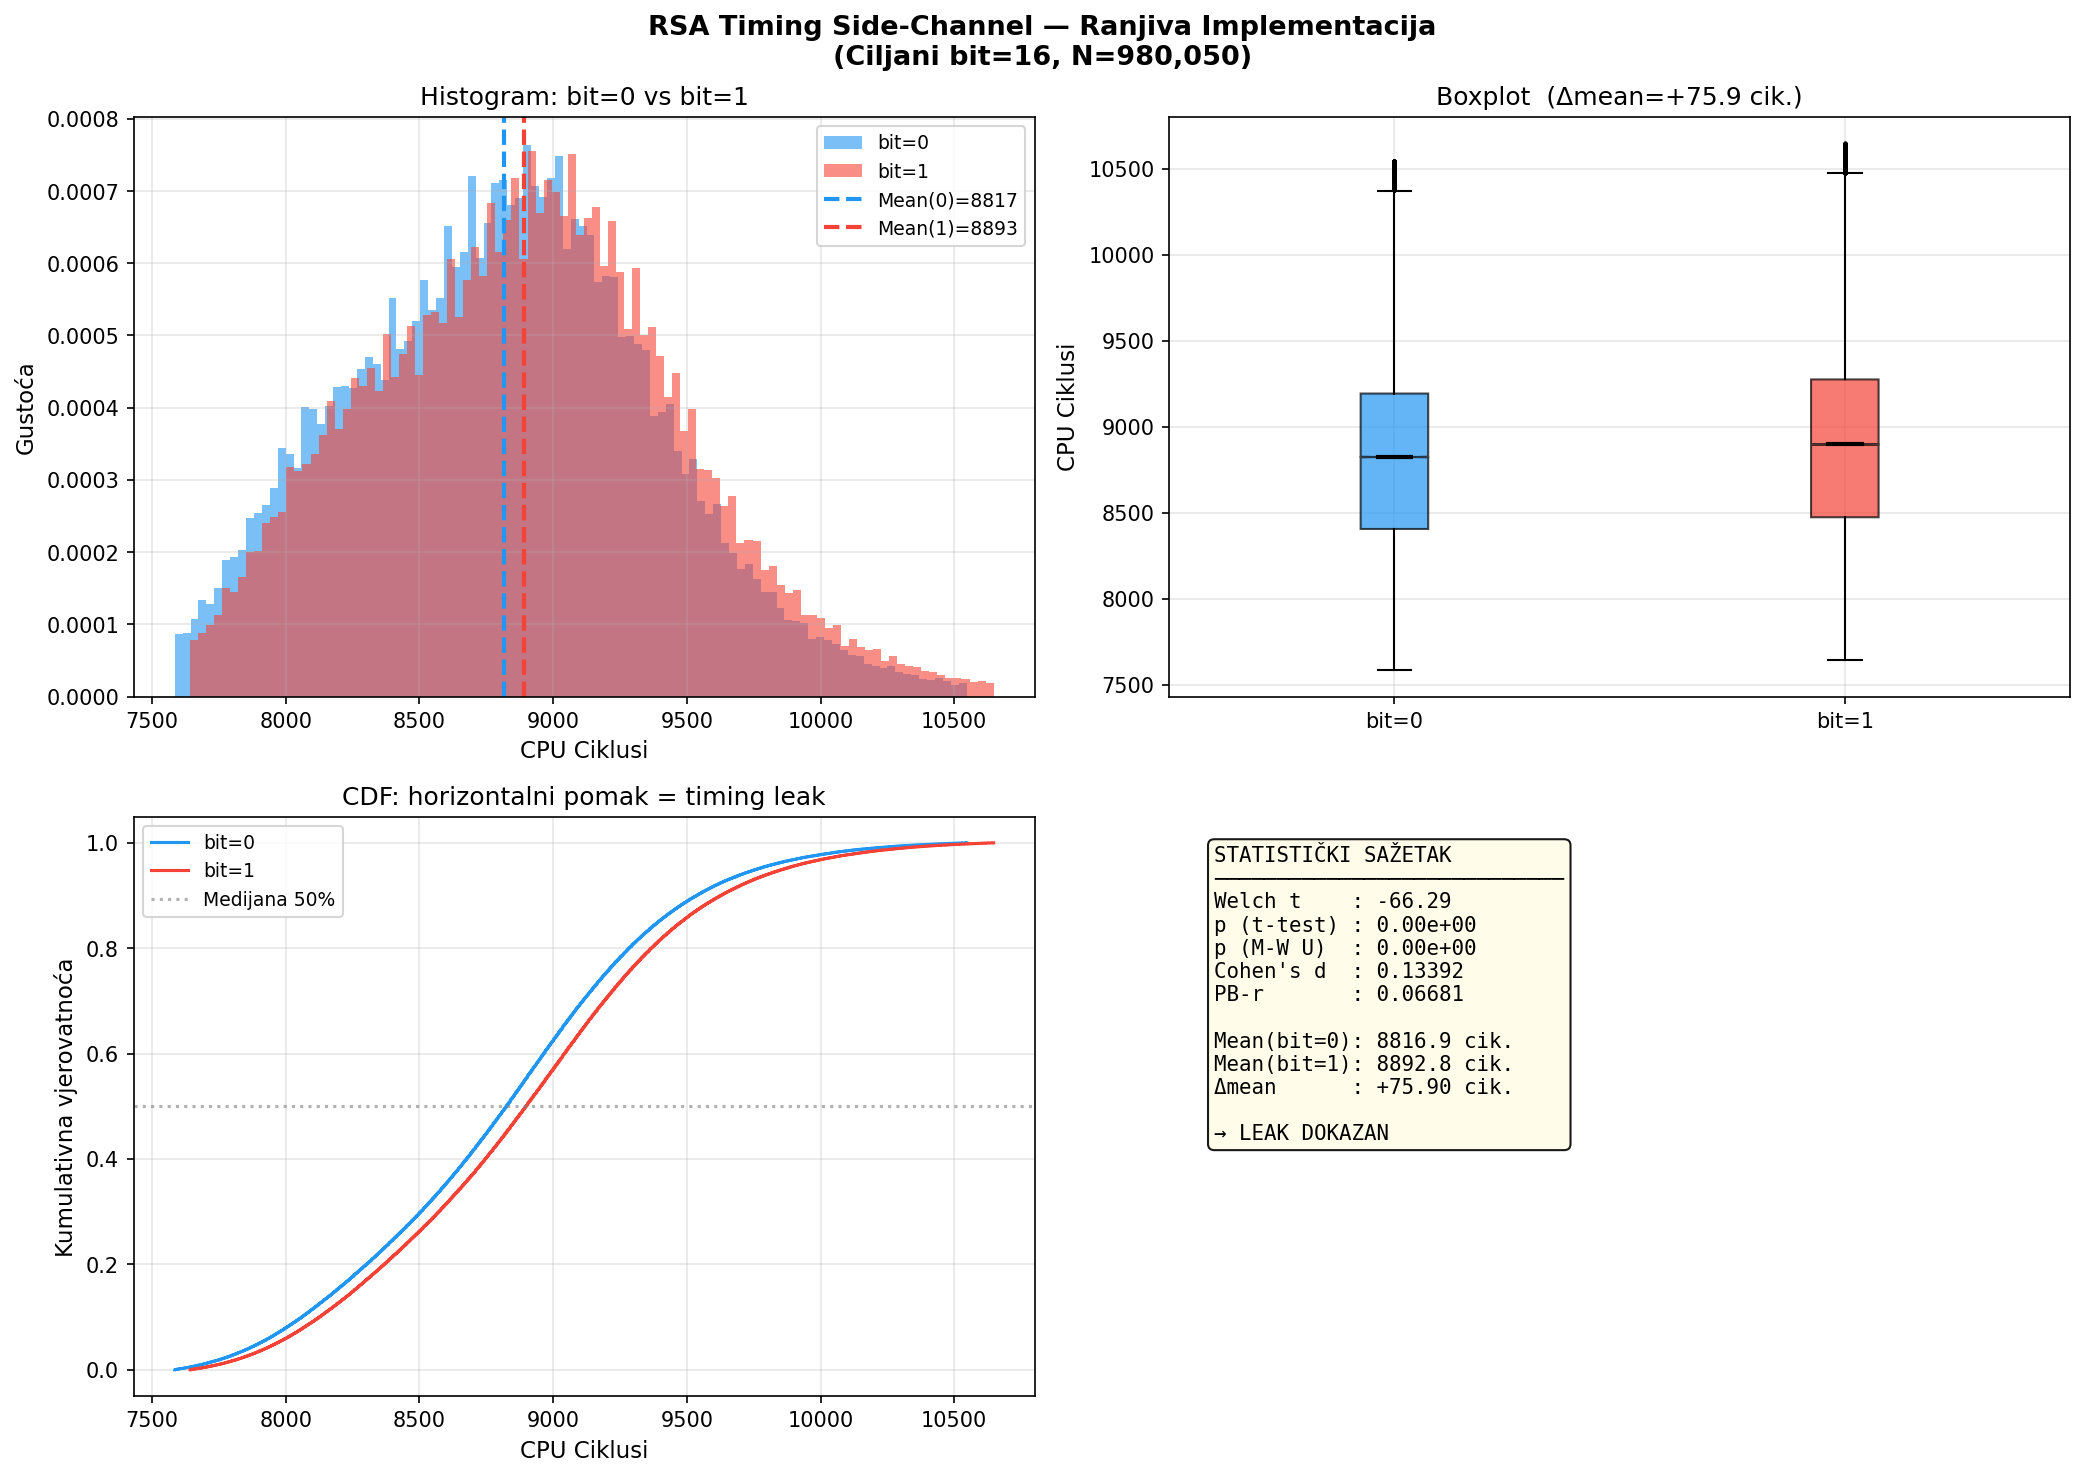
\includegraphics[width=\textwidth]{plot_vulnerable_analysis.png}
\caption{Distribucija trajanja ranjive implementacije: histogram, boxplot i CDF za grupe bit=0 i bit=1.}
\label{fig:vuln_analysis}
\end{figure}

Na slici \ref{fig:vuln_analysis} histogram prikazuje dvije distribucije koje se gotovo potpuno preklapaju, ali s vidljivim horizontalnim pomakom od oko 75 ciklusa. Preklapanje je očekivano s obzirom na mali Cohen-ov $d$: šum (varijansa od cache miss-ova, branch mispredictions i preempcija operativnog sistema) je znatno veći od signala. CDF (kumulativna funkcija distribucije) krivulje jasno ilustruju vremensko curenje: za isti postotak uzoraka, distribucija grupe bit=1 konzistentno zahtijeva veći broj ciklusa. Paralelnost CDF krivulja potvrđuje da je pomak uniforman preko cijele distribucije, a ne lokaliziran na određenom dijelu.

\begin{figure}[H]
\centering
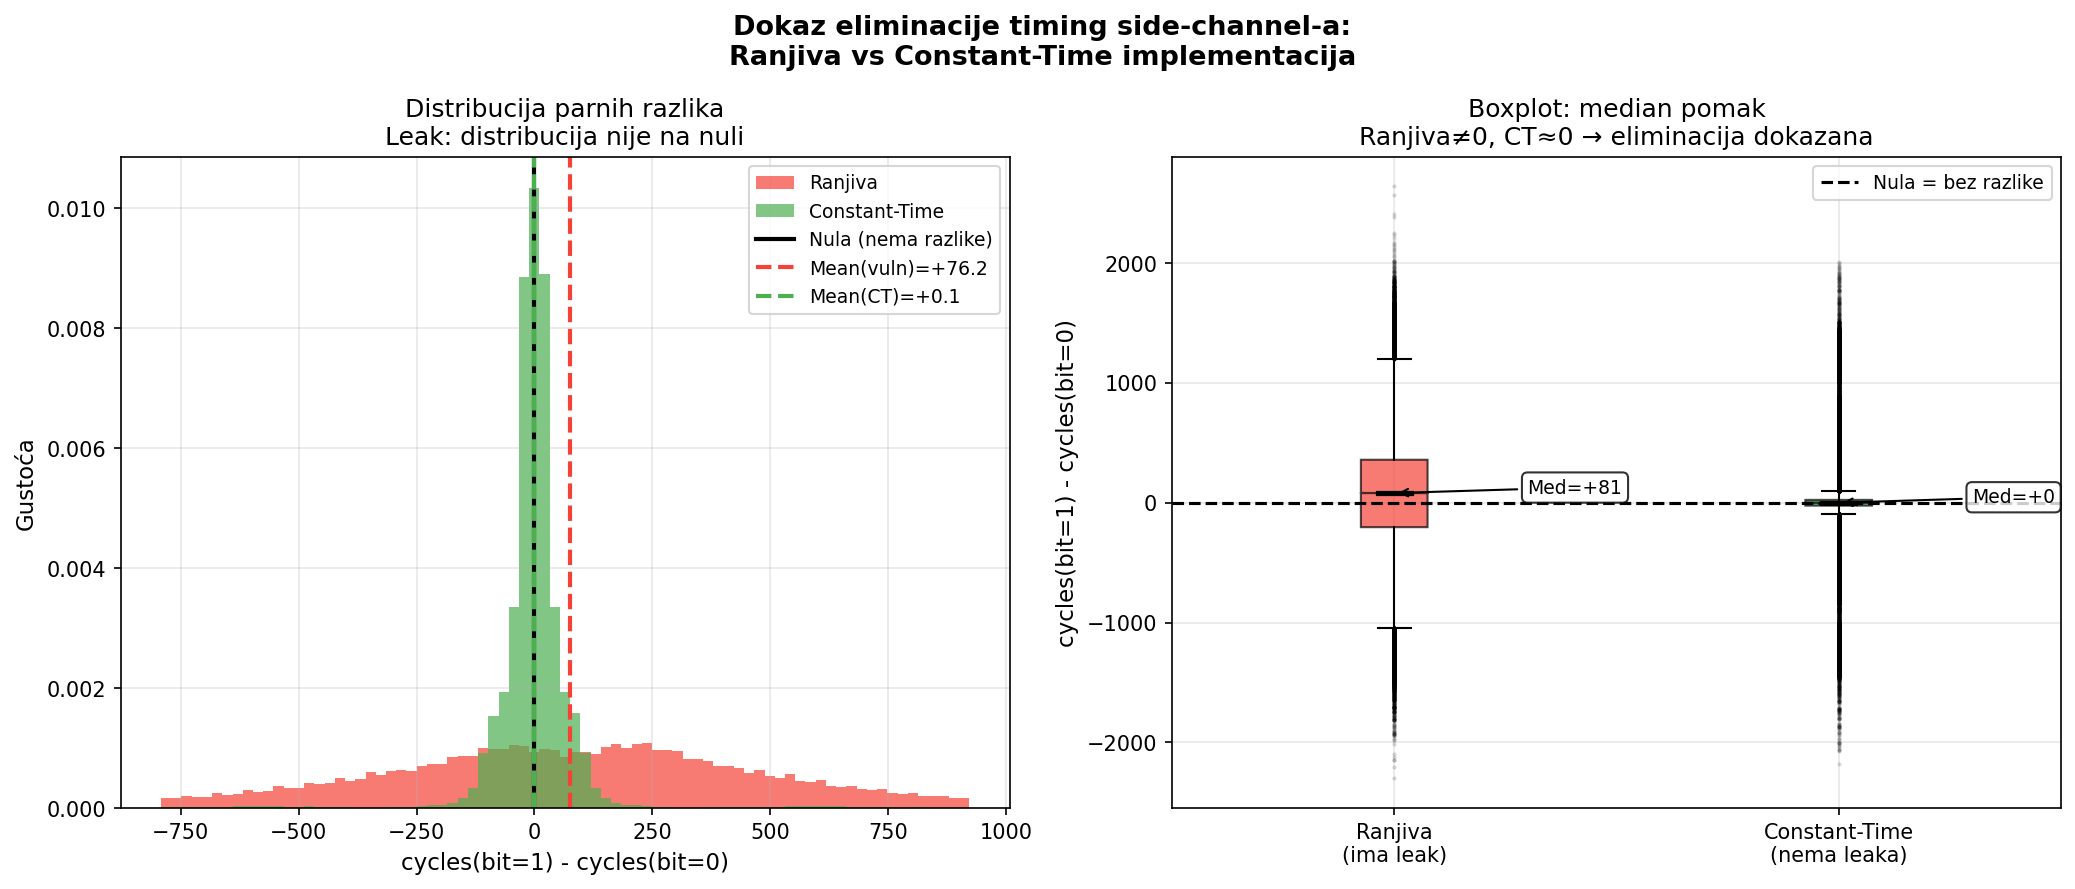
\includegraphics[width=\textwidth]{plot_comparison.png}
\caption{Distribucija parnih razlika trajanja za ranjivu (crvena) i konstantnu vremensku (zelena) implementaciju.}
\label{fig:comparison}
\end{figure}

Slika \ref{fig:comparison} direktno prikazuje distribuciju razlika unutar svakoga para. Za ranjivu implementaciju, centar distribucije je jasno pomaknut udesno od nule (centar na +76 ciklusa), dok za constant-time implementaciju distribucija leži precizno na nuli. Ovo je najintuitivniji vizualni dokaz da implementacija s konstantnim vremenom uspješno eliminiše curenje.

\subsection{Validacija eksperimenta}

Tabela \ref{tab:validation} sumira sedam unaprijed definisanih validacionih kriterija koji zajedno potvrđuju ispravnost eksperimentalnog postupka.

\begin{table}[H]
\centering
\caption{Validacija eksperimenta: svi kriteriji ispunjeni}
\label{tab:validation}
\begin{tabular}{lll}
\toprule
\textbf{Kriterij} & \textbf{Uslov} & \textbf{Rezultat} \\
\midrule
Vremensko curenje postoji & $p_{\text{MW}} < 10^{-10}$ & $< 10^{-50}$ \checkmark \\
T-test značajan & $p < 0{,}01$ & $< 10^{-50}$ \checkmark \\
Efekt mjerljiv & $|d| > 0{,}01$ & $d = 0{,}134$ \checkmark \\
Napad uspješan & tačnost $> 70\%$ & $100\%$ za $K = 2000$ \checkmark \\
CT eliminira leak & $p_{\text{MW}} > 0{,}05$ & $p = 0{,}327$ \checkmark \\
CT bez efekta & $|d| < 0{,}05$ & $d \approx 0{,}000$ \checkmark \\
CT napad neuspješan & tačnost $< 60\%$ & $\approx 50\%$ \checkmark \\
\bottomrule
\end{tabular}
\end{table}

Ispunjenje svih sedam kriterija potvrđuje da eksperimentalni postupak ispravno detektuje vremensko curenje kada postoji, i ispravno ne detektuje ništa kada ga nema. Ovo isključuje mogućnost da su rezultati posljedica metodološke greške.

% ---------------------------------------------------------------

\section{Eksperiment 2: Napad sa usrednjavanjem}
\label{sec:exp2}

\subsection{Metodologija}

Eksperiment 1 dokazuje da vremensko curenje postoji, ali postavlja se pitanje: može li napadač praktično iskoristiti signal od samo 76 ciklusa u šumu od 567 ciklusa za pogađanje vrijednosti tajnog bita? Eksperiment odgovara na ovo pitanje tako što demonstrira da usrednjavanje više mjerenja ignoriše šum i izvlači signal.

Za svaki nivo usrednjavanja K, napadač izvodi sljedeći postupak: (1) procjenjuje optimalni prag iz prve polovice podataka, (2) formira K nasumičnih mjerenja iz testnog skupa i računa njihovu sredinu, te (3) klasificira usrednjeni rezultat pravilom praga: ako je sredina iznad praga, proglašava bit=1, inače bit=0.

Teorijski minimalan K za postizanje 95\% tačnosti izvodi se iz odnosa signala i šuma. Za SNR $= d = 0{,}134$ i faktor pouzdanosti $r = 2$ (koji odgovara 95\% jednosmjernoj pouzdanosti, jednačina \ref{eq:kmin} daje $K_{\min} = (r/\text{SNR})^2 = (2/0{,}134)^2 \approx 223$. Intuicija iza ove formule je da standardna devijacija sredine od K mjerenja je $\sigma/\sqrt{K}$, pa sa dovoljno velikim K sredina postaje dovoljno precizna da signal od 76 ciklusa bude jasno odvojen od šuma.

\subsection{Rezultati}

\begin{table}[H]
\centering
\caption{Tačnost timing napada sa usrednjavajem u funkciji broja usrednjenih mjerenja K}
\label{tab:averaging}
\begin{tabular}{rrrr}
\toprule
\textbf{K} & \textbf{Tačnost (ranjiva)} & \textbf{95\% CI} & \textbf{Tačnost (CT)} \\
\midrule
1      & 53{,}4\% & [51{,}9\%, 54{,}9\%] & 50{,}2\% \\
10     & 57{,}8\% & [56{,}3\%, 59{,}3\%] & 50{,}0\% \\
100    & 74{,}6\% & [73{,}2\%, 75{,}9\%] & 50{,}9\% \\
500    & 92{,}4\% & [90{,}6\%, 93{,}9\%] & 50{,}9\% \\
1000   & 97{,}6\% & [95{,}8\%, 98{,}6\%] & 52{,}2\% \\
2000   & 100{,}0\% & [98{,}4\%, 100{,}0\%] & 43{,}9\% \\
5000   & 100{,}0\% & [96{,}2\%, 100{,}0\%] & 51{,}0\% \\
\bottomrule
\end{tabular}
\end{table}

\begin{figure}[H]
\centering
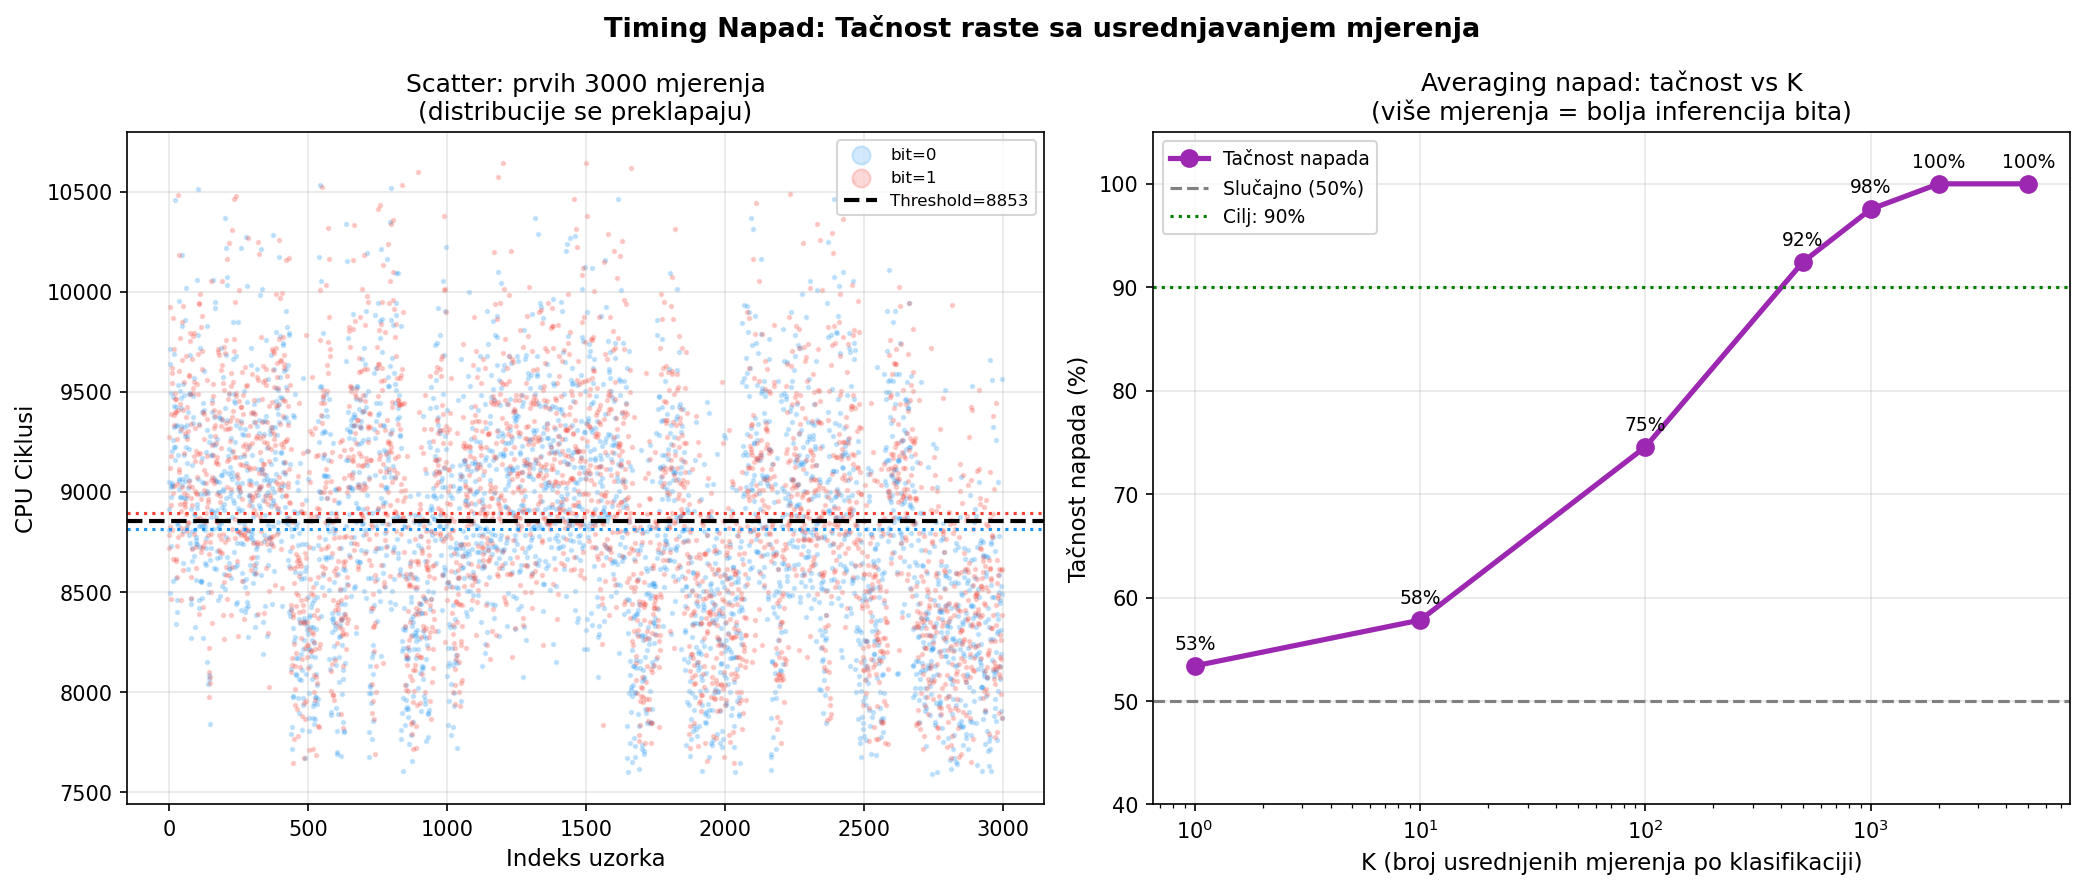
\includegraphics[width=\textwidth]{plot_inference_attack.png}
\caption{Dijagram raspršenja (\textit{scatter plot}) mjerenja (lijevo) i tačnost u funkciji K (desno).}
\label{fig:inference}
\end{figure}

Slika \ref{fig:inference} prikazuje rasipanje pojedinačnih mjerenja (lijevo) i rast tačnosti s povećanjem K (desno). Rezultati potvrđuju teorijsko predviđanje. Sa jednim mjerenjem ($K=1$), napadač pogađa tek 53{,}4\%, jedva iznad slučajnog pogađanja od 50\%, jer je signal zakopan u šumu. Sa $K = 100$, tačnost raste na 74{,}6\%, što je blizu teorijskog $K_{\min} = 223$ za 95\%. Sa $K = 500$ napadač postiže 92{,}4\%, a sa $K = 2000$ dostiže savršenih 100\%.

Fizičko objašnjenje: za $K = 2000$, standardna devijacija sredine iznosi $\sigma_{2000} = 567/\sqrt{2000} \approx 12{,}7$ ciklusa. Signal od 76 ciklusa je sada šest puta veći od šuma sredine, što čini pogrešnu klasifikaciju praktično nemogućom.

Za implementaciju s konstantnim vremenom tačnost napada ostaje u opsegu 44--52\% za sve vrijednosti K, što je konzistentno s odsustvom vremenskog curenja. Vrijednost od 43{,}9\% za $K = 2000$ je statističko odstupanje; 95\% interval povjerenja za slučajno pogađanje s 200--500 test blokova obuhvata ovaj raspon.

\subsection{Osjetljivost na veličinu uzorka}

Tabela \ref{tab:sensitivity} prikazuje kako se statistička značajnost i tačnost napada mijenjaju kada se koristi samo podskup ukupnih podataka. Ova analiza odgovara na pitanje: koliko mjerenja napadač minimalno treba prikupiti?
\begin{table}[H]
\centering
\caption{Osjetljivost na veličinu uzorka: p-vrijednost i tačnost napada}
\label{tab:sensitivity}
\begin{tabular}{rrrr}
\toprule
\textbf{N uzoraka} & \textbf{p-vrijednost} & \textbf{Značajno?} & \textbf{Tačnost ($K = 100$)} \\
\midrule
100       & 4{,}53e-02  & Da    & N/A \\
500       & 1{,}76e-02  & Da    & 90{,}0\% \\
1\,000    & 2{,}65e-07  & Da    & 90{,}0\% \\
2\,000    & 3{,}85e-07  & Da    & 85{,}0\% \\
5\,000    & 1{,}68e-12  & Da    & 75{,}0\% \\
10\,000   & 6{,}14e-17  & Da    & 70{,}5\% \\
50\,000   & 7{,}81e-112 & Da    & 73{,}6\% \\
100\,000  & 3{,}50e-198 & Da    & 76{,}9\% \\
\bottomrule
\end{tabular}
\end{table}

Za $N = 100$, usrednjavanje sa $K = 100$ nije moguće jer ukupan broj uzoraka nije dovoljan za formiranje nezavisnih blokova, pa je tačnost označena kao N/A. Najmanji N za postizanje statističke značajnosti ($p < 0{,}05$) iznosi $N = 100$ ($p = 4{,}53 \times 10^{-2}$). Čak i sa samo 100 uzoraka timing leak je na granici statističke vidljivosti, uprkos tome što power analiza za 80\% snagu predviđa $N_{\min} = 438$. Ovo sugeriše da je stvarna veličina efekta u ovom poduzorku bila nešto veća od ukupnog prosjeka.

Naizgled paradoksalan pad tačnosti napada za veće $N$ (npr. 90\% za $N=500$ naspram 70{,}5\% za $N=10\,000$ uz $K=100$) objašnjava se nestabilnošću procjene pri malom broju test blokova. Za $N=500$ i $K=100$ postoji samo 5 nezavisnih blokova (svaki od 100 mjerenja), pa jedan ili dva sretna bloka značajno utječu na procijenjenu tačnost. Za veće $N$, broj blokova raste i procjena konvergira ka stvarnoj tačnosti od približno 75\% za $K=100$, što odgovara teorijskom predviđanju za SNR $= 0{,}134$ i $K$ daleko ispod $K_{\min} = 223$.

\begin{figure}[H]
\centering
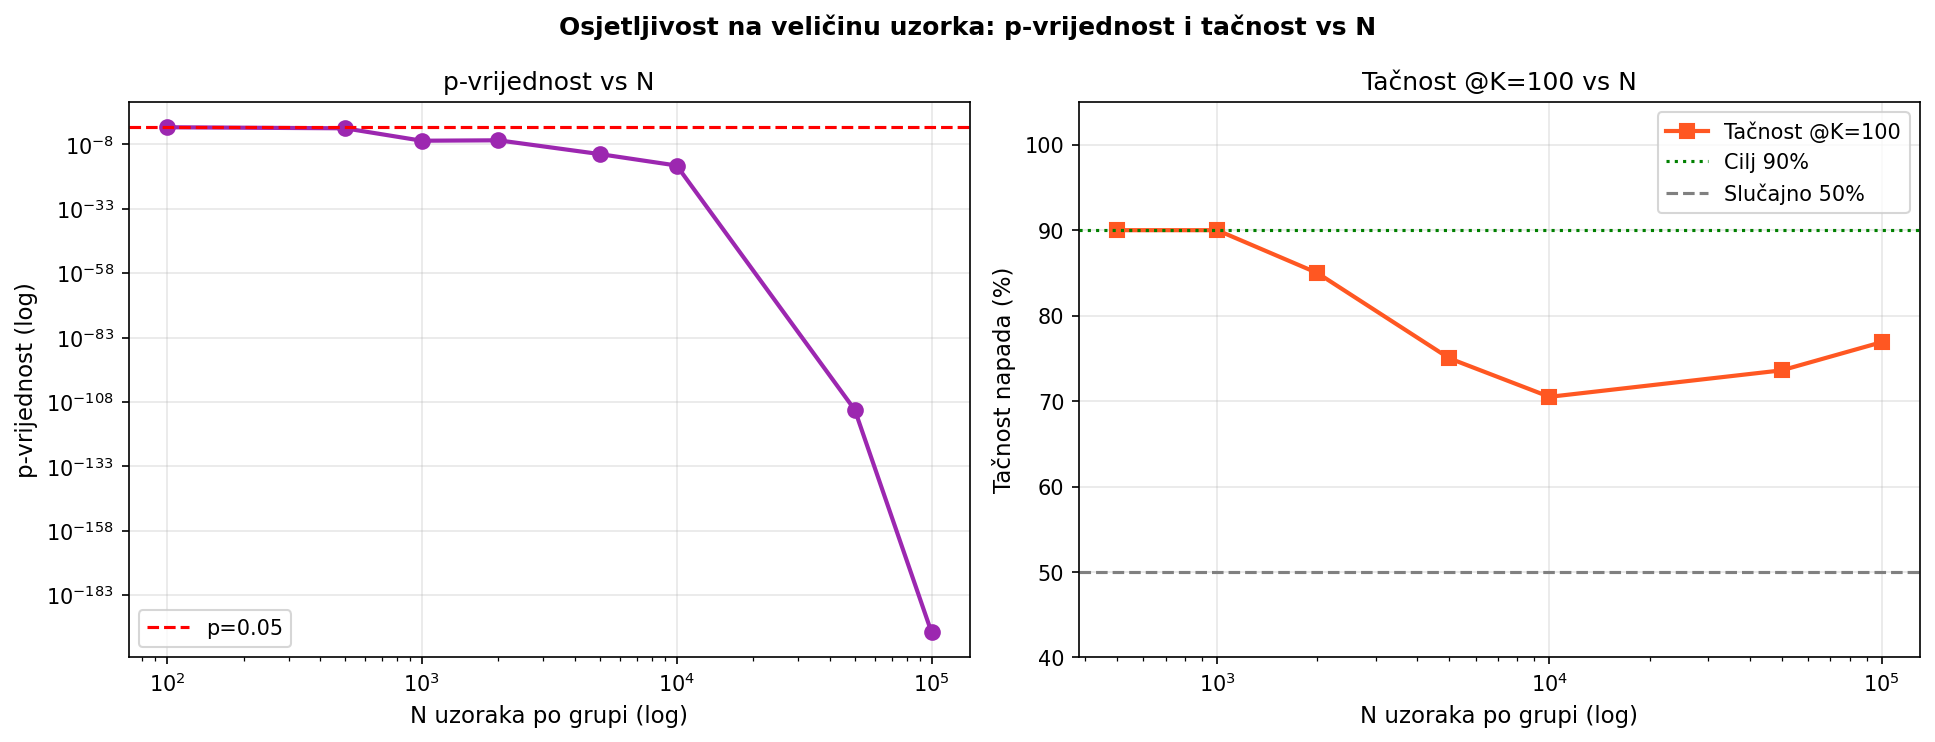
\includegraphics[width=\textwidth]{plot_sample_sensitivity.png}
\caption{Osjetljivost napada na veličinu uzorka: tačnost u funkciji $N$ za $K = 100$.}
\label{fig:sample_sensitivity}
\end{figure}

% ---------------------------------------------------------------

\section{Eksperiment 3: Slijepa rekonstrukcija 64-bitnog privatnog ključa}
\label{sec:exp3}

\subsection{Metodologija}

Eksperimenti 1 i 2 pokazuju da napadač može pouzdano odrediti vrijednost jednog bita. Eksperiment 3 primjenjuje isti princip na svih 64 bita privatnog ključa i rekonstruiše cijeli ključ, uz jedno ključno obilježje: napadački kod nikada ne vidi tajni ključ.

Tajni ključ generisan je nasumično iz \texttt{/dev/urandom} i pohranjen unutar zasebnog modula kome napadač nema direktan pristup (sekcija~\ref{sec:key_recon}). Za svaki bit napadač pita taj modul koliko dugo traje eksponencijacija s originalnim ključem i koliko bi trajala da je samo taj jedan bit obrnut. Iz razlike tih trajanja zaključuje koja je bila izvorna vrijednost bita. Ovaj postupak se ponavlja za sva 64 bita, sa $K = 5000$ mjerenja po bitu radi pouzdanosti. Tek na samom kraju, radi provjere tačnosti, modul otkriva tajni ključ.

\subsection{Rezultati}

\begin{table}[H]
\centering
\caption{Rezultati slijepe rekonstrukcije 64-bitnog ključa}
\label{tab:key_recon}
\begin{tabular}{ll}
\toprule
\textbf{Metrika} & \textbf{Vrijednost} \\
\midrule
Tajni ključ (nasumičan, \texttt{/dev/urandom}) & \texttt{0xAB568018B673C14C} \\
Rekonstruisani ključ                           & \texttt{0xAB568018B673C14C} \\
XOR razlika                                    & \texttt{0x0000000000000000} \\
Tačni biti                                     & 64 / 64 (100{,}0\%) \\
K po bitu                                      & 5\,000 \\
Mean $|\Delta|$                                & 73{,}1 ciklusa \\
Mean $\Delta$ (bit=1 pozicije)                 & $+$54{,}6 ciklusa \\
Mean $\Delta$ (bit=0 pozicije)                 & $-$87{,}4 ciklusa \\
\bottomrule
\end{tabular}
\end{table}

\begin{figure}[H]
\centering
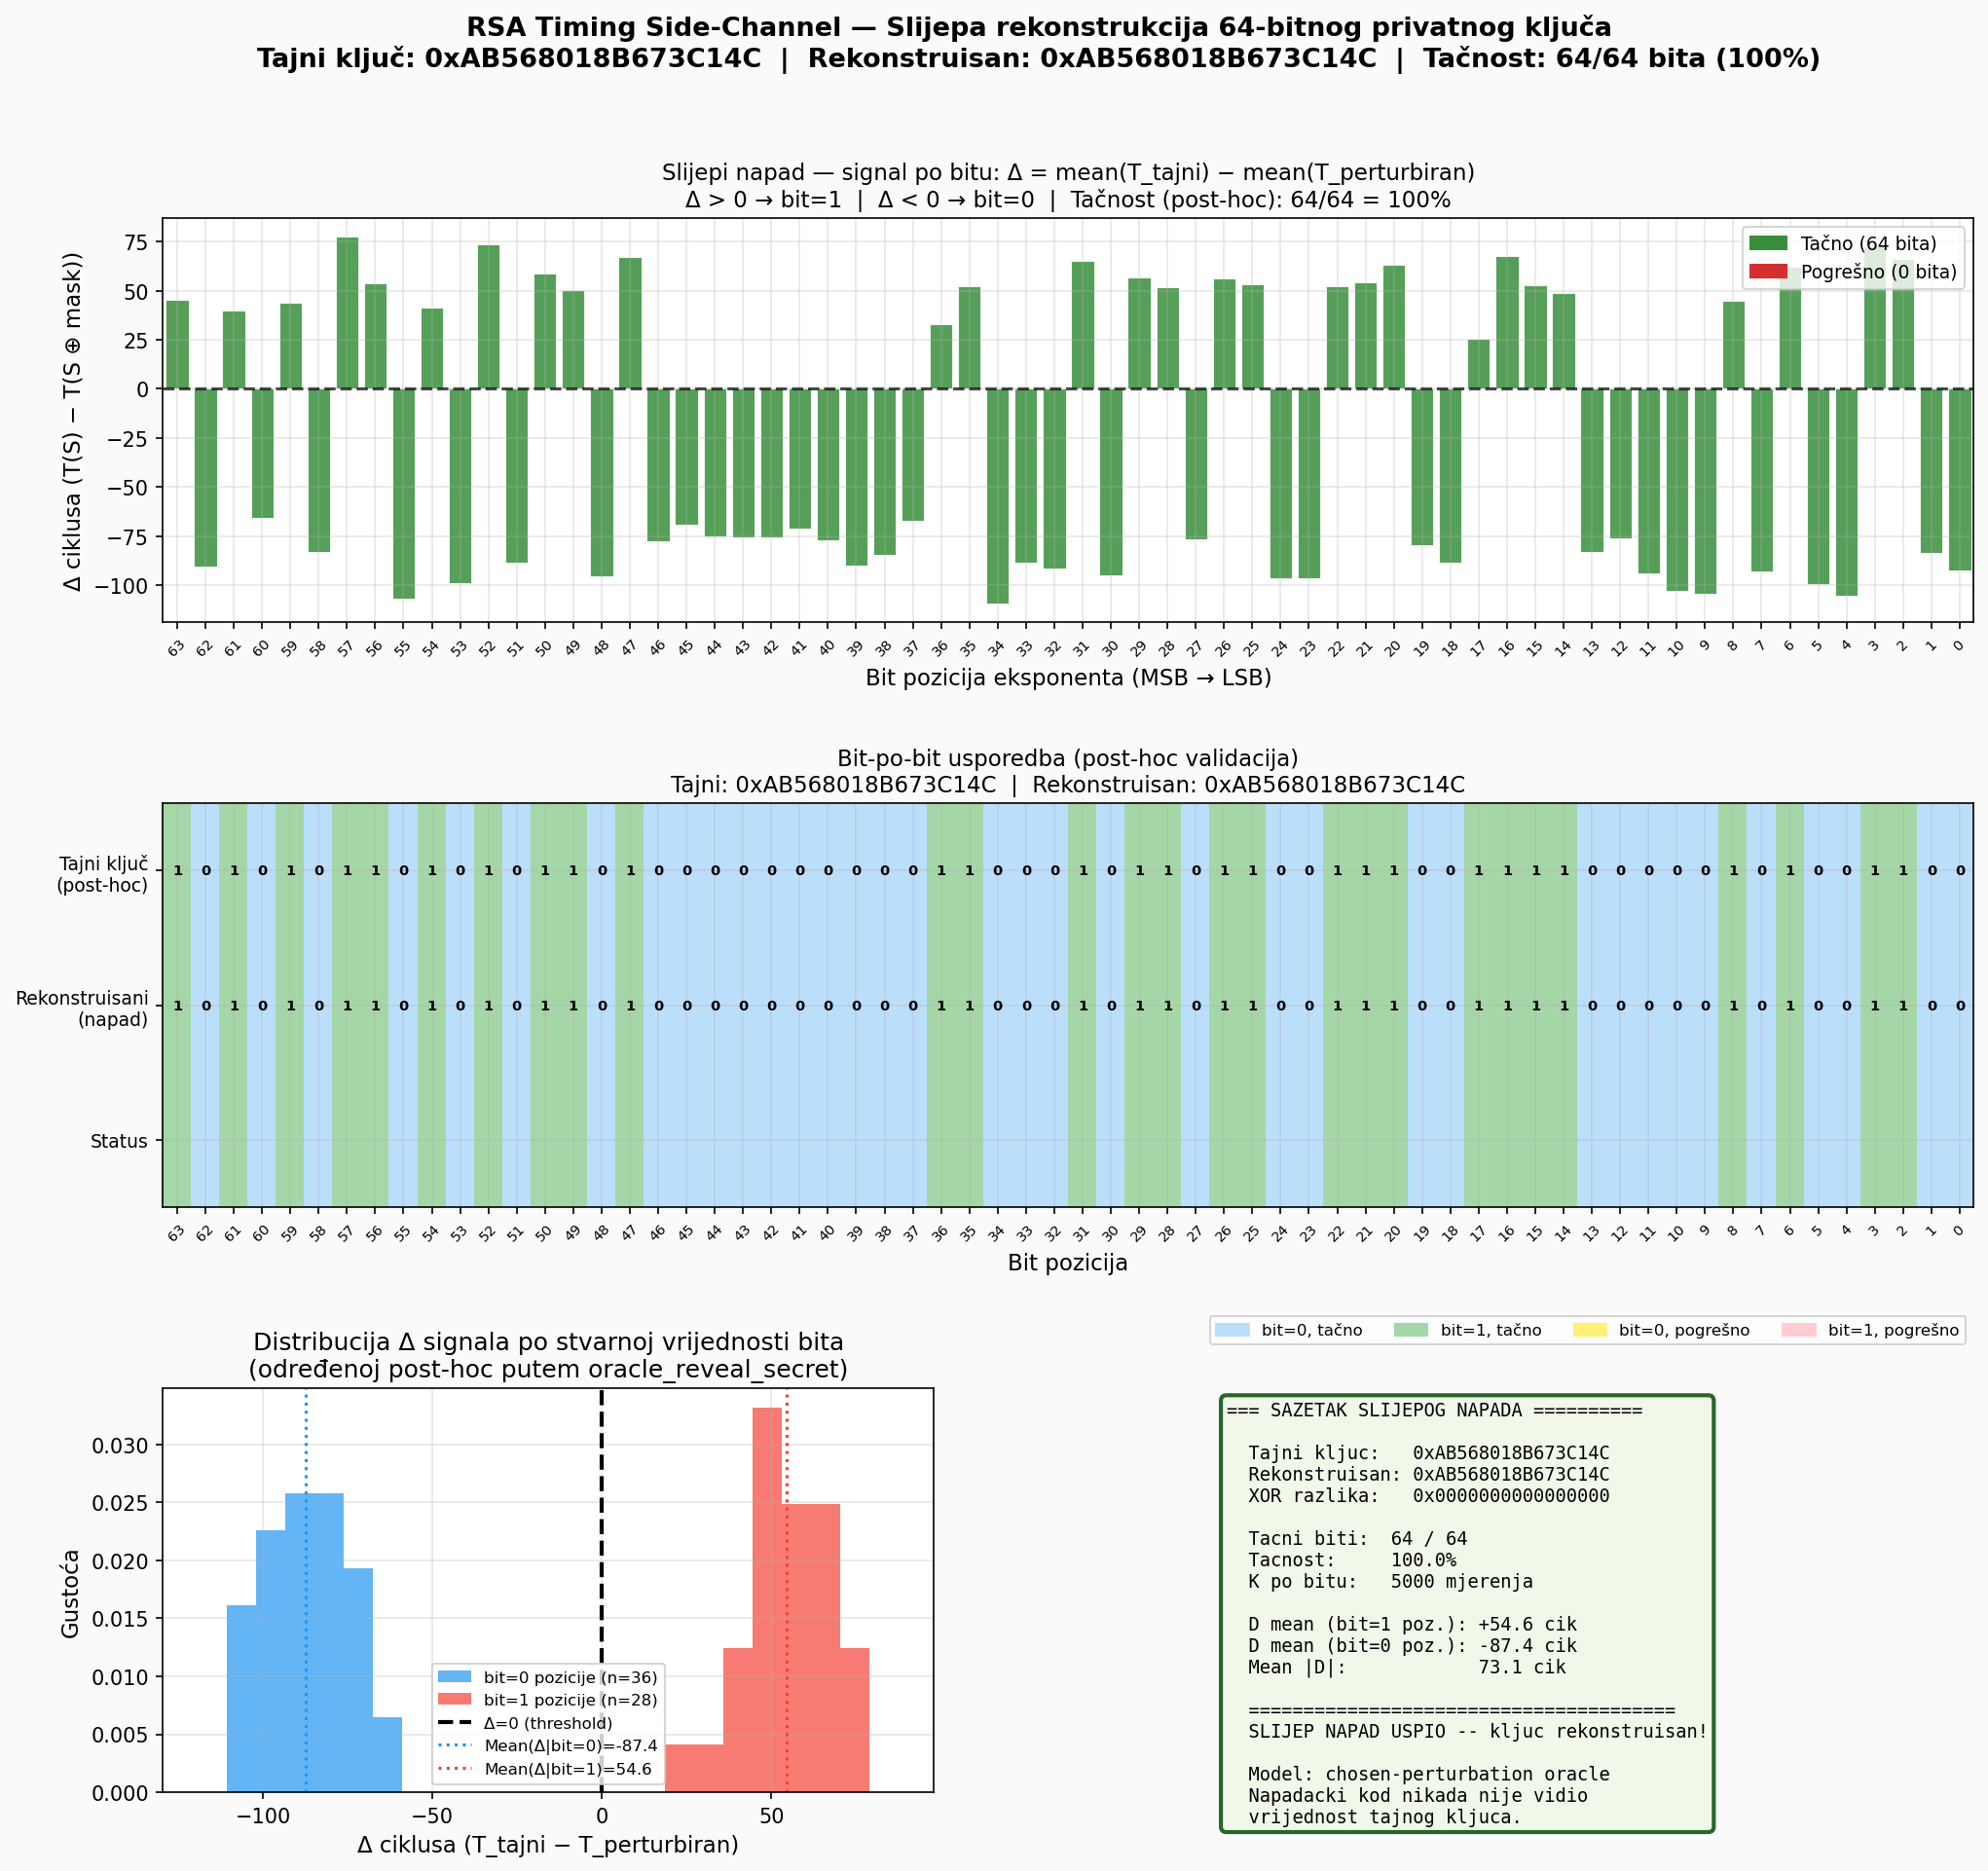
\includegraphics[width=\textwidth]{plot_key_reconstruction_blind.png}
\caption{Gornji panel: timing razlika $\Delta$ za svaki od 64 bita (pozitivna vrijednost = bit=1, negativna = bit=0). Srednji panel: toplotna mapa rekonstruisanog i stvarnog ključa. Donji panel: distribucija svih $\Delta$ vrijednosti}
\label{fig:key_recon}
\end{figure}

Kao što se vidi na slici \ref{fig:key_recon}, svih 64 bita nasumičnog tajnog ključa su tačno rekonstruisani. Timing razlika $\Delta$ je konzistentna i jasno odvojena po predznaku na svim pozicijama: pozicije gdje je tajni bit 1 daju pozitivan $\Delta$ (prosjek $+54{,}6$ ciklusa), a pozicije gdje je bit 0 daju negativan $\Delta$ (prosjek $-87{,}4$ ciklusa). Predznak $\Delta$ direktno otkriva vrijednost bita jer obrtanje bita iz 1 u 0 uklanja jedno množenje i skraćuje trajanje, dok obrtanje iz 0 u 1 dodaje množenje i produžava ga.

Veličina signala varira od pozicije do pozicije: najslabija razlika bila je 25{,}3 ciklusa (bit 17), a najjača 109{,}2 ciklusa (bit 34). Ova varijacija je normalna i odgovara rezultatima Eksperimenta 4. Ni za jedan bit nisu bila potrebna ponovna mjerenja: najmanji $|t|$-statistik iznosio je 8{,}3, daleko iznad praga od 2{,}5 koji bi aktivirao drugi prolaz.

Rekonstrukcija je potpuno zasnovana na timing mjerenjima i napadački kod u nijednom trenutku nije pristupio vrijednosti tajnog ključa. Ovo odgovara realnom napadu: server drži privatni ključ, a napadač ga može jedino posredno "posmatrati" kroz razlike u trajanju odgovora.

% ---------------------------------------------------------------

\section{Eksperiment 4: Analiza pozicije bita}

\subsection{Motivacija i metodologija}

Eksperimenti 1 i 2 ciljaju fiksiranu poziciju bita (bit 16), a Eksperiment 3 primjenjuje napad na svih 64 bita. Prirodno pitanje je: da li je vremensko curenje sistemska osobina koja važi za svaku poziciju, ili postoje pozicije gdje je signal slabiji? Odgovor na ovo pitanje je ključan jer napad rekonstrukcije ključa pretpostavlja da svaki bit nezavisno daje mjerljiv signal.

Eksperiment testira svaku od 64 pozicija bita nezavisno, sa 10\,000 uzoraka po poziciji, i za svaku izračunava Welch-ov t-test i Cohen-ov $d$.

\subsection{Rezultati}

\begin{table}[H]
\centering
\caption{Multi-bit sweep: ukupni rezultati}
\label{tab:sweep_summary}
\begin{tabular}{ll}
\toprule
\textbf{Metrika} & \textbf{Vrijednost} \\
\midrule
Statistički značajnih pozicija & 64 / 64 (100\%) \\
Mean $\Delta$ po svim bitovima & +75{,}67 ciklusa \\
Std $\Delta$ & 7{,}07 ciklusa \\
One-sample t-test ($H_0$: mean $\Delta = 0$) & $t = 84{,}993$,\ $p = 1{,}027 \times 10^{-66}$ \\
\bottomrule
\end{tabular}
\end{table}

\begin{figure}[H]
\centering
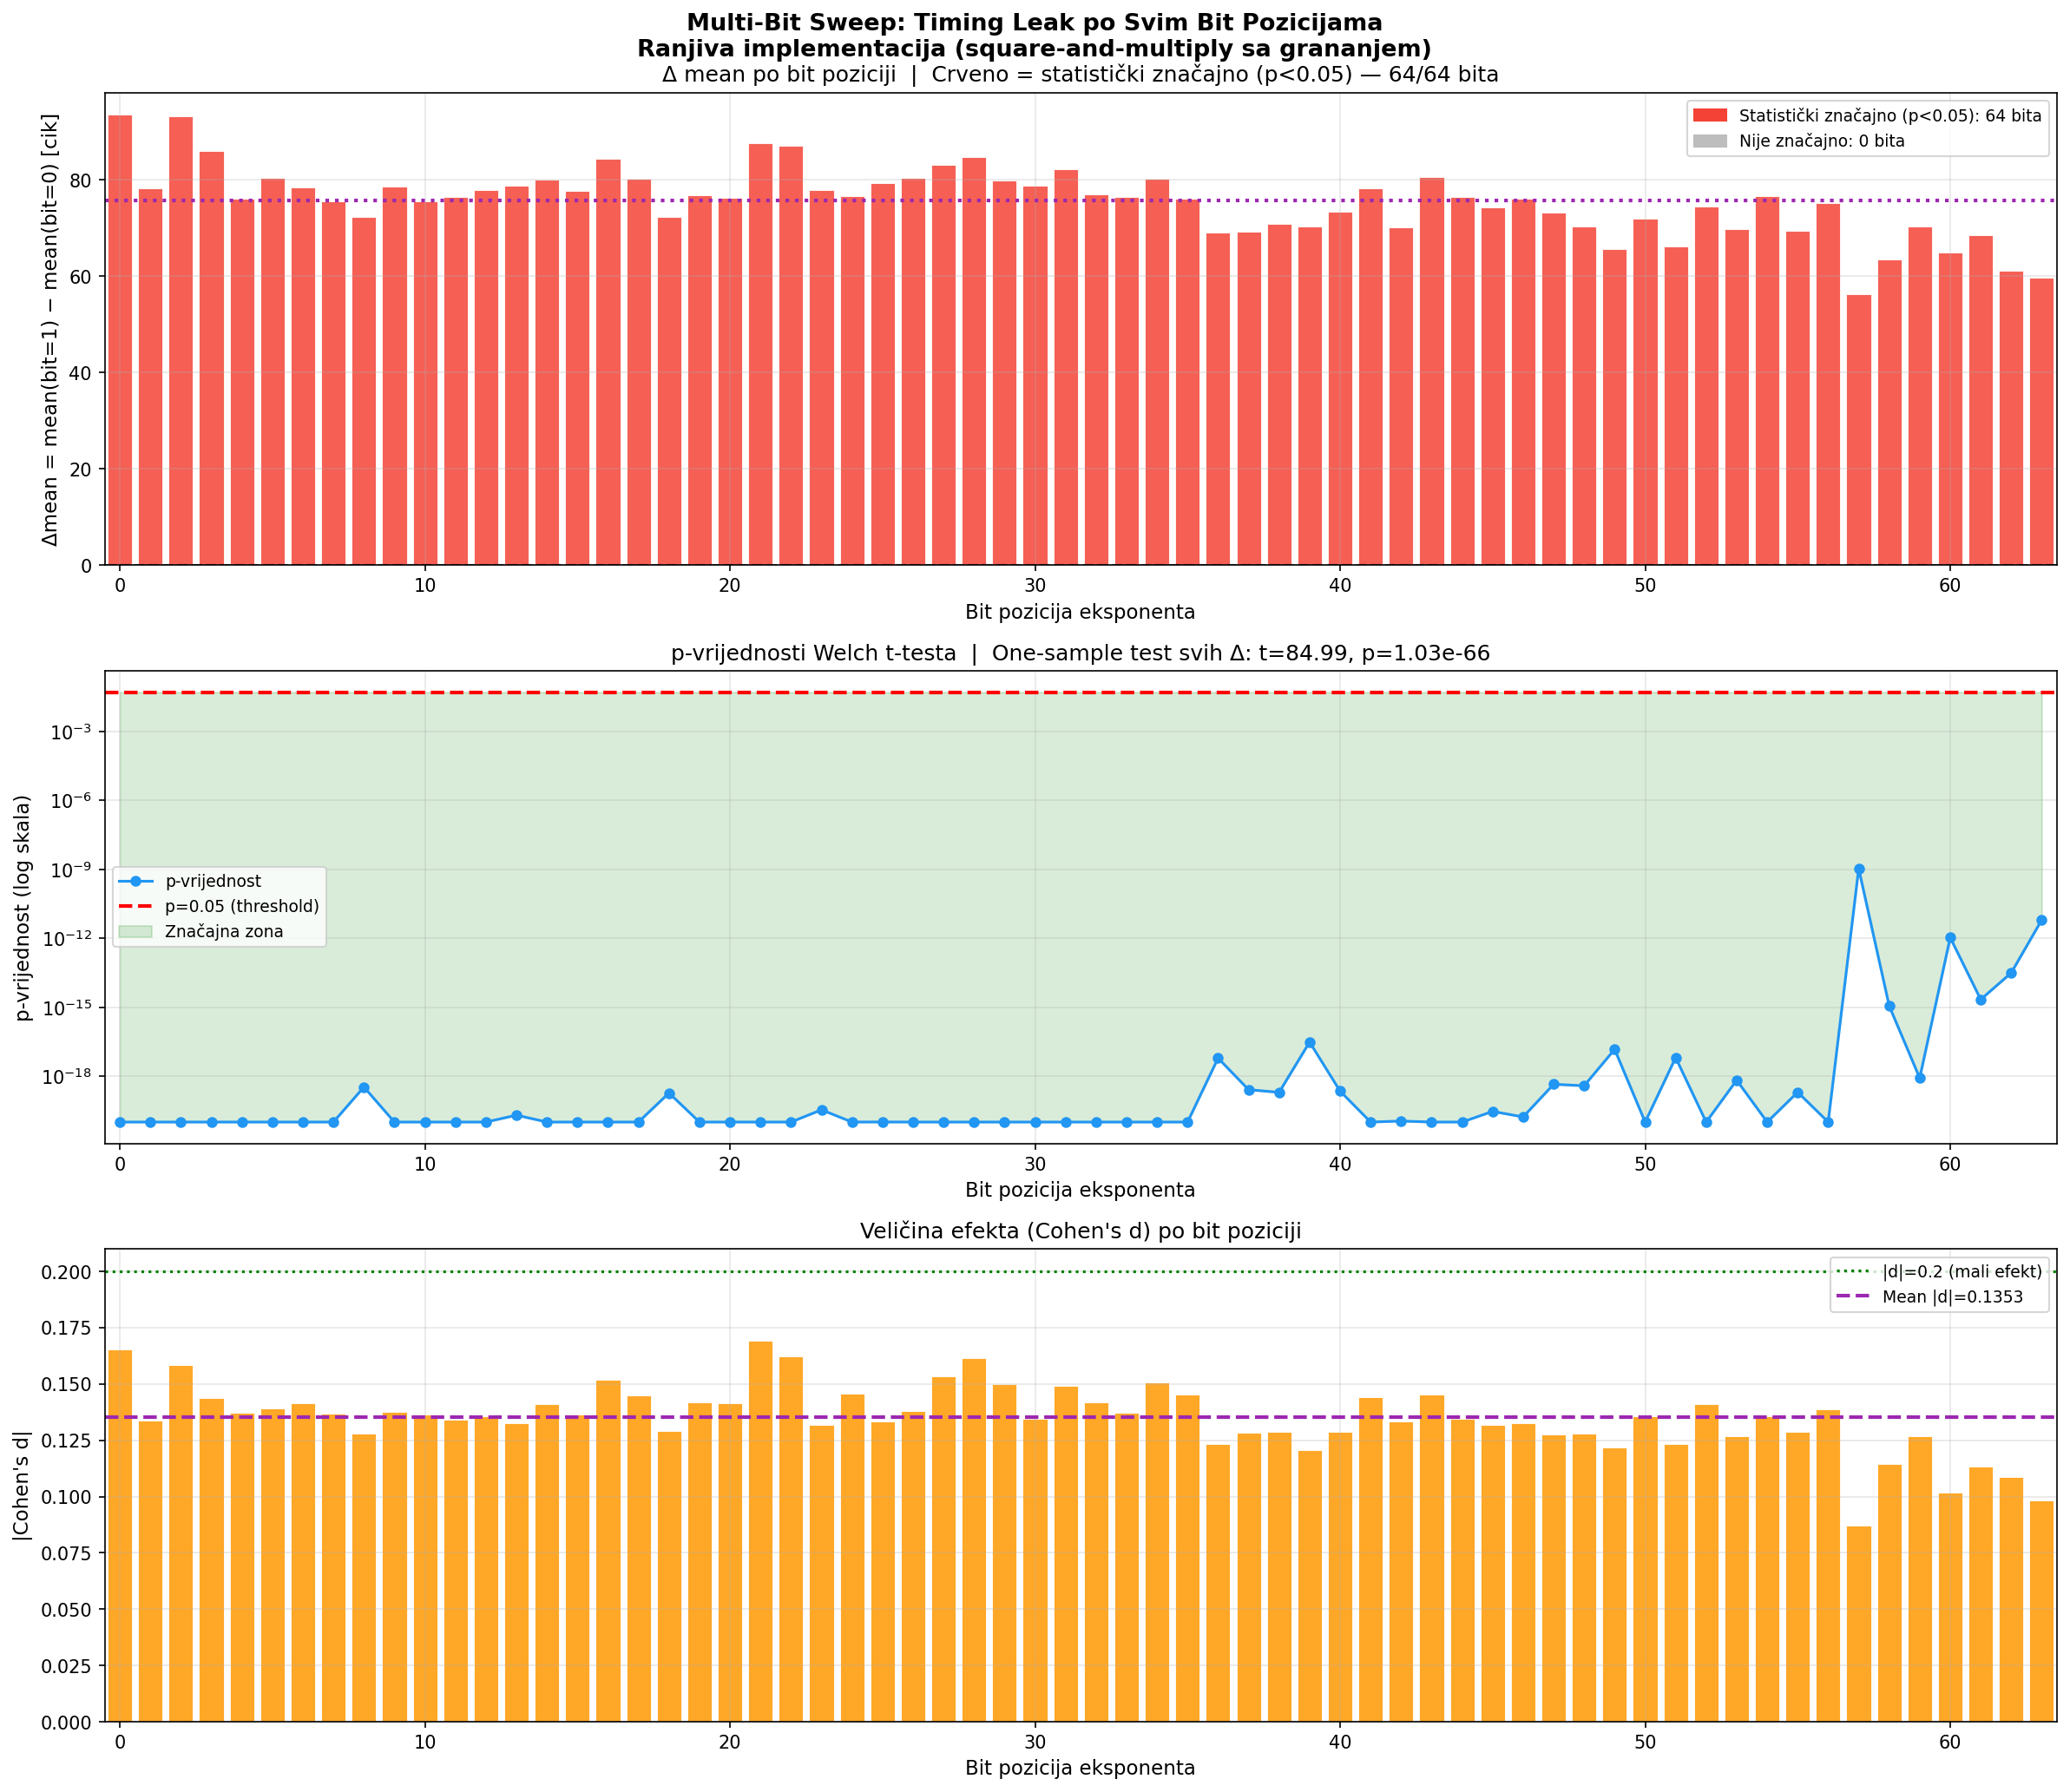
\includegraphics[width=\textwidth]{plot_multi_bit_sweep.png}
\caption{Timing razlika $\Delta$ po poziciji bita eksponenta sa 95\% intervalima povjerenja.}
\label{fig:sweep}
\end{figure}

Svih 64 pozicija bita pokazuju statistički značajnu vremensku razliku ($p < 10^{-9}$ za svaku poziciju pojedinačno). Prosječna razlika $\Delta$ kreće se od $+56{,}22$ ciklusa (bit 57) do $+93{,}49$ ciklusa (bit 0), sa ukupnom standardnom devijacijom od 7{,}07 ciklusa između pozicija.
\\

Varijacija $\Delta$ po poziciji (od 56 do 93 ciklusa) nije sistematski trend nego kontekstualni šum: svaka iteracija petlje zatekne različito stanje branch prediktora i cache memorije ovisno o tome koji su se bitovi izvršili ranije, što uvodi slučajnu varijabilnost u izmjerenu razliku. Minimalna vrijednost na bitu 57 i maksimalna na bitu 0 su primjer te slučajnosti i ne postoji krivulja koja pada ili raste s pozicijom. Za realni 2048-bitni ključ slika bi izgledala isto: oko 2048 tačaka grupisanih oko iste srednje vrijednosti (~75 ciklusa) s jednakom slučajnom rasutošću. Standardna devijacija od samo 7{,}07 ciklusa (naspram srednje vrijednosti od 75{,}67) potvrđuje visoku konzistentnost signala bez obzira na poziciju.
\\

One-sample t-test svih 64 delta vrijednosti daje $t = 84{,}993$ ($p = 1{,}027 \times 10^{-66}$), čime se definitivno odbacuje hipoteza da je prosječna razlika jednaka nuli. Ovaj rezultat potvrđuje da vremensko curenje nije nastalo zbog jedne bit pozicije, već je osobina ranjive square-and-multiply implementacije: svaki bit eksponenta nezavisno doprinosi mjerljivoj vremenskoj razlici.

% ---------------------------------------------------------------

\section{Eksperiment 5: Utjecaj kompajlerskih optimizacija}
\label{sec:compiler_exp}

\subsection{Motivacija}

U sekciji \ref{sec:vuln_impl} navedeno je da ranjiva implementacija koristi \texttt{optimize("O0")} atribut koji isključuje optimizacije. Postavlja se praktično pitanje: može li kompajler s višim nivoom optimizacije automatski eliminisati timing leak, na primjer transformacijom uslovnog grananja (\texttt{if}) u instrukciju uslovnog pomaka (\texttt{CMOV}) koja se izvršava u konstantnom vremenu? Ako bi to bio slučaj, programeri bi se mogli osloniti na kompajler umjesto na eksplicitne kontramjere.

Ovaj eksperiment testira pet varijanti iste ranjive implementacije kompajlirane s različitim optimizacijskim nivoima i provjerava generisani asemblerski kod.

\subsection{Rezultati}

\begin{table}[H]
\centering
\caption{Timing leak po nivoima kompajlerske optimizacije}
\label{tab:compiler}
\begin{tabular}{llrrrrl}
\toprule
\textbf{Varijanta} & \textbf{Opt.} & \textbf{Atribut} & \textbf{$\Delta$ mean} & \textbf{p-vrijednost} & \textbf{Cohen-ov $d$} & \textbf{Assembly} \\
\midrule
O0       & \texttt{-O0} & Ne  & +77{,}29 & $< 10^{-50}$ & 0{,}136 & branch \\
O1       & \texttt{-O1} & Ne  & +72{,}01 & $< 10^{-50}$ & 0{,}267 & branch \\
O2       & \texttt{-O2} & Ne  & +71{,}73 & $< 10^{-50}$ & 0{,}267 & branch \\
O3       & \texttt{-O3} & Ne  & +71{,}83 & $< 10^{-50}$ & 0{,}267 & branch \\
O2+attr  & \texttt{-O2} & Da  & +77{,}62 & $< 10^{-50}$ & 0{,}120 & branch \\
\bottomrule
\end{tabular}
\end{table}

\begin{figure}[H]
\centering
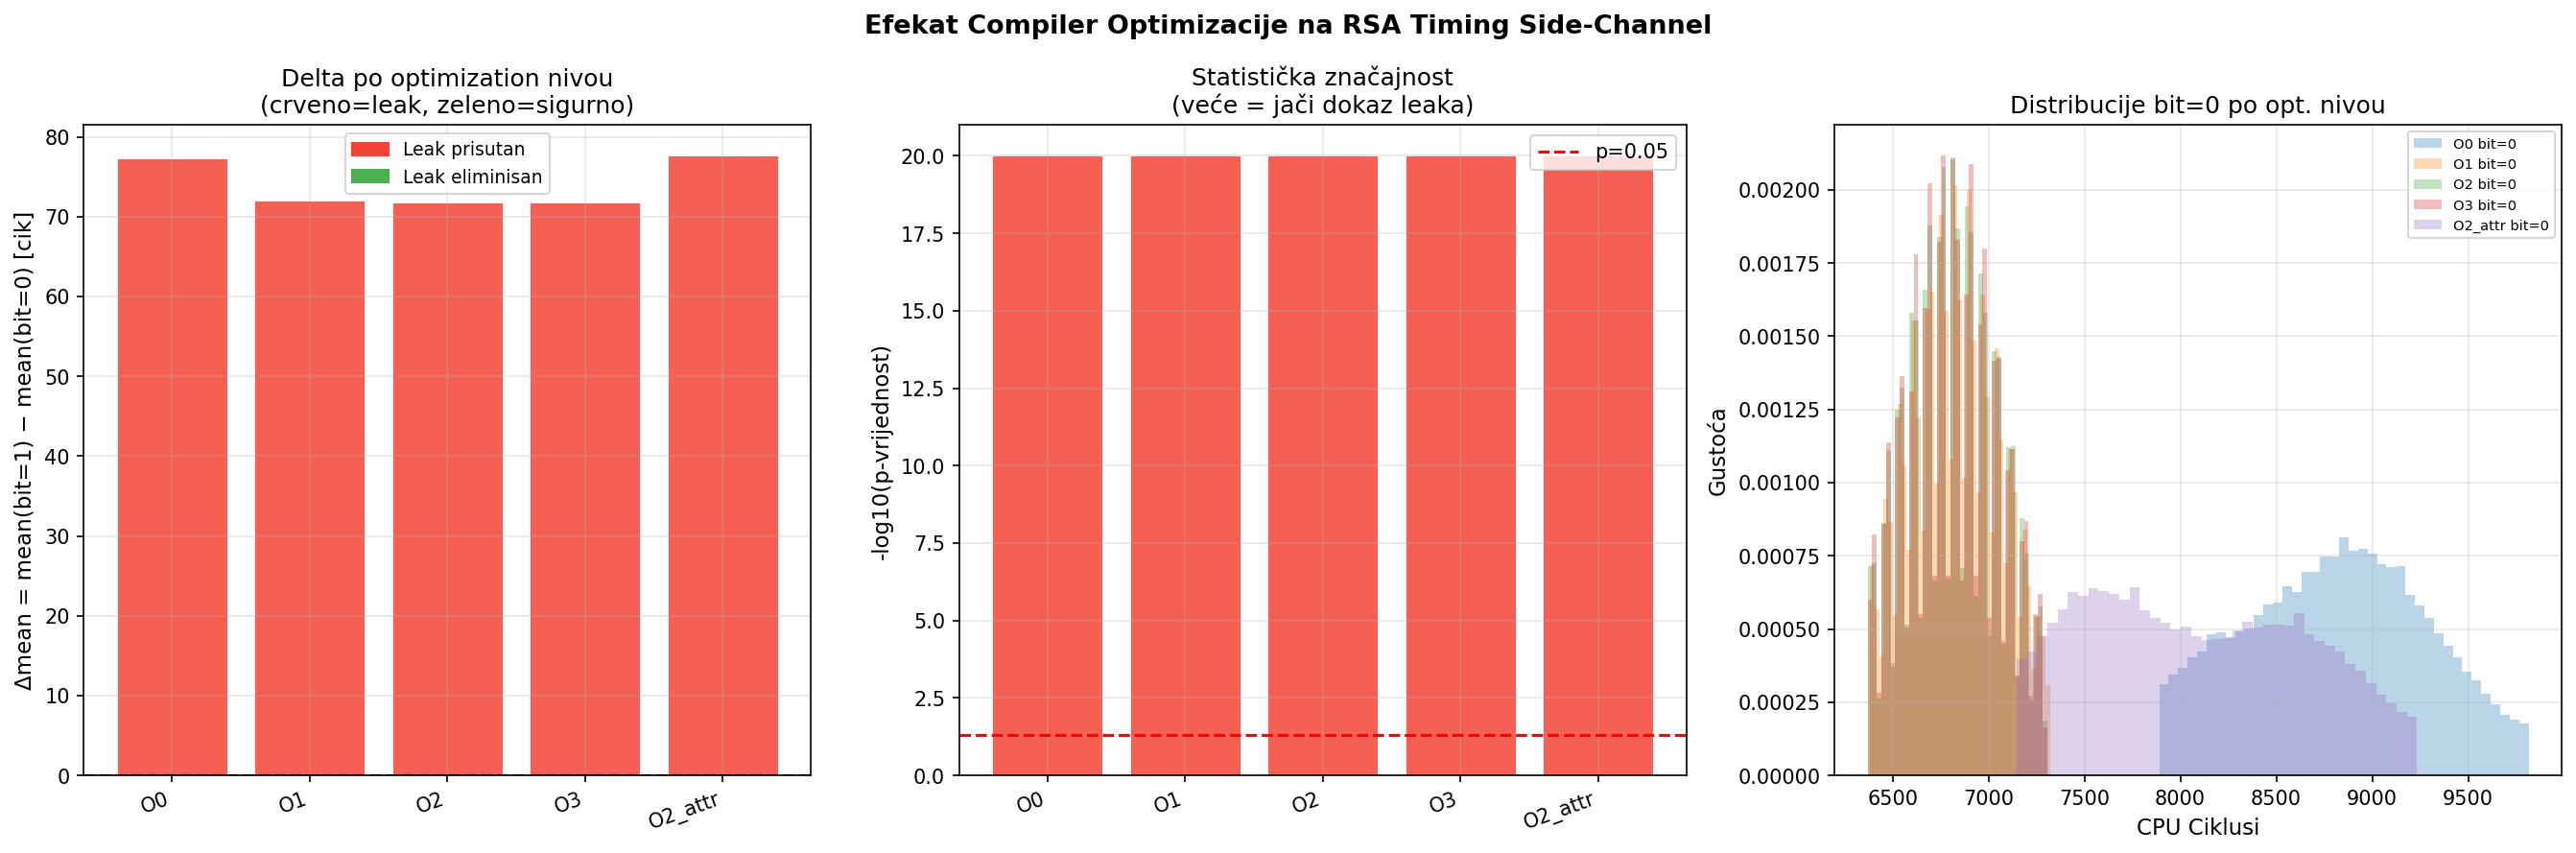
\includegraphics[width=\textwidth]{plot_compiler_effects.png}
\caption{Utjecaj kompajlerskih optimizacija: prosječna timing razlika $\Delta$ (u CPU ciklusima) i Cohen-ov $d$ za pet varijanti ranjive implementacije.}
\label{fig:compiler}
\end{figure}

Nijedan nivo optimizacije ne eliminiše vremensko curenje. Pregled asemblerskog koda za sve varijante (vidjeti Prilog \ref{app:asm_output}) potvrđuje da GCC ne transformiše grananje u \texttt{CMOV} instrukciju ni za jedan nivo optimizacije, a razlog je tehničke prirode: tijelo uslovnog bloka sadrži poziv funkcije (\texttt{mulmod}), a \texttt{CMOV} može zamijeniti samo jednostavne dodjele vrijednosti, ne pozive funkcija. Pri \texttt{-O0} i \texttt{O2+attr} kompajler generiše \texttt{je} (obrazac \texttt{shrx}/\texttt{and}/\texttt{test}/\texttt{je}), a pri \texttt{-O1}--\texttt{-O3} generiše \texttt{jae} (obrazac \texttt{bt}/\texttt{jae}); u oba slučaja radi se o uslovnom skoku koji mijenja putanju izvršavanja ovisno o vrijednosti tajnog bita.

Zanimljiv nalaz je da optimizacije \texttt{-O1} do \texttt{-O3} zapravo pojačavaju vremensku razliku Cohen-ov $d$ raste sa 0{,}136 (O0) na 0{,}267 (O1--O3), što je gotovo dvostruko povećanje. Fizičko objašnjenje: optimizirani kod drži varijable u registrima umjesto na steku i generiše kompaktniji pristup memoriji, što smanjuje ukupnu varijansu ($\sigma$). Budući da je signal ($\Delta \approx 72$ ciklusa) gotovo isti, manji šum daje veći odnos signala i šuma (SNR).

Varijanta ``O2+attr'' koristi \texttt{-O2} nivo za cijeli program, ali ciljanu funkciju označava atributom \texttt{optimize("O0")}. Ova varijanta ima nešto veći $\Delta$ (+77{,}62 naspram +71{,}73) ali manji Cohen-ov $d$ (0{,}120) jer neoptimizirana funkcija ima veću varijansu.

Ovaj eksperiment demonstrira da se programeri ne mogu osloniti na kompajlerske optimizacije kao sigurnosnu mjeru. Jedino eksplicitne vremenski konstantne implementacije, poput one opisane u sekciji \ref{sec:ct_impl}, garantuju odsustvo vremenskog curenja neovisno o kompajleru i nivou optimizacije.

% ---------------------------------------------------------------

\section{Eksperiment 6: Evaluacija RSA blindinga}

\subsection{Motivacija}

RSA blinding je kontramjera koju je OpenSSL implementirao nakon Brumley-Boneh napada \cite{brumley2003}. Principi standardnog RSA blindinga opisani su u sekciji \ref{sec:blinding_theory}. U ovom eksperimentu korištena je pojednostavljena varijanta blindinga:
\begin{align}
\text{blinded\_base} &= M \cdot r \bmod n \\
s' &= \text{blinded\_base}^d \bmod n
\end{align}

Unblinding u ovoj varijanti nije matematički egzaktan jer $(M \cdot r)^d \neq M^d \cdot r$, ali za analizu timing signala ispravnost krajnjeg rezultata nije relevantna. Ovaj pristup je validan jer mjerimo isključivo trajanje operacije eksponencijacije, ne njen izlaz, a nasumičan odabir baze vjerno replicira efekat blindinga na interne međuvrijednosti tokom eksponencijacije. Konkretno, promjenom baze mijenjaju se svi međurezultati tokom eksponencijacije, što je suštinski jednak efekt onome što standardni blinding postiže na vremensku distribuciju iako konačni rezultat nije matematički egzaktan dekript.

Eksperiment poredi blinded i unblinded varijantu sa oko 196\,000 uzoraka po varijanti.

\subsection{Rezultati}

\begin{table}[H]
\centering
\caption{Evaluacija RSA blindinga kao kontramjere}
\label{tab:blinding}
\begin{tabular}{lrrrrrl}
\toprule
\textbf{Varijanta} & \textbf{N} & \textbf{$\Delta$} & \textbf{t-stat} & \textbf{p-vrijednost} & \textbf{Cohen-ov $d$} & \textbf{Štiti?} \\
\midrule
Blinded     & 195\,999 & +65{,}30 & $-30{,}78$ & $9{,}3 \times 10^{-208}$ & 0{,}098 & Ne \\
Unblinded   & 196\,035 & +75{,}03 & $-39{,}15$ & $< 10^{-50}$              & 0{,}125 & Ne \\
\bottomrule
\end{tabular}
\end{table}

\begin{figure}[H]
\centering
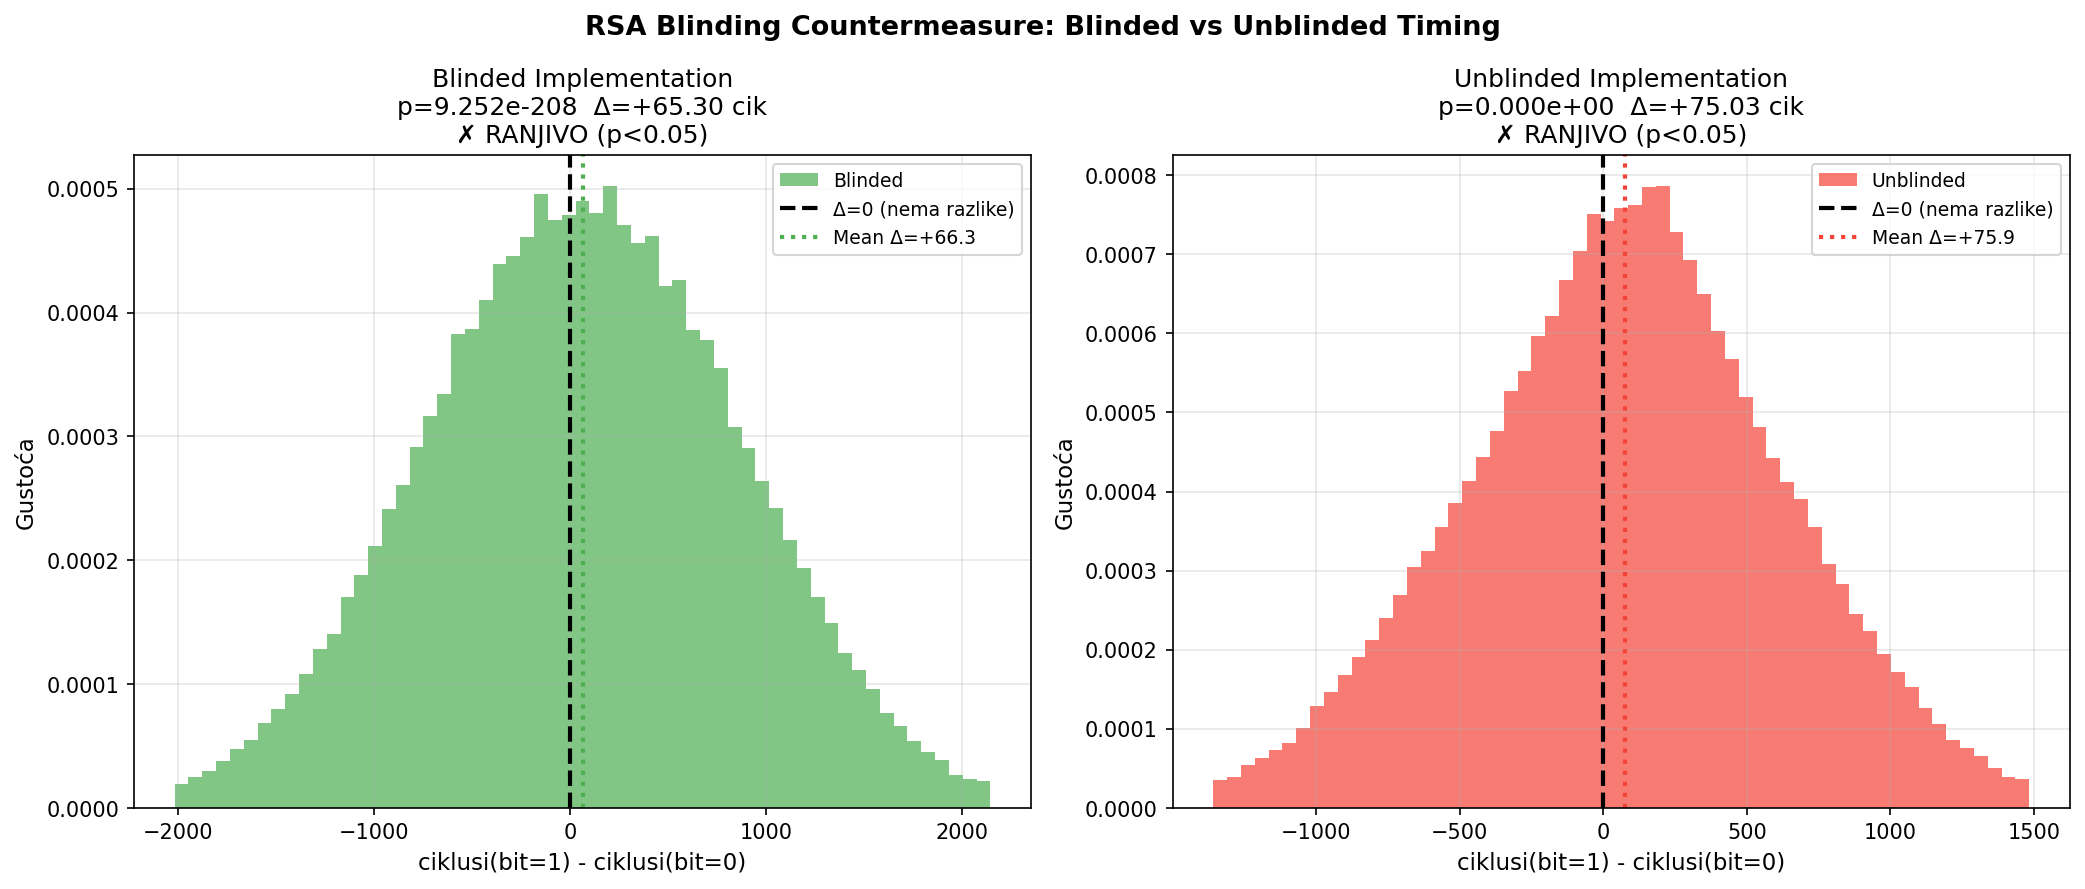
\includegraphics[width=\textwidth]{plot_blinding.png}
\caption{Evaluacija RSA blindinga kao kontramjere: distribucija parnih timing razlika za blinded (zelena) i unblinded (crvena) varijantu}
\label{fig:blinding}
\end{figure}

Blinding smanjuje timing razliku sa +75{,}03 na +65{,}30 ciklusa (redukcija od približno 13\%) i Cohen-ov $d$ sa 0{,}125 na 0{,}098. Međutim, signal i dalje ostaje statistički visoko značajan ($p = 9{,}3 \times 10^{-208}$), što znači da blinding ne eliminiše vremensko curenje.

Smanjenje signala od 13\% ima dva moguća objašnjenja. Prvo, instrukcija \texttt{MULQ} na testiranom procesoru možda ima male operand-zavisne timing varijacije koje blinding djelomično maskira promjenom ulaznih operanada. Drugo, blinded varijanta ima duže ukupno trajanje ($\approx 11\,740$ naspram $\approx 8\,770$ ciklusa za unblinded) jer koristi veće brojeve, što povećava apsolutnu varijansu i time razvodnjava relativnu veličinu signala. Razdvajanje ovih dviju hipoteza zahtijevalo bi izoliranu analizu latencije \texttt{MULQ}.

\subsection{Analiza: zašto blinding ne eliminiše leak}

Ovaj rezultat nije posljedica implementacijske greške, već fundamentalna posljedica arhitekture napada. U ovoj 64-bitnoj implementaciji, vremensko curenje dolazi od grananja u square-and-multiply algoritmu: za bit=1 izvršava se dodatni poziv \texttt{mulmod()} (grananje), dok se za bit=0 taj poziv preskače.

Blinding mijenja bazu (ulaz u množenje), ali ne mijenja eksponent $d$. Obrazac grananja \texttt{if ((exp >> i) \& 1)} ostaje identičan bez obzira na to koja je baza korištena. Dodatno, 64-bitna \texttt{MULQ} instrukcija na x86 izvršava množenje u konstantnom vremenu za sve operande, pa blinding ne može maskirati operand-zavisne varijacije jer ih na ovoj širini operanda praktično nema.

U realnom RSA s big-number aritmetikom (biblioteke poput GMP ili OpenSSL), situacija je suštinski drugačija. Višeprecizno množenje velikih brojeva (npr. 2048-bitnih) nije constant-time jer trajanje zavisi od efektivne veličine operanada i broja propagacija carry bita. U tom scenariju blinding randomizira međuvrijednosti i maskira operand-zavisni timing signal, čineći ga efikasnom kontramjerom \cite{brumley2003}.

Ovaj eksperiment demonstrira važnu razliku između dvije različite vrste vremenskog curenja:

\begin{description}
\item[Branch-zavisni leak] (korišten u ovim eksperimentima): Trajanje zavisi od kontrolnog toka, tj. od toga koji se put kroz kod izvršava. Blinding ne pomaže jer ne mijenja kontrolni tok.
\item[Operand-zavisni leak] (prisutan u realnom RSA s aritmetikom velikih brojeva): Trajanje zavisi od numeričke veličine operanada. Blinding pomaže jer nasumično bira operande čime onemogućuje napadaču da poveže trajanje s poznatim ulazom.
\end{description}

% ---------------------------------------------------------------

\section{Eksperiment 7: Flush+Reload cache napad}
\label{sec:fr_exp}

\subsection{Motivacija}

Eksperimenti 1--6 demonstriraju timing side-channel napade koji mjere ukupno trajanje kriptografske operacije. Međutim, postoji fundamentalno drugačija klasa napada koja umjesto ukupnog trajanja prati prisutnost specifičnih funkcija u CPU cache memoriji i njihovo vrijeme pristupa. Flush+Reload napad \cite{yarom2014} koristi fizički dijeljenu Last Level Cache (LLC) između procesa i može detektovati izvršavanje pojedinačnih funkcija iz dijeljene biblioteke bez mjerenja ukupnog trajanja.
\\

Ova klasa napada ima nekoliko praktičnih prednosti pred timing napadom. Napad funkcioniše čak i kada je žrtva na drugom CPU jezgru (bez dijeljenog L1/L2 cache-a), radi u prisustvu jačeg šuma (mrežna aktivnost, virtualizacija) jer signal ne zavisi od ukupnog trajanja operacije, i cilja specifičnu funkciju umjesto globalnog vremenskog signala.

Razlika od 341{,}5 ciklusa između cache hit-a i miss-a daleko je jača od vremenskog signala iz prethodnih eksperimenata (76 ciklusa), što čini klasifikaciju trivijalno lakom bez statističkog usrednjavanja.

\subsection{Princip Flush+Reload napada}

Princip Flush+Reload napada opisan je u sekciji \ref{sec:cache_attacks}: napadač u ciklusu izbacuje cache liniju ciljane funkcije (\texttt{clflush}), čeka da žrtva potencijalno izvrši operaciju, a potom mjeri reload latenciju. Kratka latencija ($\approx 340$ ciklusa) ukazuje na cache hit i zaključuje da je bit eksponenta jednak 1; duga latencija ($\approx 681$ ciklusa) ukazuje na cache miss i zaključuje da je bit jednak 0. Na x86 arhitekturi, svi procesi koji mapiraju isti \texttt{.so} fajl dobijaju iste fizičke okvire stranica, što je preduvjet za dijeljenu LLC cache memoriju.

\subsection{Implementacija}

Implementacijski detalji (dijeljeni RSA kod, pribavljanje adrese putem \texttt{dlsym()}, CPU pinning žrtve na zasebni fizički core i kalibracija praga) opisani su u sekciji~\ref{sec:fr_impl}. Žrtva između dekriptacija pauzira $50\,\mu\mathrm{s}$\footnote{Pri trajanju jedne dekriptacije od $\approx 4{,}2\,\mu\mathrm{s}$, aktivna frakcija iznosi $4{,}2/(4{,}2+50)\approx 7{,}7\,\%$ ukupnog vremena.}, što daje jasne granice između operacija i odgovara tipičnom primjeru kriptografskog servera s umjerenim opterećenjem.

\subsection{Rezultati}

\begin{table}[H]
\centering
\caption{Rezultati Flush+Reload napada na \texttt{rsa\_multiply\_step()}}
\label{tab:flush_reload}
\begin{tabular}{ll}
\toprule
\textbf{Metrika} & \textbf{Vrijednost} \\
\midrule
Broj observacija           & 100\,000 \\
Cache hitovi (bit=1)       & 45\,095 (45{,}1\%) \\
Cache miss-ovi (bit=0)     & 54\,905 (54{,}9\%) \\
Mean reload latencija (hit)  & 339{,}9 ciklusa \\
Mean reload latencija (miss) & 681{,}4 ciklusa \\
Razlika (miss $-$ hit)    & \textbf{341{,}5 ciklusa} \\
\bottomrule
\end{tabular}
\end{table}

\begin{figure}[H]
\centering
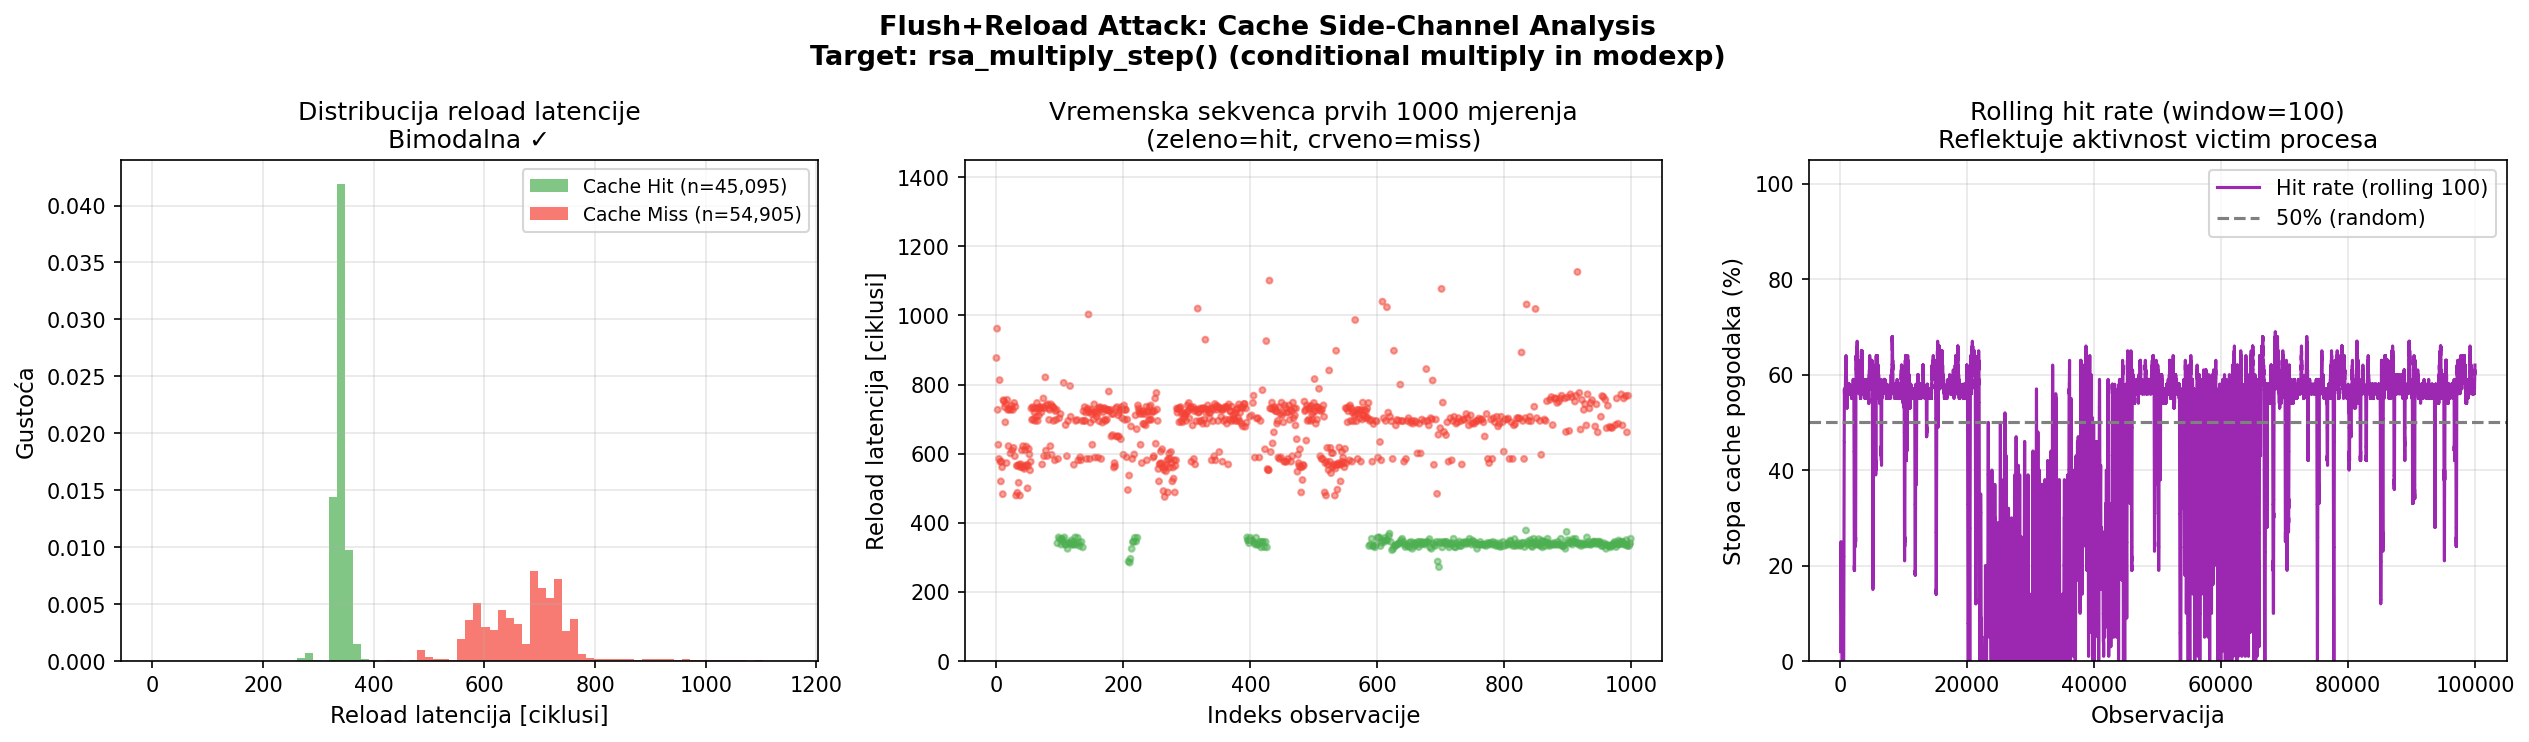
\includegraphics[width=\textwidth]{plot_flush_reload.png}
\caption{Histogram reload latencija: bimodalna distribucija, vremenska sekvenca mjerenja i rolling hit rate}
\label{fig:flush_reload}
\end{figure}

Slika \ref{fig:flush_reload} prikazuje bimodalnu distribuciju reload latencija sa dva jasno odvojena pika. Cache hit (žrtva je pozvala \texttt{rsa\_multiply\_step()}, što znači da je bit eksponenta jednak 1) daje prosječnu latenciju od 339{,}9 ciklusa, što odgovara latenciji pristupa LLC-u. Cache miss (funkcija nije bila pozvana) daje 681{,}4 ciklusa, što odgovara latenciji pristupa glavnoj memoriji (DRAM). Separacija od 341{,}5 ciklusa između cache hit-a i miss-a priblizno je 4{,}5 puta veća od timing signala iz prethodnih eksperimenata.

Udio cache hitova od 45{,}1\% je veći od naivne procjene zasnovane na aktivnoj frakciji i udjelu jediničnih bita ($7{,}7\% \times 72\% \approx 5{,}5\%$). Ova razlika objašnjava se perzistencijom podataka u LLC-u: kada žrtva pozove \texttt{rsa\_multiply\_step()}, odgovarajuća cache linija ostaje u LLC-u znatno duže od jednog intervala. Budući da se unutar jedne dekriptacije funkcija poziva za svaki od $\approx 34$ bita koji su jednaki 1, cache linija je prisutna u LLC-u tokom značajnog dijela aktivnog perioda žrtve, i napadač može detektovati hit čak i ako je konkretni poziv završio ranije.

\subsection{Poređenje s timing napadom}

Flush+Reload i timing napad ciljaju istu osnovnu ranjivost (uslovno grananje u square-and-multiply), ali koriste suštinski različite mehanizme detekcije:

\begin{table}[H]
\centering
\caption{Poređenje timing napada i Flush+Reload napada}
\label{tab:attack_comparison}
\begin{tabular}{lll}
\toprule
\textbf{Dimenzija} & \textbf{Timing napad (Eksperimenti 1--4)} & \textbf{Flush+Reload (Eksperiment 7)} \\
\midrule
Signal & $\approx 76$ ciklusa & $\approx 342$ ciklusa \\
Granularnost & Cijela operacija & Pojedinačna funkcija \\
Šum & Visok (OS, cache, TLB) & Nizak (bimodalna distribucija) \\
Mjerenja/bit & $K \geq 2000$ za 100\% & 1 mjerenje (threshold) \\
Dijeljeni resursi & Ništa & Dijeljeni LLC \\
Constant-time zaštita & Eliminiše napad & Eliminiše napad\footnotemark \\
\bottomrule
\end{tabular}
\end{table}

\footnotetext{Za Flush+Reload, zaštita je teoretski izvedena: constant-time implementacija izvršava obje operacije uvijek, pa bi ciljna funkcija bila prisutna u cache-u neovisno o vrijednosti bita. Ovo nije eksperimentalno verificirano u okviru ovog rada, i zahtijeva da obje putanje pristupaju istim cache linijama. Eksperimentalnu verifikaciju ove tvrdnje treba smatrati otvorenim pravcem za buduće istraživanje; u kontekstu ovog rada, zaštitu constant-time implementacije od Flush+Reload napada treba tretirati kao teorijsku pretpostavku, ne empirijsko tvrđenje.}

Najznačajnija razlika je u potrebnom broju mjerenja. Timing napad zahtijeva usrednjavanje $K = 2000$ mjerenja po bitu za postizanje 100\% tačnosti, dok Flush+Reload može klasificirati bit iz jednog jedinog mjerenja zahvaljujući daleko većem signalu (341 naspram 76 ciklusa). S druge strane, Flush+Reload zahtijeva da napadač i žrtva dijele istu fizičku memoriju (isti \texttt{.so} fajl), što ograničava primjenjivost na scenarije s dijeljenim bibliotekama.

Ova Flush+Reload implementacija je kontrolisani dokaz koncepta s namjerno izolovanom ciljnom funkcijom. U stvarnim kriptografskim bibliotekama, razlika između kvadriranja i množenja u funkcijama postojala je prirodno. 
Upravo takve prirodne separacije su motivisale Yarom i Falkner \cite{yarom2014} da demonstriraju ovaj napad i time potaknu prelazak na konstantne vremenske implementacije u modernim kriptografskim bibliotekama.

% ---------------------------------------------------------------
\section{Diskusija}

\subsection{Interpretacija Cohen-ovog d = 0{,}134}

Mali Cohen-ov $d$ ne umanjuje značaj nalaza. Ova vrijednost kvantificira fizičku veličinu efekta: signal od 76 ciklusa u šumu od $\sigma \approx 567$ ciklusa daje odnos signala i šuma (SNR) od 0{,}134 po pojedinačnom uzorku. Ovakav odnos je tipičan za timing napade na modernom procesoru, gdje su izvori šuma znatni (cache miss-ovi, pogrešna predviđanja grananja, preempcije operativnog sistema).

Ono što čini ovaj signal iskoristivim za napad je njegova konzistentnost i determinističnost. Signal se pojavljuje identično na medijani, P25 i P75 (Eksperiment 1), na svih 64 pozicija bita (Eksperiment 4), i pri različitim nivoima optimizacije (Eksperiment 5). Budući da je signal konzistentan a šum slučajan, usrednjavanje ga pouzdano "izvlači": $K = 2000$ uzoraka je dovoljno za 100\% tačnost klasifikacije (Eksperiment 2).


\subsection{Praktična cijena napada na realni RSA}

Eksperiment koristi 64-bitni privatni eksponent radi brzog izvođenja, ali mehanizam je identičan za realni RSA s 2048-bitnim ključem jer se svaki bit napada nezavisno istom tehnikom. Napad se konceptualno skalira linearno jer se informacije o bitovima privatnog eksponenta izdvajaju iterativno korištenjem iste metodologije mjerenja: za potpunu rekonstrukciju 2048-bitnog ključa potrebno je $2048 \times 5000 \times 2 \approx 20{,}5$ miliona mjerenja (5000 mjerenja po bitu, dva mjerenja po paru).

Pri prosječnom trajanju jedne 2048-bitne modularne eksponencijacije od $\approx 1$--$5$ ms (realistično za softversku aritmetiku velikih brojeva na standardnom savremenom procesoru), ukupno vrijeme napada iznosi od $\approx 5{,}7$ sati do $\approx 28{,}5$ sati. Sa CRT (\textit{Chinese Remainder Theorem} -- Kineski teorem o ostacima) optimizacijom koja ubrzava RSA dekriptovanje za faktor $\approx 4\times$, procjena se spušta na $\approx 1{,}4$--$7$ sati. Ovo ilustruje da timing napad nije isključivo teorijski, već je praktično izvodljiv u razumnom vremenskom okviru, pogotovo s obzirom na to da se napad može paralelizovati za pozicije bita.

U mrežnom scenariju svako mjerenje uvodi $\approx 0{,}1$--$1$ ms dodatne latencije, pa bi 20 miliona mjerenja trajalo od nekoliko sati do nekoliko dana, zavisno od mrežne udaljenosti i metode pojačavanja signala \cite{brumley2003}.

\subsection{Primjenjivost na moderne RSA biblioteke}

Napad demonstriran u ovom radu zasniva se na klasičnoj square-and-multiply implementaciji modularne eksponencijacije koja koristi eksplicitno grananje zavisno od vrijednosti bitova privatnog eksponenta. Savremene kriptografske biblioteke, poput \textit{OpenSSL}-a i \textit{libgcrypt}-a, uglavnom implementiraju različite zaštitne mehanizme kako bi se smanjilo curenje vremenskih informacija, čime se značajno otežava izvođenje klasičnih timing napada.

Ipak, zaštita od timing napada ne zavisi isključivo od algoritma, već i od načina implementacije aritmetike velikih brojeva. Implementacije koje ne koriste operacije konstantnog vremena nad operandima i dalje mogu otkrivati informacije kroz suptilne razlike u vremenu izvršavanja. Zbog toga manje poznate, prilagođene ili nestandardne kriptografske biblioteke mogu ostati ranjive čak i kada koriste moderne algoritamske optimizacije.



%Poglavlje 5
% poglavlje_5.tex — Zaključak

\chapter{Zaključak}
\label{ch:zakljucak}

\section{Pregled postignutih rezultata}

U ovom radu provedena je eksperimentalna analiza timing i cache timing side-channel napada nad RSA implementacijom zasnovanom na algoritmu kvadriraj-i-množi. Eksperimenti su provedeni na modernom hardveru (Intel i5-1335U, Raptor Lake) pod Ubuntu Linux operativnim sistemom, s preciznim mjerenjem CPU ciklusa. Ukupno je provedeno sedam eksperimenata koji pokrivaju detekciju vremenskog curenja, praktični napad rekonstrukcije ključa, sistematsku analizu svih bit-pozicija, evaluaciju kontramjera, te Flush+Reload cache napad.

Provedena analiza potvrdila je sve tri postavljene hipoteze: vremensko curenje u naivnoj kvadriraj-i-množi implementaciji je mjerljivo i iskoristivo, klasične kontramjere pokazuju ograničenja, a cache bazirani napadi nude znatno jači signal. Zajedno, ovi nalazi eksperimentalno demonstriraju na modernom hardveru ono što teorijska literatura predviđa, da kriptografska korektnost implementacije ne implicira njenu sigurnost.

Eksperimenti su potvrdili postojanje mjerljivog vremenskog curenja od $+75{,}90$ CPU ciklusa u naivnoj implementaciji (Cohen-ov $d = 0{,}134$, $p < 10^{-50}$), koje omogućava potpunu slijepu rekonstrukciju 64-bitnog privatnog ključa sa 100\% tačnošću, pri čemu napadački kod nikada nije imao pristup vrijednosti tajnog ključa. Analiza pozicija bita potvrdila je da curenje nije ograničeno na jednu poziciju, već je prisutno na svim 64 pozicijama. Implementacija s konstantnim vremenom potpuno eliminiše curenje ($d \approx 0$, $p = 0{,}84$), a tačnost napada pada na razinu slučajnog pogađanja ($\approx 50\%$).
\\

\section{Implikacije za praktičnu kriptografsku sigurnost}

\subsection{Neintuitivnost ranjivosti}
Naivna kvadriraj-i-množi implementacija matematički je potpuno ispravna i ranjivost ne leži u matematici nego u fizičkoj realizaciji, što ilustrira ključnu pouku: \textit{kriptografska sigurnost zahtijeva razmatranje izvedbe, a ne samo matematičke ispravnosti.} Ova neintuitivnost čini side-channel ranjivosti posebno opasnim: ne može ih otkriti ni formalna provjera ispravnosti ni standardno testiranje.

\subsection{Zavisnost od kompajlera nije sigurnost}
Eksperiment 5 potvrđuje da oslanjanje na kompajlerske optimizacije za sigurnosne mjere nije prihvatljiva opcija: nijedan testirani nivo nije generisao kod s konstantnim vremenom. Programer koji se osloni na kompajler ostaje nesvjesno izložen.

\subsection{Blinding ima ograničenja}
Eksperiment 6 pokazuje da blinding, iako efikasna kontramjera za operand-zavisne timing leake u realnom RSA \cite{brumley2003}, ne štiti od vremenskog curenja koje zavisi od grananja. Sigurna implementacija zahtijeva kombinaciju više tehnika: vremenski konstantne algoritme, blinding za maskiranje operand-zavisnih operacija u višepreciznoj aritmetici, te vremenski konstantne aritmetičke primitive.

\section{Ograničenja i mogući pravci daljeg istraživanja}

\subsection{Ograničenja}

\begin{enumerate}

\item \textbf{Veličina ključa (64 vs 2048+ bita).} Eksperiment koristi 64-bitni privatni eksponent i 61-bitni Mersenne modulus. Stvarni RSA koristi eksponente od 2048 do 4096 bita. Mehanizam je identičan za svaki bit, i napad se sa istim metodologijama skalira linearno s brojem bita, ali ukupno trajanje eksperimenta i broj potrebnih mjerenja proporcionalno rastu. Zaključci o detektabilnosti signala (Cohen-ov $d$, statistički testovi) direktno se prenose na veće ključeve jer su zasnovani na analizi po bitu.

\item \textbf{Jedna platforma (x86\_64, Intel Raptor Lake).} Svi eksperimenti provedeni su na jednoj mašini s jednim procesorom. Vrijednosti timing signala ($\approx 76$ ciklusa), razina šuma ($\sigma \approx 567$) i potreban broj mjerenja ($K = 2000$) specifični su za ovu arhitekturu, frekvenciju i njene karakteristike. ARM procesori, starije generacije Intela ili AMD platforme mogu imati drugačije karakteristike, što bi utjecalo na konkretne vrijednosti, ali ne i na korišten mehanizam curenja informacija.

\item \textbf{Lokalni model prijetnji (\textit{threat model}).} Napadač u ovom eksperimentu pokreće kod na istoj mašini kao i žrtva, bez mrežnog kašnjenja. Brumley i Boneh \cite{brumley2003} demonstrirali su da je napad izvodljiv i u mrežnom okruženju, ali uz daleko veći broj mjerenja i komplikovanije metode pojačavanja signala. Naš lokalni eksperimentalni postav idealizira uslove i daje značajno čišći signal od realnog mrežnog napada.

\item \textbf{Algoritam kvadriraj-i-množi ili moderni algoritmi.} Moderne kriptografske biblioteke (OpenSSL, libgcrypt) rijetko koriste naivni kvadriraj-i-množi s eksplicitnim grananjem. Ovaj rad demonstrira glavni princip, ali direktna primjena na moderne biblioteke zahtijevala bi analizu specifičnih implementacija. Ipak, razumijevanje naivne implementacije nužan je uslov za analizu komplikovanijih varijanti.

\end{enumerate}

\subsection{Pravci daljeg istraživanja}
Prirodni nastavak ovog rada mogao bi ići u dva smjera, i to prema realističnijem modelu prijetnji, ili prema složenijim kriptografskim primitivama:

\begin{itemize}
\item Analizu napada u mrežnom scenariju, replikacijom eksperimenta na mreži.
\item Evaluaciju Prime+Probe napada koji ne zahtijeva dijeljenu memoriju i radi između virtualnih mašina.
\item Analizu timing napada na eliptičnu kriptografiju (ECDSA, ECDH), gdje su side-channel ranjivosti kompleksnije ali prisutne.
\item Analizu timing napada nad postkvantnim algoritmima.
\end{itemize}

\noindent Rezultati potvrđuju da timing i cache side-channel napadi na RSA imaju praktičnu primjenjivost na modernom hardveru, i dok kriptografski algoritmi postaju sve robusniji, sigurnost implementacije ostaje otvoren problem koji zahtijeva jednaku pažnju kao i matematički temelji na kojima počivaju.



%%%%%%%%%%%%%%%%%%%%% PRILOZI %%%%%%%%%%%%%%%%%%%%%%%%%%%%%%%%%%%%
\begin{appendices}
%Priloge je najbolje raditi u odvojenim fajlovima
%Prilog 1
\chapter{Konfiguracija hardverskog okruženja}
\label{app:hw_config}

Ovaj prilog dokumentuje detaljne korake konfiguracije hardverskog okruženja primijenjene prije pokretanja eksperimenata. Ove mjere osiguravaju reproducibilnost i minimizaciju sistematskog šuma.

\section{Isključivanje Turbo Boost-a}

Intel Turbo Boost dinamički podiže frekvenciju procesora (do 4{,}6 GHz na i5-1335U) ovisno o termičkom stanju. Budući da TSC raste po konstantnoj stopi (nominalnoj frekvenciji), aktivan Turbo znači da isti broj TSC ciklusa odgovara različitoj količini stvarnog rada. Isključivanje:

\begin{lstlisting}[language=bash, caption={Isključivanje Intel Turbo Boost-a}]
echo 1 | sudo tee /sys/devices/system/cpu/intel_pstate/no_turbo
\end{lstlisting}

\section{Performance CPU governor}

Podrazumijevani \texttt{powersave} governor (korišten s \texttt{intel\_pstate} driverom na ovoj platformi) dinamički prilagođava frekvenciju, što bi uzrokovalo da početne iteracije rade na nižoj frekvenciji:

\begin{lstlisting}[language=bash, caption={Postavljanje performance governor-a}]
sudo cpupower frequency-set -g performance
\end{lstlisting}

\section{CPU pinning}

Intel i5-1335U ima P-core (Raptor Cove, out-of-order, 3{,}4 GHz baza) i E-core (Gracemont, out-of-order, 2{,}5 GHz) jezgre s različitim latencijama. Bez eksplicitnog odabira, Linux scheduler može migrirati procese između jezgri:

\begin{lstlisting}[language=bash, caption={Pokretanje eksperimenta s fiksiranjem na P-core 0}]
taskset -c 0 ./experiment
\end{lstlisting}

Dodatno, eksperimentalni program programski poziva \texttt{sched\_setaffinity()} kao drugi nivo osiguranja.

\section{Zagrijavanje cache-a}

Prvih 10\,000 iteracija eksperimenta je faza zagrijavanja čija se mjerenja odbacuju. Svrha:
\begin{itemize}
\item Populacija L1/L2 cache memorije relevantnim kodom i podacima
\item Stabilizacija branch prediktora
\item Termalna stabilizacija procesora (eliminacija thermal throttling-a)
\end{itemize}

\section{Verifikacija TSC frekvencije}

Program mjeri TSC frekvenciju poređenjem TSC-a i \texttt{CLOCK\_MONOTONIC} sata tokom 100 ms intervala. Izmjereno: $\approx 2{,}101$ GHz (odgovara nominalnoj frekvenciji).

\section{Provjera assembly izlaza}

Za verifikaciju da kompajler ne generiše \texttt{CMOV} instrukcije:

\begin{lstlisting}[language=bash, caption={Provjera assembly koda za branch instrukcije}]
make check-asm-all
# Ocekivani izlaz: jne/je (branch), nikad cmov
\end{lstlisting}

\section{Assembly izlaz: implementacija sa grananjem i bez grananja}
\label{app:asm_output}

Za verifikaciju da je timing ranjivost prisutna na nivou mašinskog koda, ispod su prikazani ključni dijelovi assembly izlaza dobijenog naredbom \texttt{objdump~-d}. Korišten je GCC~13.3 na Ubuntu~24.04.

\subsection{Ranjiva implementacija (eksplicitni branch)}

Isječak koda \ref{lst:asm_vuln} prikazuje kritični uslovni skok u funkciji \texttt{mod\_exp\_vulnerable}. Instrukcija \texttt{je} (jump if equal / jump if zero) preskače blok množenja kada je bit eksponenta 0, čime nastaje mjerljiva timing razlika.

\begin{lstlisting}[caption={Ključni uslovni skok (\textit{branch}) u \texttt{mod\_exp\_vulnerable} -- stvarni \texttt{objdump} izlaz (GCC 13.3, \texttt{-O0}, Intel sintaksa)}, label=lst:asm_vuln, basicstyle=\ttfamily\small, numbers=none]
; Testiranje bita eksponenta: if ((exp >> i) & 1)
208b:    mov    eax,DWORD PTR [rbp-0xc]      ; ucitaj i (loop counter)
208e:    mov    rdx,QWORD PTR [rbp-0x20]     ; ucitaj exp
2092:    shrx   rax,rdx,rax                  ; rax = exp >> i
2097:    and    eax,0x1                      ; rax = (exp >> i) & 1
209a:    test   rax,rax
209d:    je     20ba <mod_exp_vulnerable+0x89>  ; USLOVNI SKOK: preskok za bit=0
; --- blok mnozenja: izvrsava se SAMO za bit=1 ---
209f:    mov    rdx,QWORD PTR [rbp-0x28]     ; ucitaj mod
20a3:    mov    rcx,QWORD PTR [rbp-0x18]     ; ucitaj base
20a7:    mov    rax,QWORD PTR [rbp-0x8]      ; ucitaj result
20ab:    mov    rsi,rcx
20ae:    mov    rdi,rax
20b1:    call   1f8d <mulmod>                ; poziv mulmod(result, base, mod)
20b6:    mov    QWORD PTR [rbp-0x8],rax      ; pohrani result
; --- obje grane spajaju se ovdje ---
20ba:    sub    DWORD PTR [rbp-0xc],0x1      ; i--
\end{lstlisting}

\subsection{Konstantna vremenska implementacija (branchless)}

Za usporedbu, isječak koda \ref{lst:asm_ct} prikazuje \texttt{ct\_select()} selekciju u konstantnoj vremenskoj implementaciji. Umjesto uslovnog skoka, koriste se isključivo aritmetičke i logičke instrukcije koje se izvršavaju u konstantnom vremenu bez obzira na vrijednost bita.

\begin{lstlisting}[caption={Selekcija bez grananja (\textit{branchless}) u \texttt{mod\_exp\_constant\_time}}, label=lst:asm_ct, basicstyle=\ttfamily\small, numbers=none]
  ; ct_select(bit, mul_result, result) -- bez grananja
  movq   %rdi, %rax          ; load bit
  andl   $0x1, %eax          ; bit & 1
  negq   %rax                ; mask = -(bit & 1)
  movq   %rax, %rcx          ; rcx = mask
  andq   %rsi, %rcx          ; mul_result & mask
  notq   %rax                ; ~mask
  andq   %rdx, %rax          ; result & ~mask
  orq    %rcx, %rax          ; combine: finalni rezultat
\end{lstlisting}

\noindent CPU izvršava identičnu sekvencu instrukcija bez obzira na vrijednost bita i nema uslovnih skokova, nema branch predikcije, nema timing razlike.

\end{appendices}

%%%%%%%%%%%%%%%%%%%%%%%%%%%%%%%%%%%%%%%%%%%%%%%%%%%%%%%%%%%%%%%%%%%
\backmatter

%%%%%%%%%%%%%%%%%%%%%%% LITERATURA %%%%%%%%%%%%%%%%%%%%%%%%%%%%%%%%%
\addcontentsline{toc}{chapter}{Literatura}
\bibliographystyle{IEEEtranETF} 
\bibliography{literatura}

% Indeks pojmova izostavljen -- nema \index{} unosa u tekstu rada.
% \addcontentsline{toc}{chapter}{Indeks pojmova}
% \printindex


\end{document}
